%input macros (i.e. write your own macros file called MacroFile1.tex)
\newcommand{\PdfPsText}[2]{
  \ifpdf
     #1
  \else
     #2
  \fi
}

\newcommand{\IncludeGraphicsH}[3]{
  \PdfPsText{\includegraphics[height=#2]{#1}}{\includegraphics[bb = #3, height=#2]{#1}}
}

\newcommand{\IncludeGraphicsW}[3]{
  \PdfPsText{\includegraphics[width=#2]{#1}}{\includegraphics[bb = #3, width=#2]{#1}}
}

\newcommand{\InsertFig}[3]{
  \begin{figure}[!htbp]
    \begin{center}
      \leavevmode
      #1
      \caption{#2}
      \label{#3}
    \end{center}
  \end{figure}
}


 
 






\newcommand{\sltz}{SL_2(\mathbb{Z})}
\newcommand{\sltznz}[1][N]{SL_2(\mathbb{Z}/#1\mathbb{Z})}
\newcommand{\psltznz}[1][N]{PSL_2(\mathbb{Z}/#1\mathbb{Z})}
\newcommand{\psltz}{PSL_2(\mathbb{Z})}
\newcommand{\sltr}{SL_2(\mathbb{R})}

\newcommand{\pmi}{\{\pm I_2 \}}
\newcommand{\abcd}{\left(\begin{array}{ c c } a & b \\ c & d \end{array} \right)}
\newcommand{\sm}{\left(\begin{array}{ c c } 0 & -1 \\ 1 & 0 \end{array} \right)}
\newcommand{\tm}[1][1]{\left(\begin{array}{ c c } 1 & #1 \\ 0 & 1 \end{array} \right)}
\newcommand{\um}[1][1]{\left(\begin{array}{ c c } 1 & 0 \\ #1 & 1 \end{array} \right)}
\newcommand{\mobh}{\text{M{\"o}b}(\mathcal{H})}

\newcommand{\znz}[1][N]{\mathbb{Z}/#1\mathbb{Z}}


\newcommand{\myqed}{$\square$}



\makeatletter
\newsavebox\myboxA
\newsavebox\myboxB
\newlength\mylenA

\newcommand*\xoverline[2][0.75]{%
    \sbox{\myboxA}{$\m@th#2$}%
    \setbox\myboxB\null% Phantom box
    \ht\myboxB=\ht\myboxA%
    \dp\myboxB=\dp\myboxA%
    \wd\myboxB=#1\wd\myboxA% Scale phantom
    \sbox\myboxB{$\m@th\overline{\copy\myboxB}$}%  Overlined phantom
    \setlength\mylenA{\the\wd\myboxA}%   calc width diff
    \addtolength\mylenA{-\the\wd\myboxB}%
    \ifdim\wd\myboxB<\wd\myboxA%
       \rlap{\hskip 0.5\mylenA\usebox\myboxB}{\usebox\myboxA}%
    \else
        \hskip -0.5\mylenA\rlap{\usebox\myboxA}{\hskip 0.5\mylenA\usebox\myboxB}%
    \fi}
\makeatother
%%% Local Variables: 
%%% mode: latex
%%% TeX-master: "~/Documents/LaTeX/CUEDThesisPSnPDF/thesis"
%%% End: 


 \documentclass[oneside,10pt]{Classes/CUEDthesisPSnPDF}


\ifpdf
    \pdfinfo { /Title  (Marco Forte Math research project )
               /Creator (TeX)
               /Producer (pdfTeX)
               /Author (Marco Forte fortemarco.irl@gmail.com)
               /CreationDate (D:201604121000)  %format D:YYYYMMDDhhmmss
               /ModDate (D:20030815213532)
               /Subject (Writing a PhD thesis in LaTeX)
               /Keywords (PhD, Thesis)}
    \pdfcatalog { /PageMode (/UseOutlines)
                  /OpenAction (fitbh)  }
\fi

\title{Congruence and non-congruence subgroups of $SL_2(\mathbb{Z})$}

\ifpdf
  \author{\href{mailto:fortemarco.irl@gmail.com}{Marco Forte}}
  \collegeordept{\href{http://www.ucd.ie/mathstat/}{School of Mathematics and Statistics}}
  \university{\href{http://www.ucd.ie}{University College Dublin}}
% insert below the file name that contains the crest in-place of 'UnivShield'
\crest{
\includegraphics[width=30mm]{UnivShield}}
\else
  \author{Marco Forte}
  \collegeordept{School of Mathematics and Statistics}
  \university{University College Dublin}
% insert below the file name that contains the crest in-place of 'UnivShield'
  \crest{
\includegraphics[bb = 0 0 292 336, width=30mm]{UnivShield}}
\fi
%
% insert below the file name that contains the crest in-place of 'UnivShield'
% \crest{\IncludeGraphicsW{UnivShield}{40mm}{14 14 73 81}}
%
\renewcommand{\submittedtext}{Undergraduate research project \\
Supervisor: Dr. Kevin Hutchinson}
\degree{}
\degreedate{May 2016}

% turn of those nasty overfull and underfull hboxes
\hbadness=10000
\hfuzz=50pt

% Put all the style files you want in the directory StyleFiles and usepackage like this:
\usepackage{StyleFiles/watermark}
\usepackage[utf8]{inputenc}
\usepackage{enumerate}
\usepackage{amssymb}
\usepackage{amsmath}
\usepackage{ellipsis}
\usepackage{amsfonts}
\usepackage{todonotes}
\usepackage{amsthm}
\usepackage{caption}
\usepackage{subcaption}
\usepackage{xr}

% Comment out the next line to get single spacing
\onehalfspacing

\begin{document}

%\language{english}

% A page with the abstract on including title and author etc may be
% required to be handed in separately. If this is not so, then comment
% the below 3 lines (between '\begin{abstractseparte}' and 
% 'end{abstractseparate}'), normally like a declaration ... needs some more
% work, mind as environment abstracts creates a new page!
%\begin{abstractseparate}
%  
% Thesis Abstract -----------------------------------------------------


%\begin{abstractslong}    %uncommenting this line, gives a different abstract heading
\begin{abstracts}        %this creates the heading for the abstract page

The theory of linear groups goes back to the foundation of group theory. Évariste Galois constructed the groups $PSL(2,p)$ were constructed by Évariste Galois in the 1830s, he also constructed the general linear group over a prime field, $GL(n, p)$, in studying the Galois group of the general equation of degree $p^n$. The existence of non-congruence subgroups was known to Felix Klein who made extensive contribution in the related field of modular forms. This project give's an undergraduate accessible exposition of the theory of congruence and non-congruence subgroups. A goal of the project was to give a more detailed report sized overview of the theory. \\
\\

\textbf{Acknowledgements}: I would like to thank Dr. Kevin Hutchinson for his excellent mentoring and support over the months of the module. I believe his guidance has enabled to do far more than I thought I was capable of and helped me become a much better mathematics student. I would also like to mention Dr. Keith Conrad for his superb collection of expository papers, especially the one on $SL_2(\mathbb{Z})$ \citep{conrad} which served as the initial motivation for beginning this project. \\
I would also like to thank University College Dublin and University of California: Santa Cruz for high quality mathematics education I have been given.
 

\end{abstracts}
%\end{abstractlongs}


% ----------------------------------------------------------------------


%%% Local Variables: 
%%% mode: latex
%%% TeX-master: "../thesis"
%%% End: 

%\end{abstractseparate}




% Using the watermark package which is in StyleFiles/
% and to remove DRAFT COPY ONLY appearing on the top of all pages comment out below line
%\watermark{DRAFT COPY ONLY}


\maketitle

%set the number of sectioning levels that get number and appear in the contents
\setcounter{secnumdepth}{3}
\setcounter{tocdepth}{3}

\frontmatter % book mode only
\pagenumbering{roman}
%% Thesis Acknowledgements ------------------------------------------------


%\begin{acknowledgementslong} %uncommenting this line, gives a different acknowledgements heading
\begin{acknowledgements}      %this creates the heading for the acknowlegments


And I would like to acknowledge ...


\end{acknowledgements}
%\end{acknowledgmentslong}

% ------------------------------------------------------------------------

%%% Local Variables: 
%%% mode: latex
%%% TeX-master: "../thesis"
%%% End: 


% Thesis Abstract -----------------------------------------------------


%\begin{abstractslong}    %uncommenting this line, gives a different abstract heading
\begin{abstracts}        %this creates the heading for the abstract page

The theory of linear groups goes back to the foundation of group theory. Évariste Galois constructed the groups $PSL(2,p)$ were constructed by Évariste Galois in the 1830s, he also constructed the general linear group over a prime field, $GL(n, p)$, in studying the Galois group of the general equation of degree $p^n$. The existence of non-congruence subgroups was known to Felix Klein who made extensive contribution in the related field of modular forms. This project give's an undergraduate accessible exposition of the theory of congruence and non-congruence subgroups. A goal of the project was to give a more detailed report sized overview of the theory. \\
\\

\textbf{Acknowledgements}: I would like to thank Dr. Kevin Hutchinson for his excellent mentoring and support over the months of the module. I believe his guidance has enabled to do far more than I thought I was capable of and helped me become a much better mathematics student. I would also like to mention Dr. Keith Conrad for his superb collection of expository papers, especially the one on $SL_2(\mathbb{Z})$ \citep{conrad} which served as the initial motivation for beginning this project. \\
I would also like to thank University College Dublin and University of California: Santa Cruz for high quality mathematics education I have been given.
 

\end{abstracts}
%\end{abstractlongs}


% ----------------------------------------------------------------------


%%% Local Variables: 
%%% mode: latex
%%% TeX-master: "../thesis"
%%% End: 


\tableofcontents
%\listoffigures
%\printnomenclature  %% Print the nomenclature
%\addcontentsline{toc}{chapter}{Nomenclature}

\mainmatter % book mode only

\newtheorem{theorem}{Theorem}[section]
\newtheorem{lemma}[theorem]{Lemma}
\newtheorem{proposition}[theorem]{Proposition}
\newtheorem{corollary}[theorem]{Corollary}
\theoremstyle{definition}
\newtheorem{example}[theorem]{Example}
\theoremstyle{definition}
\newtheorem{remark}[theorem]{Remark}
\theoremstyle{definition}
\newtheorem{definition}[theorem]{Definition}


%%% Thesis Introduction --------------------------------------------------
\chapter{Preliminary group theory}
\ifpdf
    \graphicspath{{Introduction/IntroductionFigs/PNG/}{Introduction/IntroductionFigs/PDF/}{Introduction/IntroductionFigs/}}
\else
    \graphicspath{{Introduction/IntroductionFigs/EPS/}{Introduction/IntroductionFigs/}}
\fi



The level of this project is aimed at final year undergraduate mathematics students. Knowledge of basic group theory, number theory, complex numbers is assumed. We us some more specialised theory that readers may be unaware of or might need a quick refresh. So this prelimanary chapter contains definitions and results of this kind. \\

\section{Group Actions}
\begin{definition}\label{def:groupAction}
A group action of a group $G$ on a set $A$ is the map from $G \times A$ to $A$ (written as $ g \cdot a$, for for all $g \in G$ and $a \in A$) satisfying the following properties:
\begin{enumerate}
\item $g_1\cdot(g_2 \cdot a) = (g_1g_2) \cdot s$  for all  $g_1, g_2 \in G, a \in A$, 
\item $1 \cdot a = a$, for all $a \in A$
\end{enumerate}
The set $A$ is called a $G$-set.
\end{definition}
We often refer to this as $G$ is a group acting on a set $A$. The expression $g \cdot a $ will usually be written simply as $ga$ or $g(a)$.

\begin{definition}
Let $A$ be a $G$-set. The \textit{stabilizer} of $a \in A$ is the set, 
$$ G_a = \{g \in G \, \vert \, g \cdot a = a \}$$
\end{definition}

\begin{proposition}
Let $A$ be a $G$-set. The relation $~$ on $A$ defined by $a ~ b$ if and only if $b = g\cdot a $ for some $g \in G$ is an equivalence relation on $A$.
\end{proposition}

\begin{definition}
The equivalence class of $a \in A$ is called the orbit of $a$.
\end{definition}
We using equivalence and orbit we often refer to the group explicitly, we say the points $a,b$ are $G$-equivalent and $a,b$ in the same $G$-orbit. \\
\\

\section{Isomorphism Theorems}
\begin{theorem}{First Isomorphism Theorem}
Let $\theta \, : G \rightarrow H$ be a group homomorphism. Then
$$ G/ker\theta \cong Im \theta$$
\end{theorem}

\begin{theorem}{Third Isomorphism / Factor of a factor Theorem}
Let $M,N$ be normal subgroups of the group $G$ with $M$ contained in $N$. Then,
\begin{enumerate}
\item $N/M$ is a normal subgroup of $G/M$ and
\item $(G/M)/(N/M) \cong G/N$
\end{enumerate}
\end{theorem}

\begin{theorem}{Fourth Isomorphism / Correspondence theorem}
Let $N$ be a normal subgroup of $G$, let $H$ be a subgroup of $G$. The mapping $H \mapsto H/N$ defines a bijection between the set of subgroups of $G$ containing $N$ and the set of subgroups of $G/N$. Furthermore this correspondence preserves normality.
\end{theorem}

\section{Jordan-Holder Theorem}
\begin{definition}{Internal / external direct product}

A group $G$ is an (internal) direct product $H_1 \times \cdots \times H_n$ of subgroups $H_1, \ldots, H_n$ if 
\begin{enumerate}
\item $H_i \trianglelefteq G$ for $i = 1, \ldots , n$ and 
\item every element $g \in G$ can be uniquely written in the form 
$$g = h_1 \cdots h_n$$
with $h_i \in H_i$.
\end{enumerate}

The external direct product is defined as the n-tuples $(h_1, \ldots, h_n)$ with $h_i \in H_i$, with multiplication
$$ (g_1, \ldots, g_n)(h_1, \ldots h_n ) = (g_1 h_1,\ldots,g_n h_n)$$
\end{definition}

\begin{definition}
A \textbf{normal series} for a group $G$ is a chain
$$ G = G_0 \geq G_1 \geq \cdots \geq G_r = \{1\}$$
of normal subgroups of $G$.
\end{definition}

\begin{definition}
A \textbf{subnormal series} for a group $G$ is a chain
$$ G = G_0 \geq G_1 \geq \cdots \geq G_r = \{1\}$$
of subgroups of $G$ with $G_i \trianglelefteq G_{i+1}$.
\end{definition}

\begin{definition}
Let 
$$ G = G_0 \geq G_1 \geq \cdots \geq G_r = \{1\}$$
and
$$ H = H_0 \geq H_1 \geq \cdots \geq H_s = \{1\}$$
be two normal (or subnormal series) for $G$.
\begin{enumerate}[(a)]
\item Then the second series is a \textbf{refinement} of the first if each group which appears in the first series also appears in the second.
\item The two series are \textbf{isomorphic} if there exists a bijection from 
$$\{G_0/G_1, G_1/G_2, \ldots , G_{r-1}/G_r \} \rightarrow \{ H_0/H_1, \ldots , H_{s-1}/H_s\}$$
such that the quotient groups that correspond under the bijection are isomorphic. 
\end{enumerate}
\end{definition}

\begin{definition}
A normal series for a group $G$ with no repeated terms which cannot be refined except by repeating terms is called a \textbf{chief} series for $G$.
\end{definition}


\begin{definition}
A subnormal series for a group $G$ with no repeated terms which cannot be refined except by repeating terms is called a \textbf{composition} series for $G$.
\end{definition}

\begin{theorem}{(Jordan-Holder Theorem).} If a group has a chief (or composition) series then any two chief (or composition) series are isomorphic.
\end{theorem}

\section{Free groups}
The following exposition on free groups is taken directly from section 6.3 of the book Abstract Algebra \citep{dummit}. Only the relevant informal discussion is included here, there is much more detailed discussion available in the book. \\

The basic idea of a free group $F(S)$ generated by a set $S$ is that there are no relations satisfied by any of the elements in $S$ ( $S$ is "free" of relations). For example, if $S$ is the
set $\{a, b\}$ then the elements of the free group on the two generators $a$ and $b$ are of the
form $a, aa, ab, abab, bab,$ etc., called words in $a$ and $b$, together with the inverses of
these elements, and all these elements are considered distinct. If we group like terms
together, then we obtain elements of the familiar form $a$, $b^-3$, $aba^-1b^2$ etc. Such
elements are multiplied by concatenating their words (for example, the product of $aba$
and $b^-1a^3b$ would simply be $abab^-1a^3b$). It is natural at the outset (even before we
know $S$ is contained in some group) to simply define $F(S)$ to be the set of all words in $S$,
where two such expressions are multiplied in $F(S)$ by concatenating them. \\
\\
One important property reflecting the fact that there are no relations that must be
satisfied by the generators in $S$ is that any map from the set $S$ to a group $G$ can be
uniquely extended to a homomorphism from the group $F(S)$ to $G$ (basically since we
have specified where the generators must go and the images of all the other elements
are uniquely determined by the homomorphism property - the fact that there are
no relations to worry about means that we can specify the images of the generators
arbitrarily). This is frequently referred to as the universal property of the free group
and in fact characterizes the group $F(S)$.
\\

\begin{definition}
The group $F(S)$ is called the free group on the set $S$. A group $F$ is a free
group if there is some set $S$ such that $F = F(S)$ - in this case we call $S$ a set of free
generators (or a free basis) of $F$. The cardinality of $S$ is called the rank of the free
group.
\end{definition}

\begin{definition}
Let $S$ be a subset of a group $G$ such that $G = \langle S \rangle$.\\
A presentation for $G$ is a pair $(S, R)$, where $R$ is a set of words in $F(S)$ such that
the normal closure of $\langle R \rangle$ in $F(S)$ (the smallest normal subgroup containing
$\langle R \rangle$ ) equals the kernel of the homomorphism $\pi : F (S) \rightarrow G$ (where $\pi$ extends the identity map from $S$ to $S$). The elements of $S$ are called generators and those
of $R$ are called relations of $G$.\\
We say $G$ is \textbf{finitely generated} if there is a presentation $(S,R)$ such that $S$ is a finite set, and we say $G$ is finitely presented if there is a presentation $(S, R)$ with
both $S$ and $R$ finite sets.
\end{definition}

The following comes from Chapter 11 of the book An introduction to the theory of groups \citep{rotmanFree}.
\begin{definition}
The free product $ G \star H$ of groups $G$ and $H$ is the set of elements of the form
$$ g_1h_1 g_2h_2 \cdots g_r h_r, $$
where $g_i$ in $G$ and $h_i$ in $H$, with $g_1$ and $h_r$ possibly equal to $e$, the identity element of $G$ and $H$.
\end{definition}

\begin{definition}
Let $S$ be a subset of the group $G$.
A \textbf{word} on $S$ is a sequence $w = (s_1,s_2,\ldots)$, where $s_i \in S \cup S^{-1} \cup \{1\}$ for all $i$, such that all $i =1$ from some point on. The \textbf{length} of $w = s_1^{a_1}\cdots s_n{a_n}$ is defined to be $n$.\\
Since words contain only a finite number of letter before they become constant, we use the more suggestive notation for non-identity words,
$$ w = s_1^{a_1}s_2^{a_2}\cdots s_n{a_n}$$
where $s_i \in S$, $a_i = \pm 1$ or $0$, and $a_n = \pm 1$.
\end{definition}
\begin{definition}
If $w =  s_1^{a_1}\cdots s_n{a_n}$ is a word, then it's \textbf{inverse} is the word $w^{-1} =  s_1^{-a_1}\cdots s_n{-a_n}$.
\end{definition}
\begin{definition}
A word $w$ on $S$ is \textbf{reduced} if either $w$ is the identity, or $w = s_1^{a_1} s_2^{a_2}\cdots s_n{a_n} $, where all $s_i \in S$, all $a_i = \pm 1$, and $x$ and $x^{-1}$ are never adjacent.
\end{definition}

%%% ----------------------------------------------------------------------


%%% Local Variables: 
%%% mode: latex
%%% TeX-master: "../thesis"
%%% End: 

% \pagebreak[4]
% \hspace*{1cm}
% \pagebreak[4]
% \hspace*{1cm}
% \pagebreak[4]


\newenvironment{minipeqn}[1][]{\begin{minipage}[#1]{.75\textwidth}\begin{equation}}{\end{equation}\end{minipage}}

\ifpdf
    \graphicspath{{Chapter1/Chapter1Figs/PNG/}{Chapter1/Chapter1Figs/PDF/}{Chapter1/Chapter1Figs/}}
\else
    \graphicspath{{Chapter1/Chapter1Figs/EPS/}{Chapter1/Chapter1Figs/}}
\fi

\chapter{The special linear group $\sltz$}

\section{Introduction}


\begin{definition}
The special linear group of degree two over the ring of integers is 
$$\sltz = \left\lbrace \abcd \, \vert \, a,b,c,d \in \mathbb{Z}\, ad-bc =1 \right\rbrace$$
\end{definition}
The set $\sltz$ forms a group under matrix multiplication since, matrix multiplication is associative, $I_2 = \left(\begin{array}{ c c }  1 & 0 \\ 0 & 1 \end{array} \right) \in \sltz$, the inverse of $\abcd = \left(\begin{array}{ c c }  d & -b \\ -c & a \end{array} \right)$, it is closed under multiplication since $\det(AB) = \det(A)\det(B) = 1$ for $A,B \in \sltz$.\\
\\


The two most important matrices for $\sltz$ are $S = \sm$ and $T = \tm$. The matrix $S$ has order $4$ and $S^2 = -I_2$. For $T$ we have $T^n = \left(\begin{array}{ c c } 1 & n \\ 0 & 1 \end{array} \right)$ for $n \in \mathbb{Z}$, so the matrix $T$ has infinite order.
In words, left multiplication by $S$ swaps the rows of a matrix and changes the sign of the new top row. Left multiplication by $T$ adds the bottom row to the top row and leaves the bottom row unchanged.
$$S\abcd = \left(\begin{array}{ c c }  -c & -d \\ a & b \end{array} \right)\,,\quad 
T^n\abcd = \left(\begin{array}{ c c }  a +cn & b+dn \\ c & d \end{array} \right).$$

\begin{theorem}\label{thm:STGenerateSLTZ}
The group $\sltz$ is generated by $S$ and $T$. 
\end{theorem}
This theorem is central to the study of $\sltz$, most of the results in this report make use of it. There are two common methods to prove this, one geometric and the other algebraic given in subsection \ref{subsect:proofAlgebraicSTGenerate}.

\section{Möbius transformations}

In this section we discuss a geometric approach to $\sltz$, we give a version of the classic geometric proof of Theorem \ref{thm:STGenerateSLTZ}. Some of the exposition on Möbius transformations was derived from University of Manchester hyperbolic geometry course notes \citep{manchesterNotes}
\\

\begin{definition}
The upper half-plane is the set of complex numbers with positive imaginary part:
$$ \mathcal{H} : = \{ z  = x + iy \in \mathbb{C} \, : \, y > 0\}$$ 
\end{definition}

\begin{definition}

Let $a,b,c,d \in \mathbb{R}$ such that $ad -bc >0 \in \mathbb{R}$, and define the map

\begin{align*}
\gamma \, : \, \mathcal{H} \rightarrow \mathcal{H} \\
\gamma(z) = \frac{az + b}{cz +d}
\end{align*}

The map $\gamma$ is called a Möbius transformation of $\mathcal{H}$. The set of these Möbius transformations is denoted $\mobh$
\end{definition}

\begin{remark}\label{rem:mobiusExpandBiject}
Let $ \gamma = \frac{az + b}{cz +d} \in \mobh$ and let $z \in \mathcal{H}$. 
Expanding out $\gamma(z)$ we get, 

\begin{equation}\label{eqn:mobexpanded}
\begin{split}
\gamma z &=  \frac{az +b}{cz+d}   =  \frac{ax + aiy + b}{cx + ciy + d}  =  \frac{(ax+aiy + b)(cx +d - ciy}{{(cx+d)}^2 + {(cy)}^2} \\ 
						& = \frac{ac(x^2 + y^2) + x(ad+bc) + bd}{{|cz+d|}^2} + i\frac{y(ad-bc)}{{|cz+d|}^2}
\end{split}
\end{equation}
Focusing on the imaginary part in equation \ref{eqn:mobexpanded} we see that the image of a Möbius transformation of $\mathcal{H}$ does indeed lie in $\mathcal{H}$,
\begin{equation}\label{eqn:imaginaryMobius}
Im(\gamma z) = \frac{Im(z)(ad-bc)}{{|cz+d|}^2} > 0
\end{equation}
We can actually go further to say that $\gamma \in \mobh$ is a bijective map from $\mathcal{H}$ to itself, we can show this by finding the inverse of $\gamma$ in $\mobh$.  Let $g= \frac{dz - b }{-cz + a}$, first we note $da - (-b)(-c) = ad - bc > 0$ so $g \in \mobh$. We can show $g$ is a left inverse directly,
\begin{align*}
\gamma^{-1}\gamma(z) &= \gamma^{-1}(\frac{az +b}{cz+d}) = \frac{d\frac{az +b}{cz+d} -b}{-c \frac{az +b}{cz+d} + a} \\
& = \frac{ \frac{d(az +b) - b(cz + d)}{cz + d}}{\frac{-c(az +b) + a(cz +d)}{cz+d}} = \frac{ daz +db - bcz -bd}{-caz -cb + acz +ad} \\
& = \frac{(da - bc)z}{-cb  +ad} \\
& = z
\end{align*}
By a similar computation we can show $g$ is a right inverse, so we have $\gamma$ is invertible and, 
\begin{equation}
\gamma^{-1}(z) = \frac{dz - b }{-cz + a}.
\end{equation}
For two $\gamma_1 , \gamma_2 \in \mobh$ we often use $\gamma_1 \gamma_2$ to denote the function composition $\gamma_1 \circ \gamma_2$.
\end{remark}

\begin{proposition}
The set $\mobh$ forms a group under composition.
\end{proposition}
\begin{proof}
Let $\gamma_1 = \frac{a_1 z + b_1}{c_1 z + d_1}, \gamma_2 = \frac{a_2 z + b_2}{c_2 z + d_2} \in \mobh$.
The composition $\gamma_1 \circ \gamma_2$ is of the form,
\begin{equation}\label{eqn:mobiusComposition}
\begin{split}
\gamma_1 \gamma_2(z) & = \gamma_1(\frac{a_2z + b_2}{c_2z + d_2}) = \frac{a_1\frac{a_2z + b_2}{c_2z + b_2} + b_1 }{c_1 \frac{a_2z + b_2}{c_2z + d_2} + d_1} \\
& = \frac{(a_2a_1 + b_1c_2)z + (a_1b_2 + b_1d_2) }{(c_1a_2 + d_1c_2)z + (c_1b_2 + d_2d_1) }
\end{split}
\end{equation}
For this we must compute $(a_2a_1 + b_1c_2)(c_1b_2 + d_2d_1) - (a_1b_2 + b_1d_2)(c_1a_2 + d_1c_2)$ and check that it's positive. It factors to $(a_1d_1 - b_1d_1)(a_2d_2 - b_2c_2)$ and both terms are positive, so $\gamma_1 \gamma_2 \in \mobh$. \\

The operation on $\mobh$ is associative since function composition is associative. \\

The identity transformation $Id(z) = z$ is a Möbius transformation, we can write it in explicit form as $Id(z) = \frac{1\cdot z + 0}{0\cdot 0 + 1}$.\\

In remark \ref{rem:mobiusExpandBiject} we found an inverse Möbius transformation $\gamma^{-1}$ for each $\gamma \in \mobh$.
\end{proof}

\begin{example}
Examples of Möbius transformation of $\mathcal{H}$ include dilations $z \mapsto kz = \frac{kz + 0}{0\cdot z + 1}$ for $k > 0$, translations $z \mapsto z + b = \frac{1\cdot z + b}{0\cdot z + 1}$ for $b \in \mathbb{R}$, and inversion $z \mapsto -1/z = \frac{0\cdot z -1}{1\cdot z + 0}$. Where the values for $ad-bc$ are $k, 1$ and $1$ respectively.
\end{example}

\begin{proposition}\label{prop:mobiusCirclePreserve}
Let $H$ be either (i) a semi-circle orthogonal to the real axis, or (ii) a vertical straight line. \\
Let $\gamma$ be a Möbius transformation of $\mathcal{H}$. Then $\gamma(H)$ is either a semi-circle orthogonal to the real axis or a vertical straight line.
\end{proposition}
\begin{proof}
A proof of this can be found in \citep{manchesterNotes} p.20.
\end{proof}

\subsection{Group action of $\sltz$ on the upper half plane}

\begin{remark}\label{rem:Normalise}
Notice that if 
$$\gamma(z) = \frac{az + b}{cz +d}$$
is a Möbius transformation of $\mathcal{H}$, then
$$ z \mapsto \frac{\lambda az + \lambda b }{ \lambda cz + \lambda d}$$
gives the same Möbius transformation of $\mathcal{H}$ ( for $\lambda \neq 0$). Where $(\lambda a)(\lambda d) - (\lambda b) (\lambda c) = \lambda^2(ad -bc)$, thus if we take $\lambda = 1/\sqrt{ad -bc}$ we can always assume that $ad -bc =1$.
\end{remark}


\begin{definition}
The Möbius transformation $\gamma(z) = (az +b)/(cz+d)$ of $\mathcal{H}$ is said to be in normalised form if $ad -bc = 1$. 
\end{definition}

This brings us to the relation between Möbius transformation of $\mathcal{H}$ and the group $ \sltr$.
If we have $A = \abcd \in \sltr$ then we can associate a normalised Möbius transformation $\gamma_A = \frac{az + b}{cz +d} \in \mobh$. \\
In particular we can define a map from $\sltz$ to $\mobh$,
\begin{align*}
h \, : \, \sltz \rightarrow \mobh \\
h(\abcd) = \frac{az + b}{cz +d}, \text{ for } \abcd \in \sltz
\end{align*}
In particular the image of $h$ is $ \{ \frac{az + b}{cz +d} \, \vert \, ad -bc =1 \text{ where } a,b,c,d \in \mathbb{Z}\}$.\\
The map $h$ is a homomorphism, let $ \left(\begin{array}{ c c } a_1 & b_1 \\ c_1 & d_1 \end{array} \right), \left(\begin{array}{ c c } a_2 & b_2 \\ c_2 & d_2 \end{array} \right) \in \sltz$,
\begin{align*}
h( \left(\begin{array}{ c c } a_1 & b_1 \\ c_1 & d_1 \end{array} \right) \left(\begin{array}{ c c } a_2 & b_2 \\ c_2 & d_2 \end{array} \right) ) &=  h ( \left( \begin{array}{ c c } a_2a_1 + b_1c_2 & a_1b_2 + b_1d_2 \\ c_1a_2 + d_1c_2 & c_1b_2 + d_2d_1 \end{array} \right) ) \\
 &= \frac{(a_2a_1 + b_1c_2)z + (a_1b_2 + b_1d_2) }{(c_1a_2 + d_1c_2)z + (c_1b_2 + d_2d_1)} \\
 & = h( \left(\begin{array}{ c c } a_1 & b_1 \\ c_1 & d_1 \end{array} \right)) h(\left(\begin{array}{ c c } a_2 & b_2 \\ c_2 & d_2 \end{array} \right) )  \text{ Using Equation \ref{eqn:mobiusComposition}} \\
\end{align*} 

The homomorphism $h$ is certainly not surjective since for example it won't map to any normalised Möbius transformation with non-integer coefficients. \\
The homomorphism is also not injective, since for example $h(\left(\begin{array}{ c c } -1 & 0 \\ 0 & -1 \end{array} \right)) = \frac{-z}{-1} = z = h( \left(\begin{array}{ c c } 1 & 0 \\ 0 & 1 \end{array} \right))$. \\
We can show however that $\pm I_2$ are the only matrices in $\sltz$ that get mapped to the identity, i.e $\ker(h) = \{I_2, -I_2 \}$:  
Suppose we have $A = \abcd \in \sltz$, such that $h(A) = \frac{az +b}{cz +d} = z$. Then $cz^2 + z(d-a) -b = 0$ for all $z$. Letting $Z = 0 $ we get $ c \cdot 0^2 + 0 \cdot(b-a) - b = \implies b = 0$, letting $z = 1$ we get $c\cdot 1^2 + 1\cdot(d-a) =c +(d-a) = 0 \implies c = a-d$, finally let $z = -1$ and $c\cdot {(-1)}^2 + (-1)\cdot(d-a) =c +a-d =0 \implies c = d-a$. Putting this together we have $b = 0$ and $c = a-d = d-a$, therefore $c = b = 0$ and $ d = a$. Thus $A$ is of the form $\left(\begin{array}{ c c } a & 0 \\ 0 & a \end{array} \right)$. The condition on $\det(A) = 1$ implies $a = \pm 1$. \\
\\

This leads us to the following remark, 
\begin{remark}
Claim: Let $A, B \in \sltz$, then $h(A) = h(B) \iff A = B \text{ or } A = -B$.\\
Suppose $h(A) = h(B)$ then since $h$ is a homomorphism we get $h(AB^{-1}) = Id$ and so by the above we get $A =\pm B$. For the reverse implication note that for $A = \abcd$, $h(-A) = \frac{-az -b}{-cz - d} = \frac{az +b}{cz +d} = h(A)$. \\
In fact it is really the first isomorphism theorem that gives 
$$\sltz / \{ \pm I_2 \} \cong \psltz \cong Image(h) = \{ \frac{az + b}{cz +d} \, \vert \, ad -bc =1 \text{ where } a,b,c,d \in \mathbb{Z}\}$$
\end{remark}

\begin{remark}
The identification of $A,-A \in \Gamma$ as the same transformation also means that orders of transformations may be lower than the order of their corresponding matrix. \\
Denote the order of $x$ in a group $G$ as $o(x)$, then if $o(A)$ is finite,
$$  o(A) = o(h(A)) \text{or}  o(A)  = 2 \cdot o(h(A)) \text{ also.}$$
Proof of claim, let $n$ be the order of $A$, let $t$ be order $o(h(A))$.\\  
We have $h(A^n) = h(I_2) = I_2$ and so $h(A)^n = I_2$ hence $t \mid n$.
Conversely suppose $h(A)^t = id$, this implies $h(A^t) = Id$,  and then $A^t= \pm I_2$ since $\ker(h) = \{\pm I_2 \}$. Therefore $n \mid t$ if $A^t = I_2$ or $n \mid 2t, \, n \nmid t$ if $A^t = -I_2$. \\
So $t \mid n \implies n = kt$ for some $t$, we also have $n \mid 2t$, so $k =1$ or $k =2$. $\square$
\\

A matrix $A$ has infinite order if and only if it's Möbius transformation $h(A)$ also has infinite order. This follows by contradiction from proof above, suppose $A$ had finite order $n$ then $o(h(A)) < n < \infty$. Now suppose $h(A)$ has order $t$, then $o(A) < 2t < \infty $. 
\\
For example, recall the matrices we defined at the beginning of this chapter, $ S = \sm$ and $T = \tm$. The corresponding Möbius transformation of $S$ is $h(S) = \frac{-1}{z}$ which is the transformation that invert's points through the unit circle in $\mathcal{H}$. The transformation $-1/z$ has order 2 and the matrix $S$ has order 4. \\
The corresponding Möbius transformation of $T$ is $h(T) = t + 1$. We can observe that $h(T)\circ h(T) = (z + 1) +1 = z + 2$, and in general $(h(T))^n = z + n$. So the transformation $h(T)$ has infinite order since $z + n \neq z$ for $z > 0$, we've also already seen that the matrix $T$ has infinite order.
\end{remark}


\begin{figure}[!htbp]
  \begin{center}
    \leavevmode
    \ifpdf
      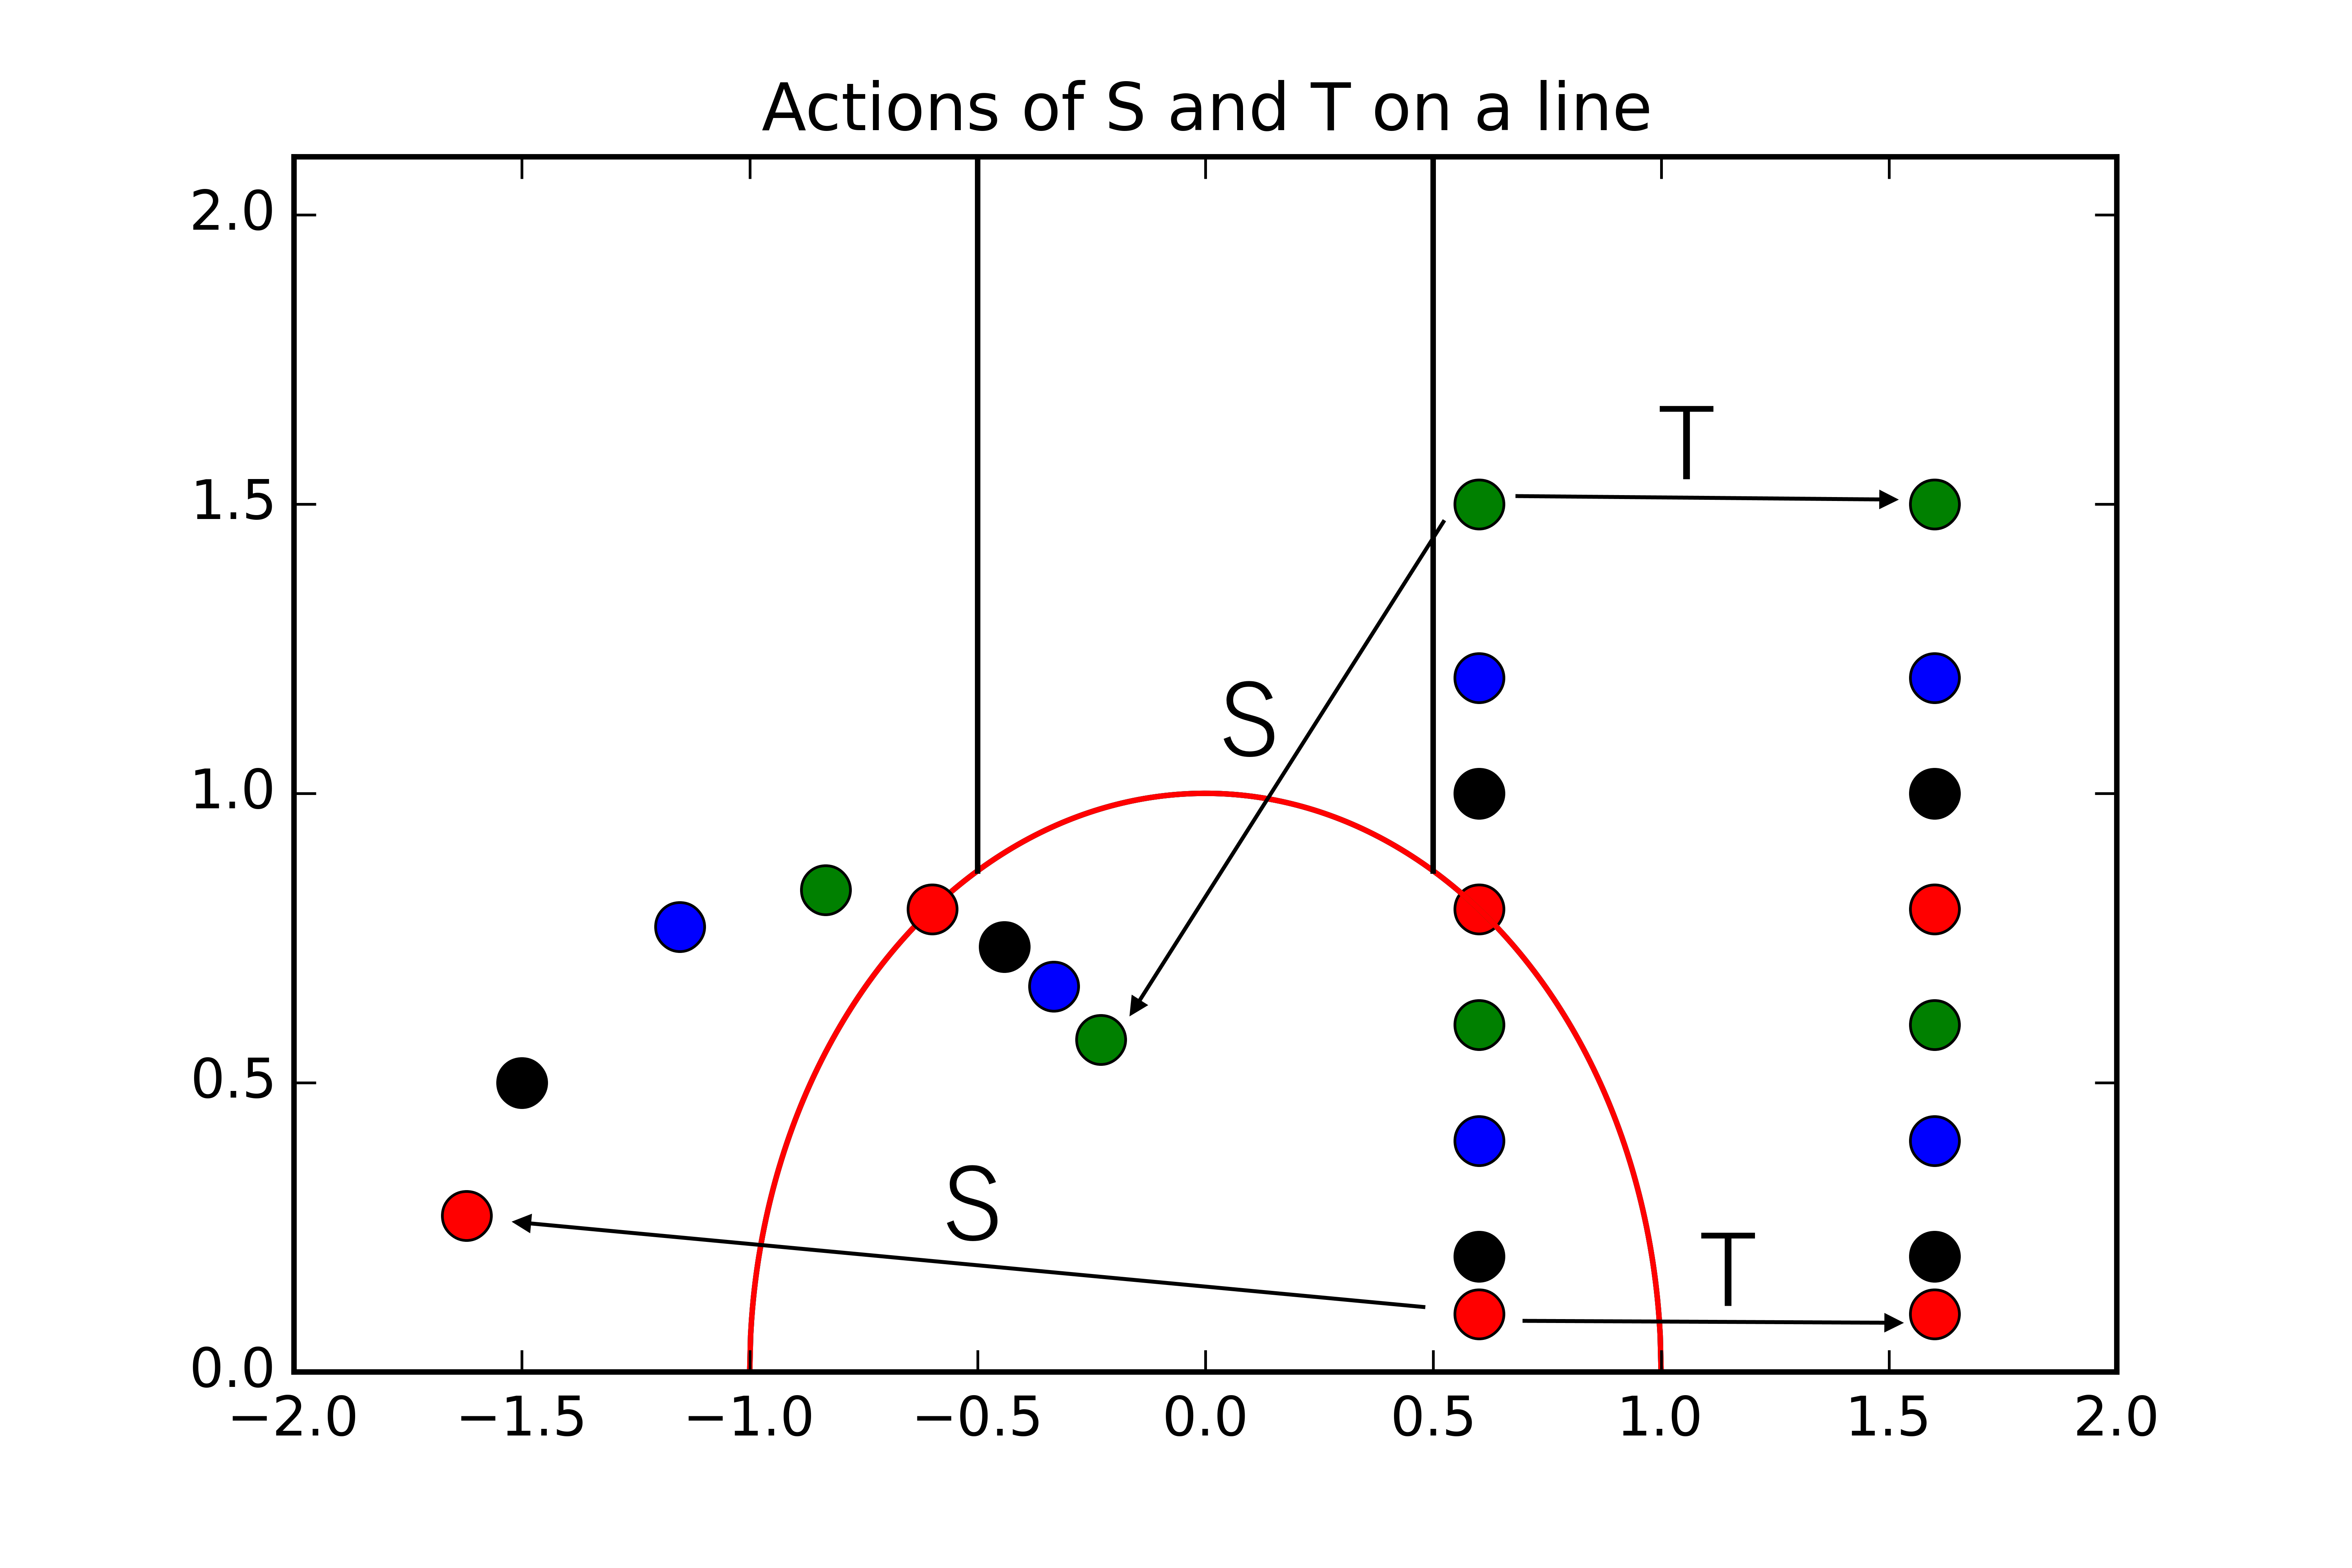
\includegraphics[height=2in]{ActionSTLine}
    \else
      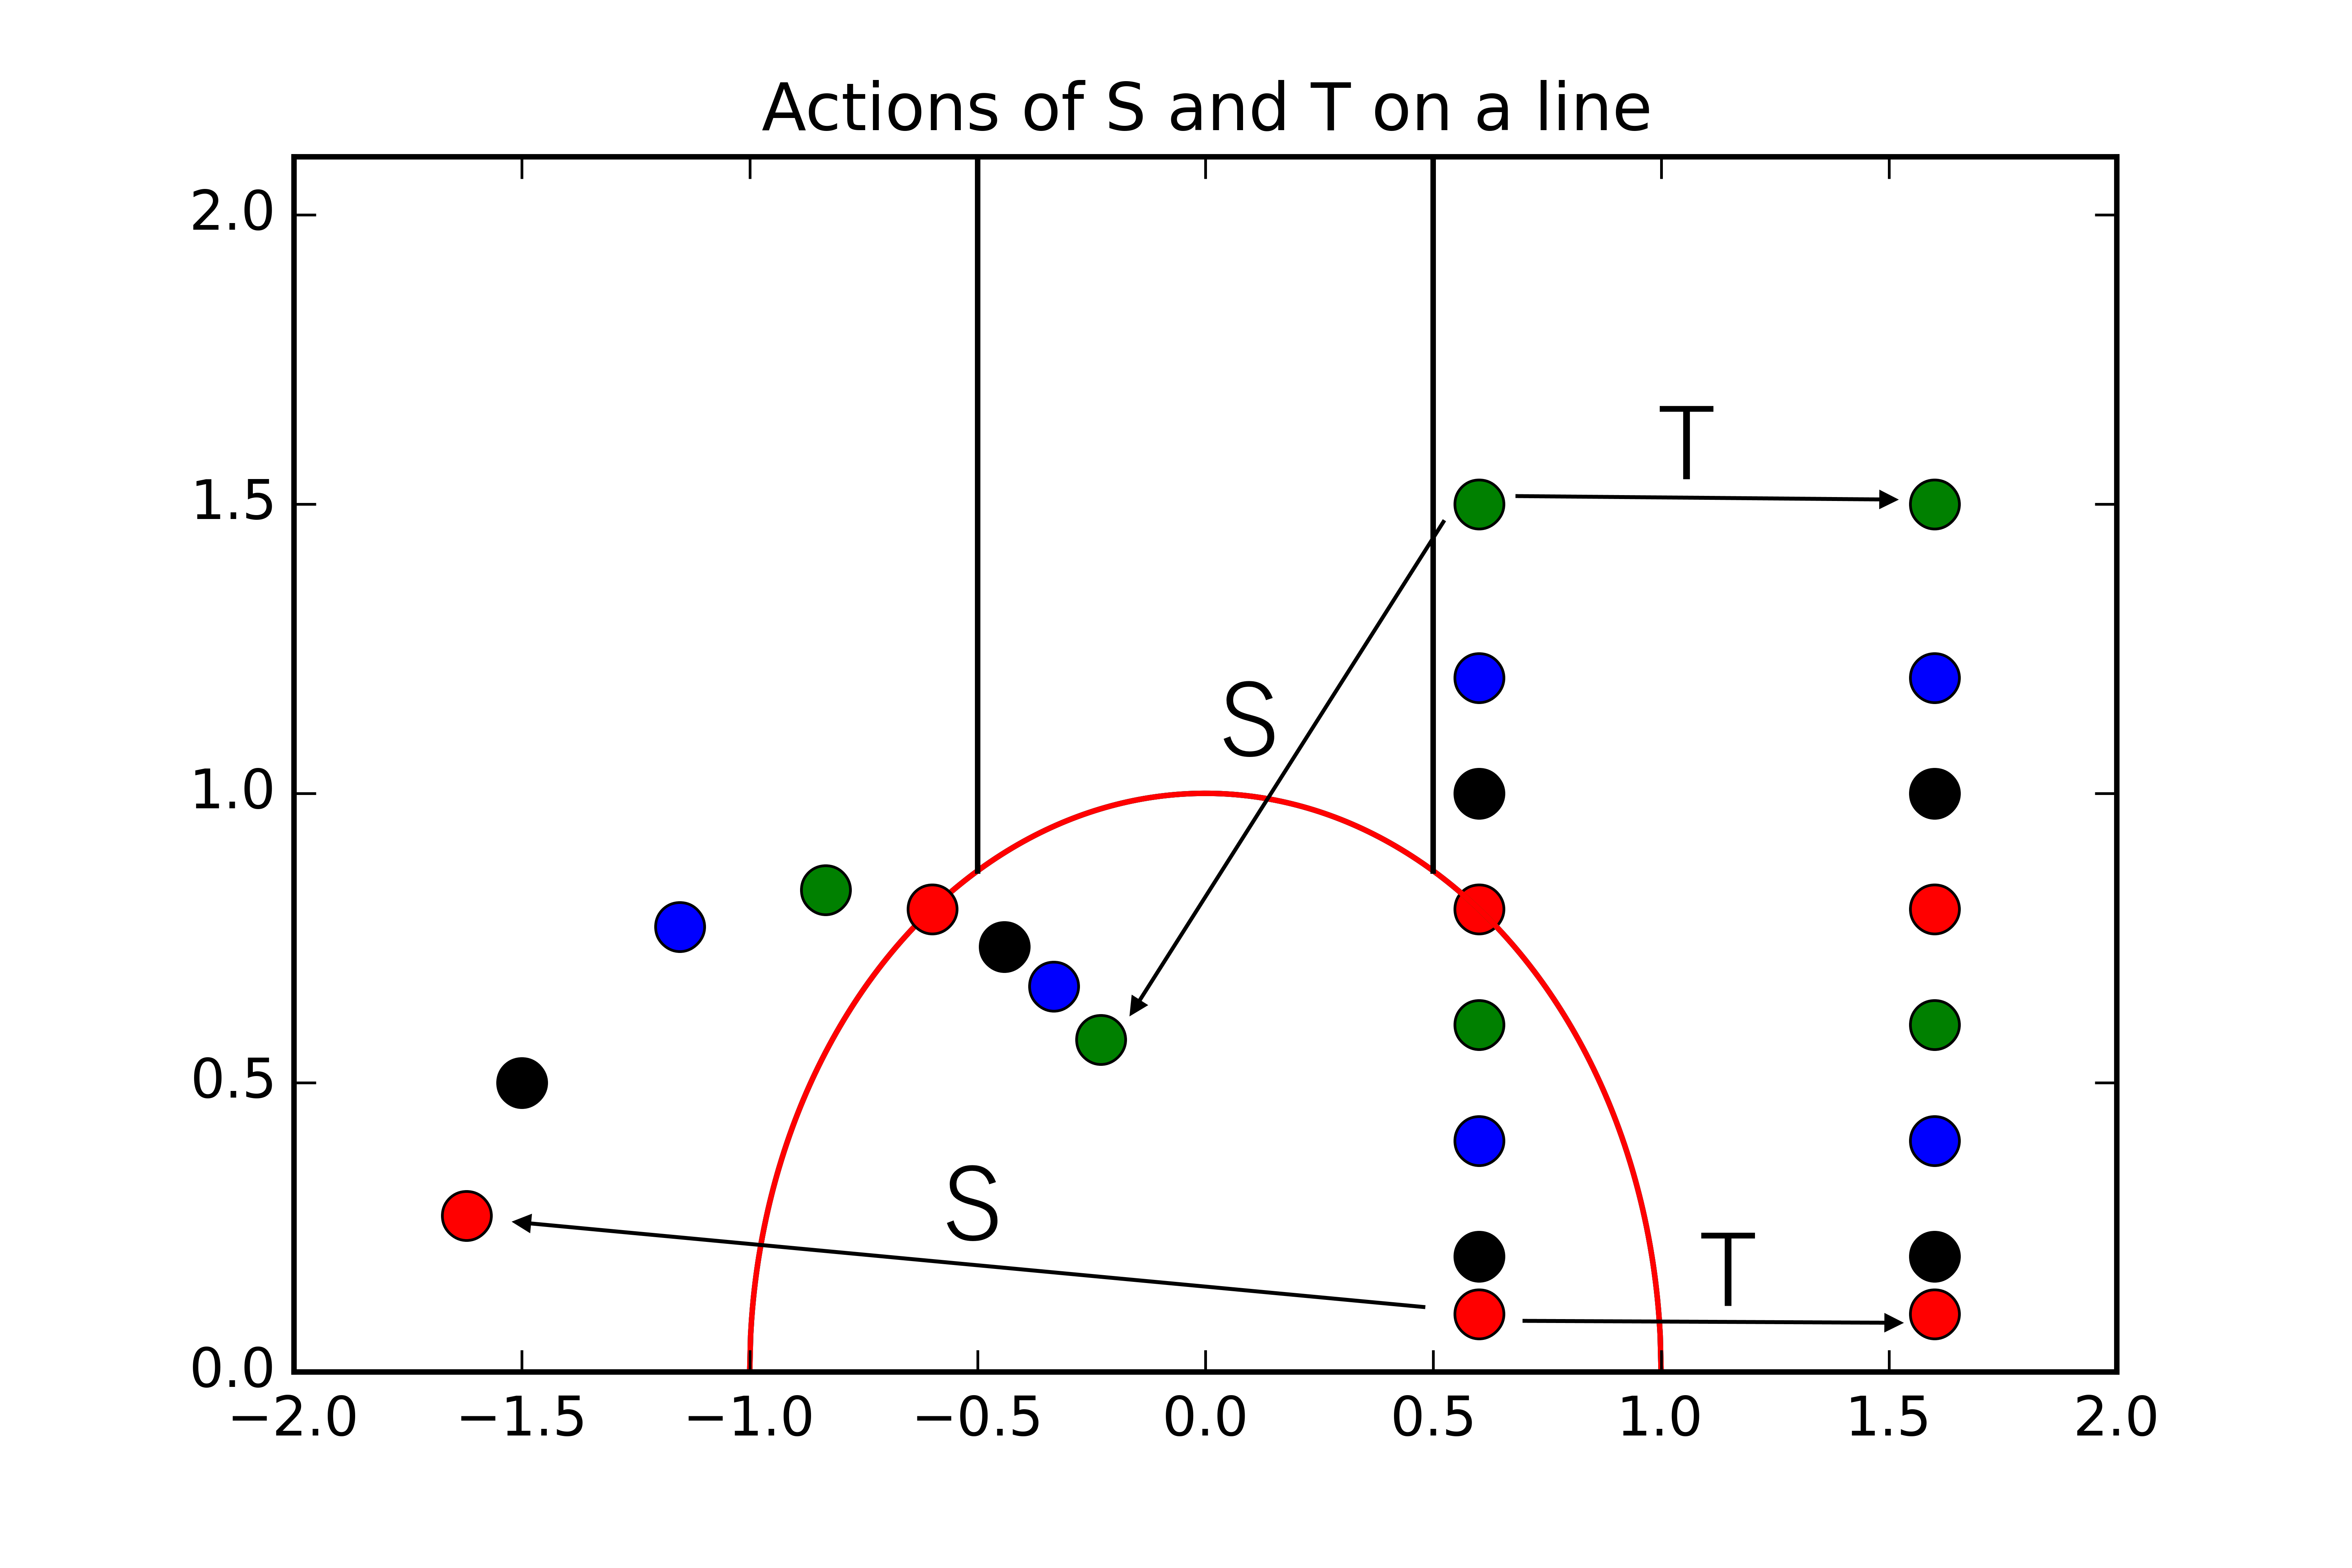
\includegraphics[bb = 92 86 545 742, height=6in]{ActionSTLine}
    \fi
    \caption{Example: action of $S$ and $T$}
    \label{fig:actionST}
  \end{center}
\end{figure}

\begin{figure}[!htbp]
\centering
\begin{subfigure}{.5\textwidth}
  \centering
      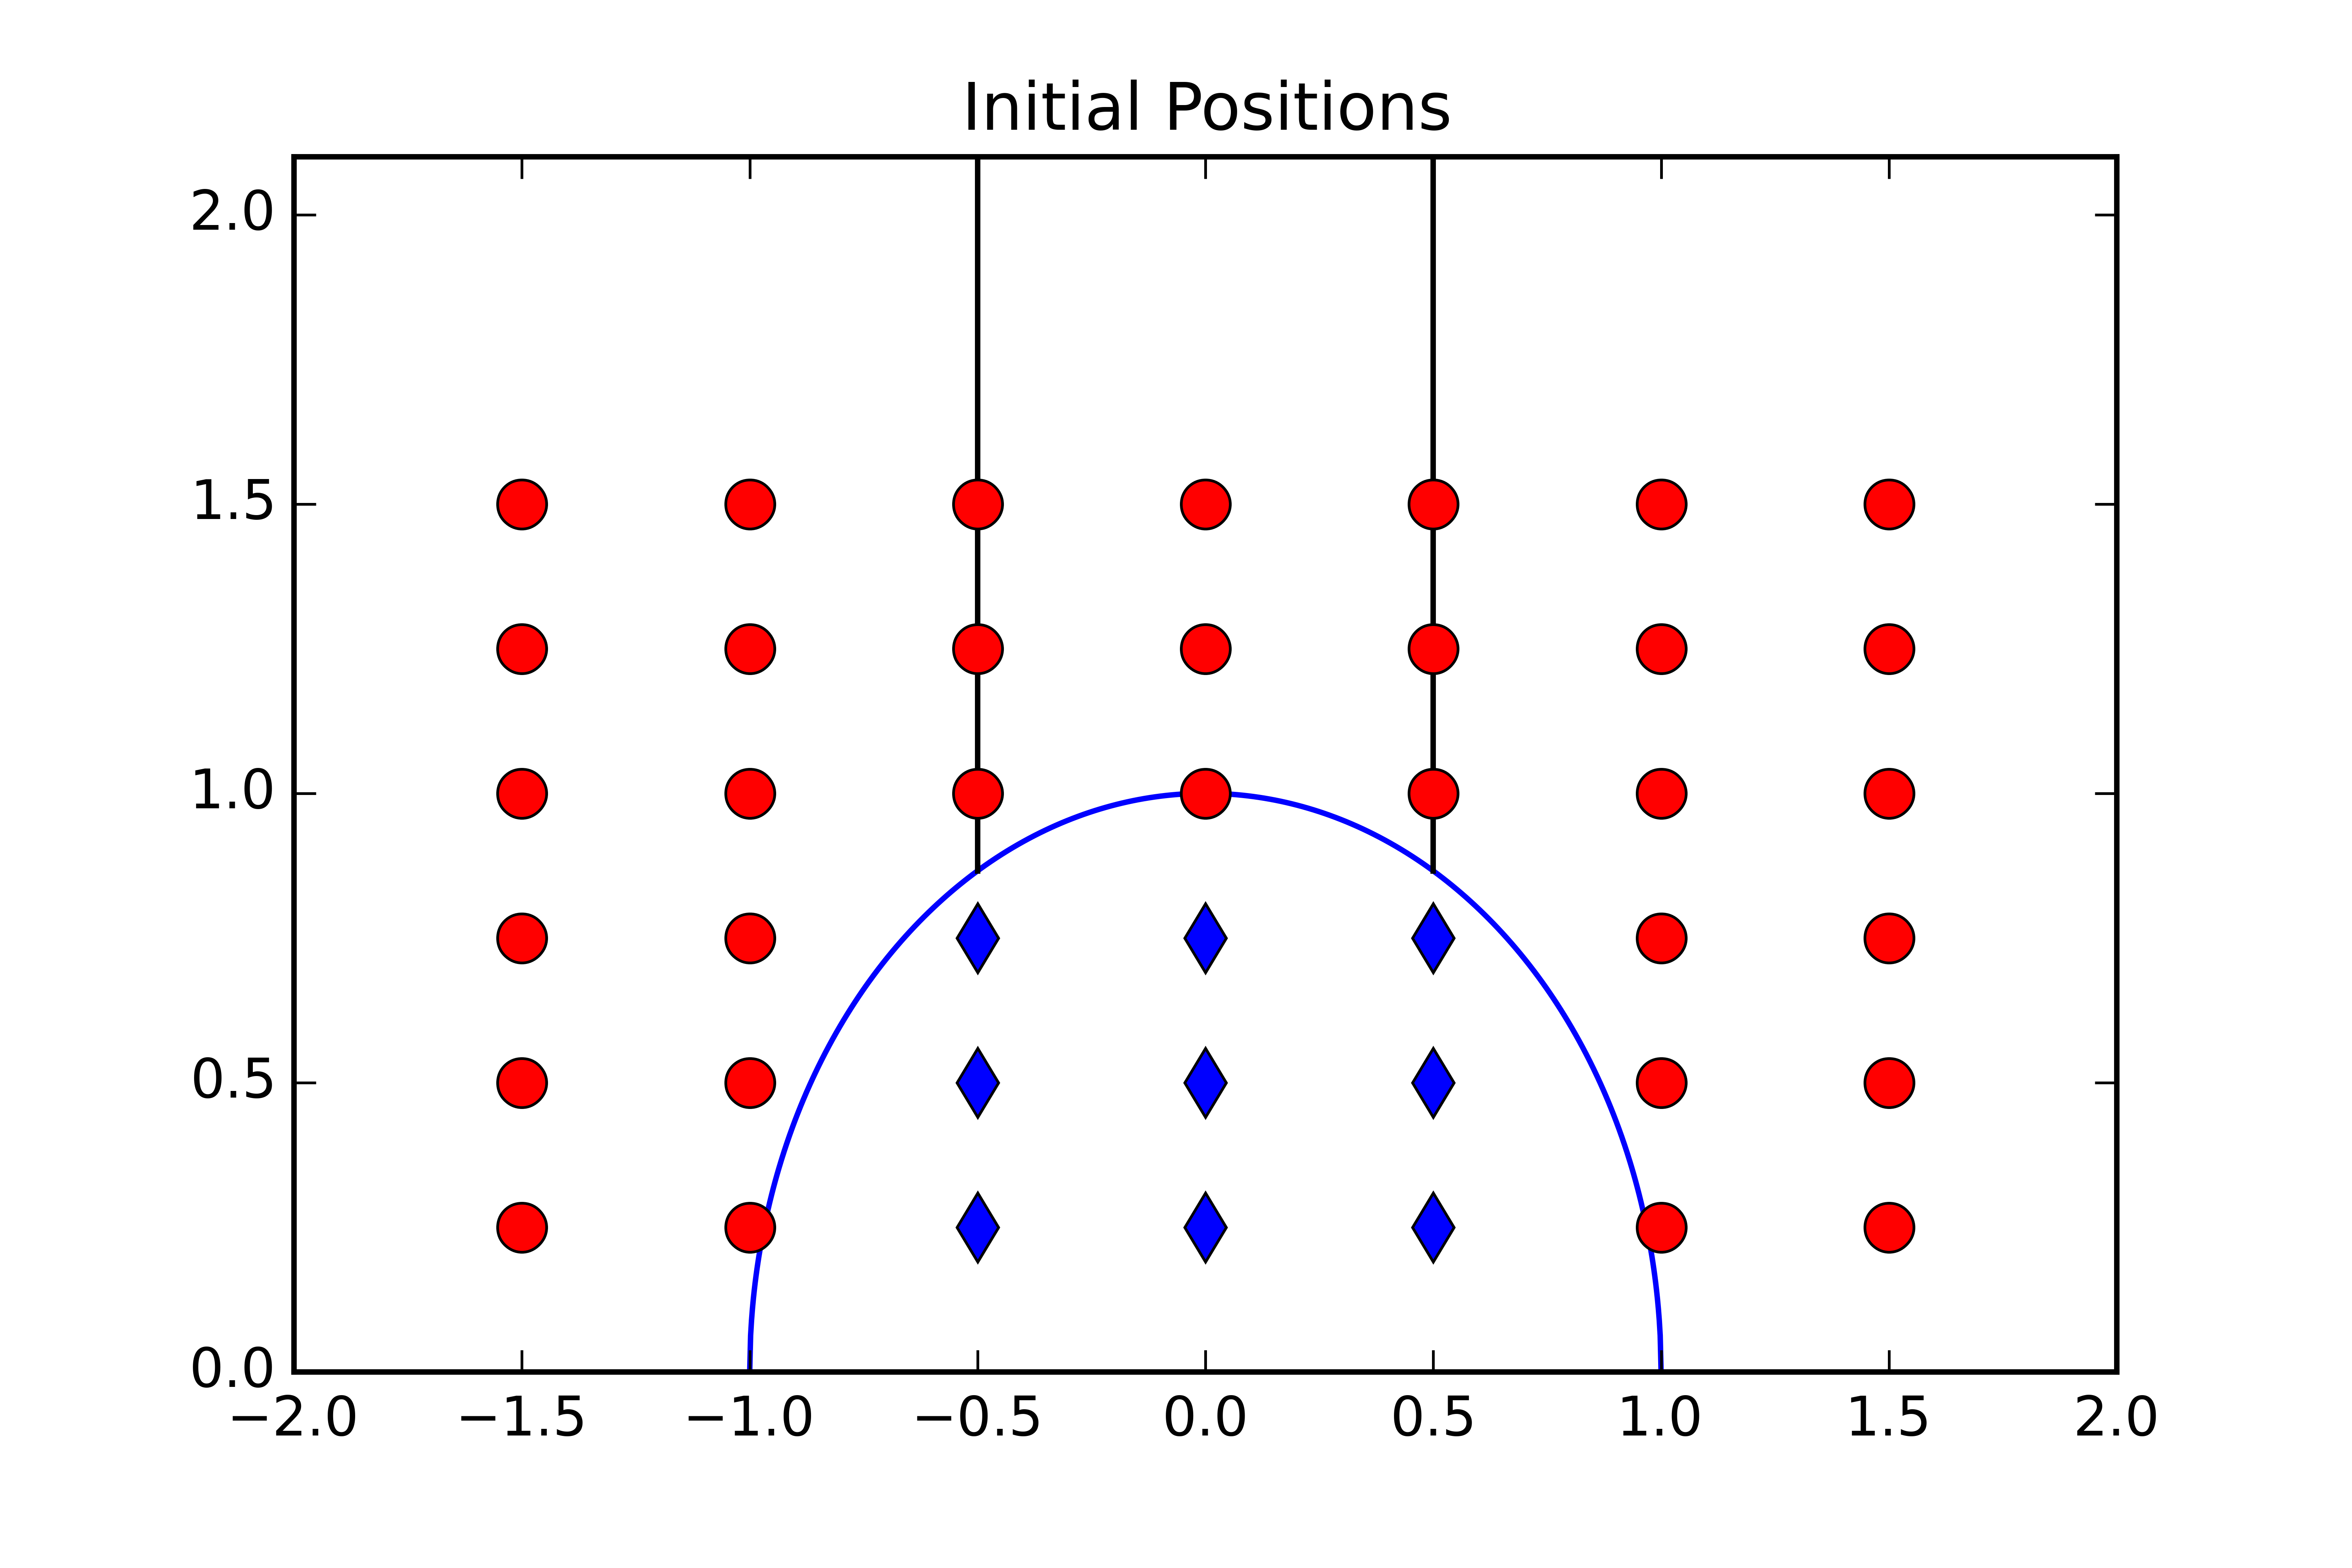
\includegraphics[height=2in]{SGridTransform-0}
  \caption{Before}
  \label{fig:beforeS}
\end{subfigure}%
\begin{subfigure}{.5\textwidth}
  \centering
      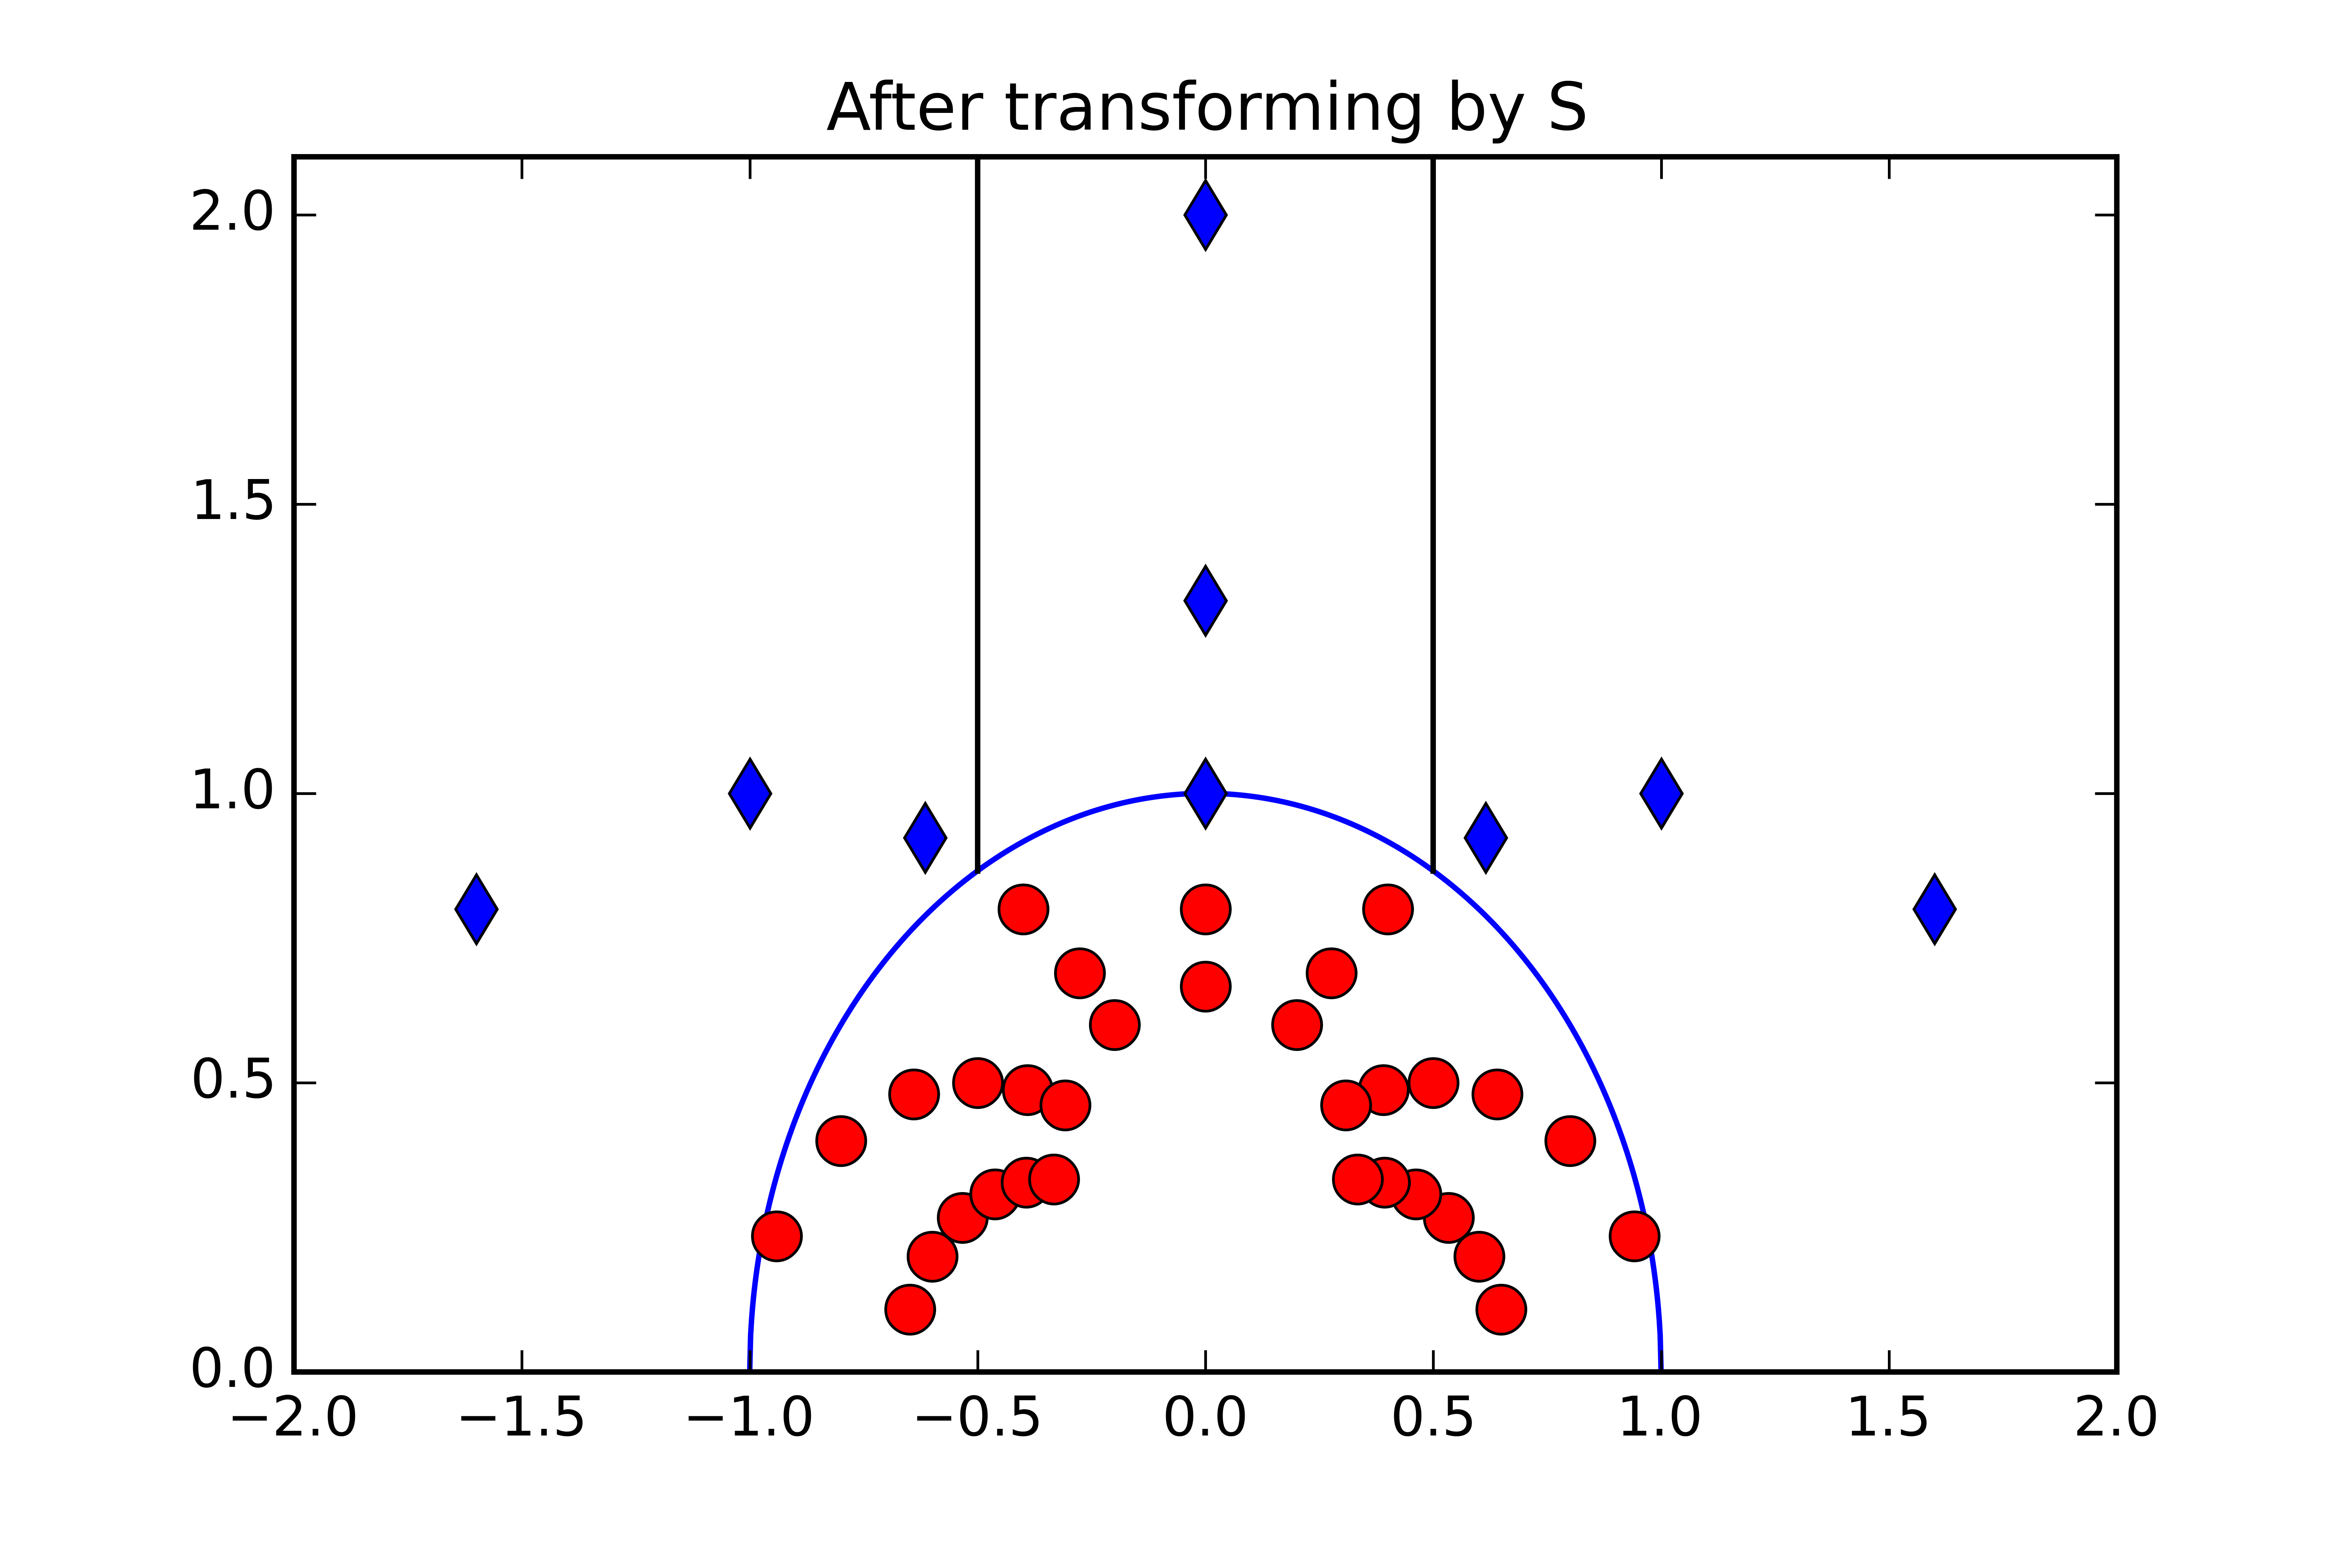
\includegraphics[height=2in]{SGridTransform-1}
  \caption{After action by $S$}
  \label{fig:afterS}
\end{subfigure}
\caption{Example: Action on grid of points }
\label{fig:actionS}
\end{figure}

We can define a group action of $\sltz$ on the upper half plane $\mathcal{H}$ through Möbius transformations. \\
Let $ A = \abcd \in \sltz$ and let $z \in \mathcal{H}$, we define the group action $A \cdot z = h(A)(z) = \frac{az +b}{cz +d}$.\\
We can check this satisfies the definition of group action given in \ref{def:groupAction}.
This group action satisfies associativity: if we have $A, B \in \sltz$, then for $z \in \mathcal{H}$, 
\begin{align*}
A \cdot (b \cdot z)  = A \cdot (h(B)(z)) & = h(A)(h(B)(z))  \\
 \quad & = (h(A)h \circ (B))(z)  \\
\small{(h \text{ is a homomorphism})} \quad \quad & = h(AB)(z) = (AB) \cdot z
\end{align*}

The second condition of being a group action is also satisfied, $I_2 \cdot (z) = z$ for all $z \in \mathcal{H}$.\\
\\


From now on we often refer to $\sltz$ as $\Gamma$. 

\begin{definition}
Let $\Gamma'$ be a subgroup of $\Gamma$. Two points $z_1, z_2$ in $\mathcal{H}$ are said to be $\Gamma'$ equivalent if they are in the same $\Gamma'$-orbit. That is to say there exists a $\gamma \in \Gamma'$ such that $\gamma z_1 = z_2$. 
\end{definition}
Note: Recall the notation $\gamma z$ for $\gamma \in \Gamma$ and $z \in \mathcal{H}$ means the group action of $\gamma$ on $z$, i.e $h(\gamma)(z)$. 
\begin{definition}
A fundamental domain $\mathcal{F}$ for a subgroup $\Gamma'$ of $\Gamma$ is a closed subset of $\mathcal{H}$ such that 
\begin{enumerate}
\item $ \cup_\gamma \Gamma' \gamma(\mathcal{F}) =\mathcal{H}$,
\item the images $\gamma(\text{int}(\mathcal{F}$)) are pairwise disjoint; that is $\gamma_1(\text{int}(\mathcal{F})) \cap \gamma_2(\text{int}(\mathcal{F})) = \emptyset$ if $ \gamma_1, \gamma_2 \in \Gamma', \gamma_1 \neq \gamma_2$. \\
( Here int($\mathcal{F}$) denotes the \textit{interior} of $F$, the largest open set contained inside $\mathcal{F}$ ). 
\end{enumerate}
\end{definition}

Restating the above definition gives, a closed subset of $\mathcal{H}$, $\mathcal{F}$, is a fundamental domain for $\Gamma'$ if 
\begin{enumerate}
\item The orbit of every $z \in \mathcal{H}$ contains some point in $\mathcal{F}$ 
\item No two distinct points in the interior of $\mathcal{F}$ are contained in the same orbit.
\end{enumerate}
We say that the images of $\mathcal{F}$ under $\Gamma'$ \textit{tessellate} $\mathcal{H}$.

\begin{example}\label{ex:fundamentalDomainT}
Consider the subgroup $\langle T \rangle$ of $\Gamma$, which has corresponding subgroup $\{\gamma_n \, \vert \, \gamma_n(z) = z+n, \, n \in \mathbb{Z}\}$ in $\mobh$ under the image $h \, : \, \Gamma \rightarrow \mobh$. The set $\mathcal{F} = \{ z \in \mathcal{H} \vert 0 \leq Re(z) \leq 1 \}$ is closed. Let $z \in \mathcal{H}$, then $ \leq n Re(z) < n+1$ for some $n \in \mathbb{N}$. We consider $Re(\gamma_{-n}(z)) = Re(z - n) = Re(z) - n$, which lies in the interval $ 0 \leq Re(\gamma_{-n}z) < 1$, so $\gamma_{-n}(z) \in \mathcal{F}$. \\
Next suppose we have $z_1, z_2 \in$ int($\mathcal{F}$), in particular $ 0 \leq Re(z_1) < Re(z_2) \leq 1$, and suppose $\gamma_n z_1 = z_2$ for some $n$. The bounds on $z_1$ and $z_2$ mean that the maximum distance is $1$ and so $\gamma_n = \gamma_1 = z + 1$. The only two points distance $1$ in the interval $[0,1]$ are $0$ and $1$, so $Re(z_1) = 0$ and $Re(z_2) = 1$. So they do not lie in the interior of $\mathcal{F}$. \\
Hence $\mathcal{F}$ is a fundamental domain for $\langle T \rangle$. 



\end{example}

\begin{example}\label{ex:fundamentalDomainS}
The set $\mathcal{F} = \{z \in \mathcal{H} \, \vert \, \vert c \vert \leq 1\}$ is a fundamental domain for the group $\Gamma' = \langle S \rangle$. The subgroup of $\mobh$ corresponding to $\Gamma'$ is $\{z, -1/z\}$.\\
Let $z$ be a point in $\mathcal{H}$ that is not in $\mathcal{F}$, then $-1/z$ is in the fundamental domain. \\
If $z_1, z_1$ are two distinct $\Gamma'$ equivalent points then we must have $-1/z_1 = z_2$, this occurs only when $\vert z_1 \vert = \vert z_2 \vert = 1$, i.e only on the boundary of $\mathcal{F}$.
\end{example}


\subsection{Geometric proof that $S,T$ generate $\sltz$}

The geometric proof of Theorem \ref{thm:STGenerateSLTZ} is done in two main steps. First we construct a fundamental domain for $\Gamma$ using the action of $G: = \langle S, T \rangle \subset \Gamma$, next we use it to show $G \supset \Gamma$ and so $G = \Gamma$. 
\\ 
The actions of $S, T$, along with the fundamental domains of $\langle T \rangle$ and $\langle S \rangle$ give an idea of one possible fundamental domain for $\Gamma$.

\begin{lemma}\label{lem:gorbitfund}
Every element $z\in \mathcal{H}$ has an element of it's G-orbit in $\mathcal{F} = \{z \in \mathcal{H} \, | \, -1/2 \leq z \leq 1/2 \, |z| \geq 1  \}$.
\end{lemma}
(Note: This implies every element of $Z \in \mathcal{H}$ has an element of it's $\Gamma$-orbit in $\mathcal{F}$, since $G \subset \Gamma$).

\begin{proof}

Let $g  = \abcd \in G$, let $z \in \mathcal{H}$. Then as we've observed in \ref{eqn:imaginaryMobius},
$$ Im(gz) = \frac{Im(z)}{{\vert cz +d \vert}^2}.$$
Geometrically since $c,d$ are integers the points $cz+d$ lie on the lattice generated by $1$ and $z$. 
This means that there is no infinite decreasing sequence 
$$\vert c_1z + d_1  \vert > \vert c_2z + d_2  \vert > \vert c_3z + d_3  \vert  > \cdots  \text{ for integers } c_i,d_i.$$ 
This is since for any $\lambda \in \mathbb{R}, c \in \mathbb{Z}$ we could find $d$ sufficiently large such that $\vert cz + d \vert > \lambda$ and $\vert cz -d \vert > \lambda$. So given $c \in \mathbb{Z}$ there are finitely many $d_i \in \mathbb{Z}$ such that $\vert cz + d_i \vert < \vert c_1z + d_1  \vert$. For each such $d_i$ there are finitely many $c_i$ that satisfy $\vert cz + d_i \vert < \vert c_1z + d_1  \vert$. Thus the sequence is finite and must terminate.
\\
It implies there is no infinite increasing sequence 
$$ Im(g_1z)  < Im(g_2z) < \cdots \text{ for } g_i\in G$$

This means that the following procedure will eventually move every element $z$ in $\mathcal{H}$ in to the fundamental domain $\mathcal{F}$.\\
Let $z = z_0$.
\begin{enumerate}[(i)]
\item Translate $z_0$ to $z_1$ by $T^n$ such that $| Re(T^nz)| \leq 1/2$ for some $n \in \mathbb{N}$. ( We showed this was possible, for a translated domain, in Example \ref{ex:fundamentalDomainT}).
\item If $z_1$ lies in the fundamental domain we are done. If not then it must lie inside the unit circle with $|z_1| < 1$, so we invert by $S$ to get $z_2 = S(z_1)$. Observe that 
$$ Im(z_2) = Im(Sz_1) = \frac{Im(z_1)}{{|z_1|}^2} > Im(z_1) \text{ since } |z_1| < 1.$$
\item If $z_2$ is in the fundamental domain we are done, otherwise let $z_0 = z_2$ and return to the first step.
\end{enumerate}
From this procedure we get a sequence 
$$Im(z) < Im(ST^{n_1}z) < Im(ST^{n_2}ST^{n_1}z) < \cdots,$$
we noted already that such a sequence must be finite, so eventually the process will terminate.
\end{proof}

An example of this procedure applied to multiple points is given in Figure \ref{fig:procedure}.
\begin{figure}[!htbp]
\begin{tabular}{cc}
  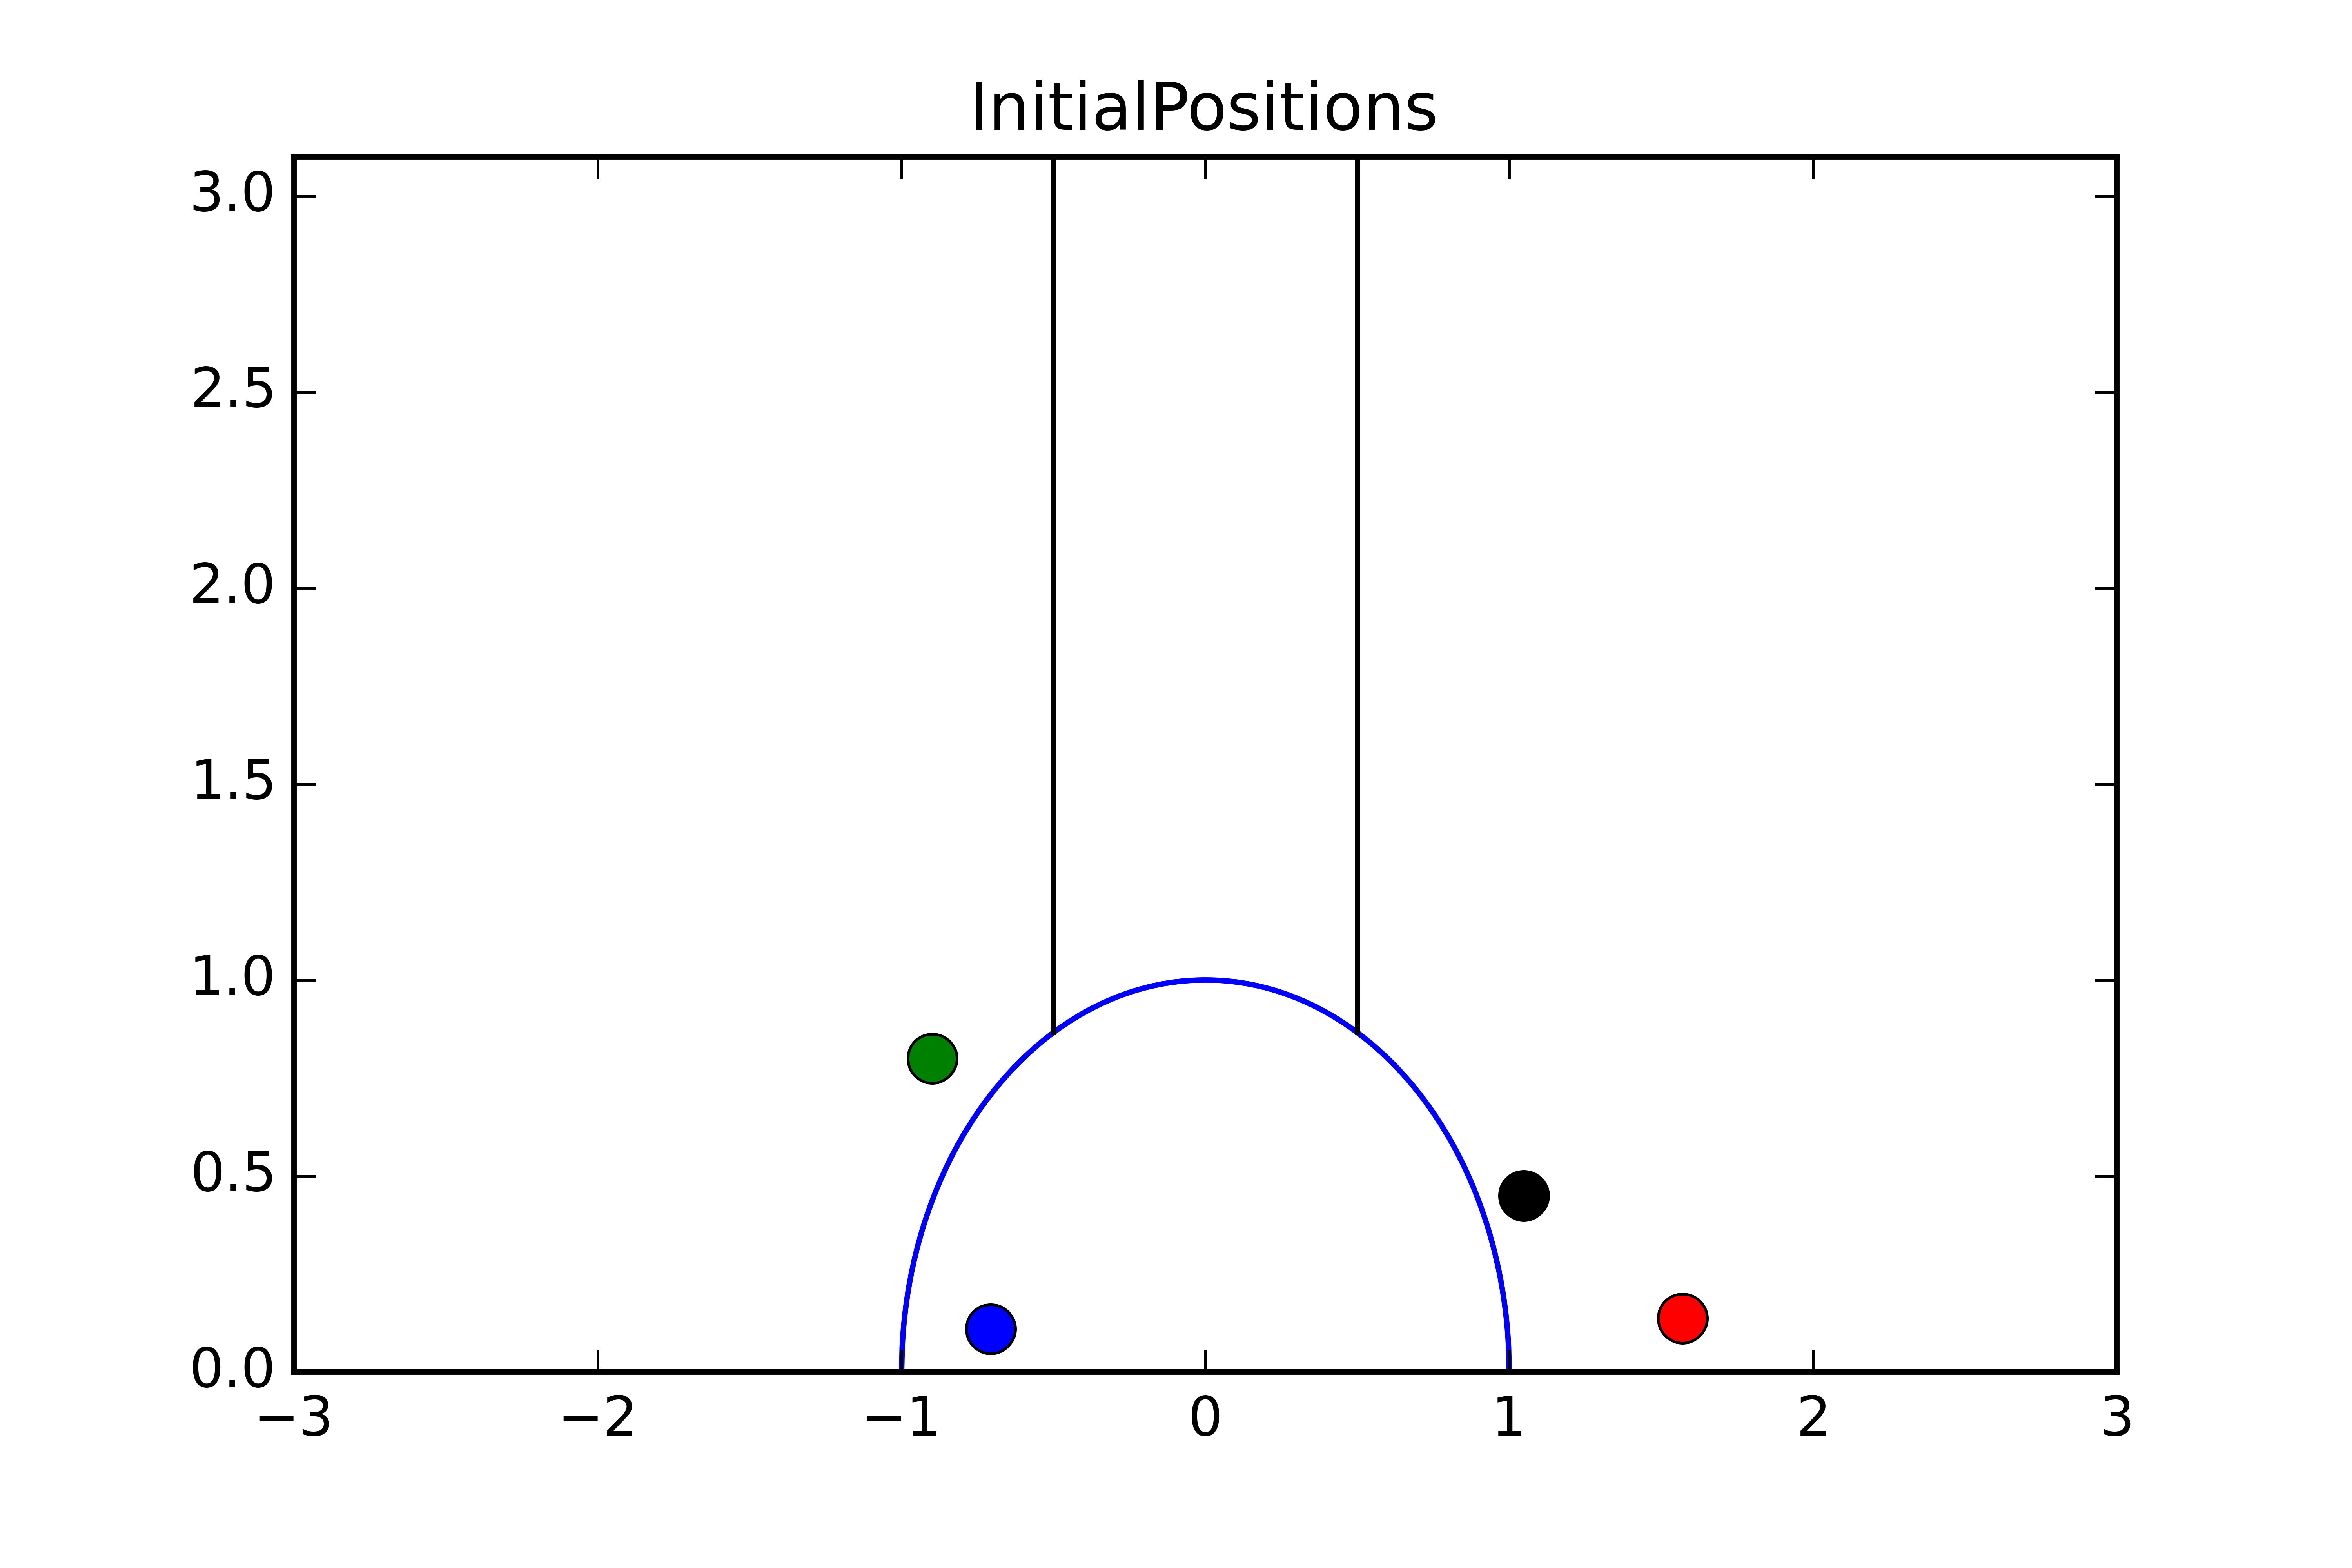
\includegraphics[width=65mm]{FundDomain-0} &   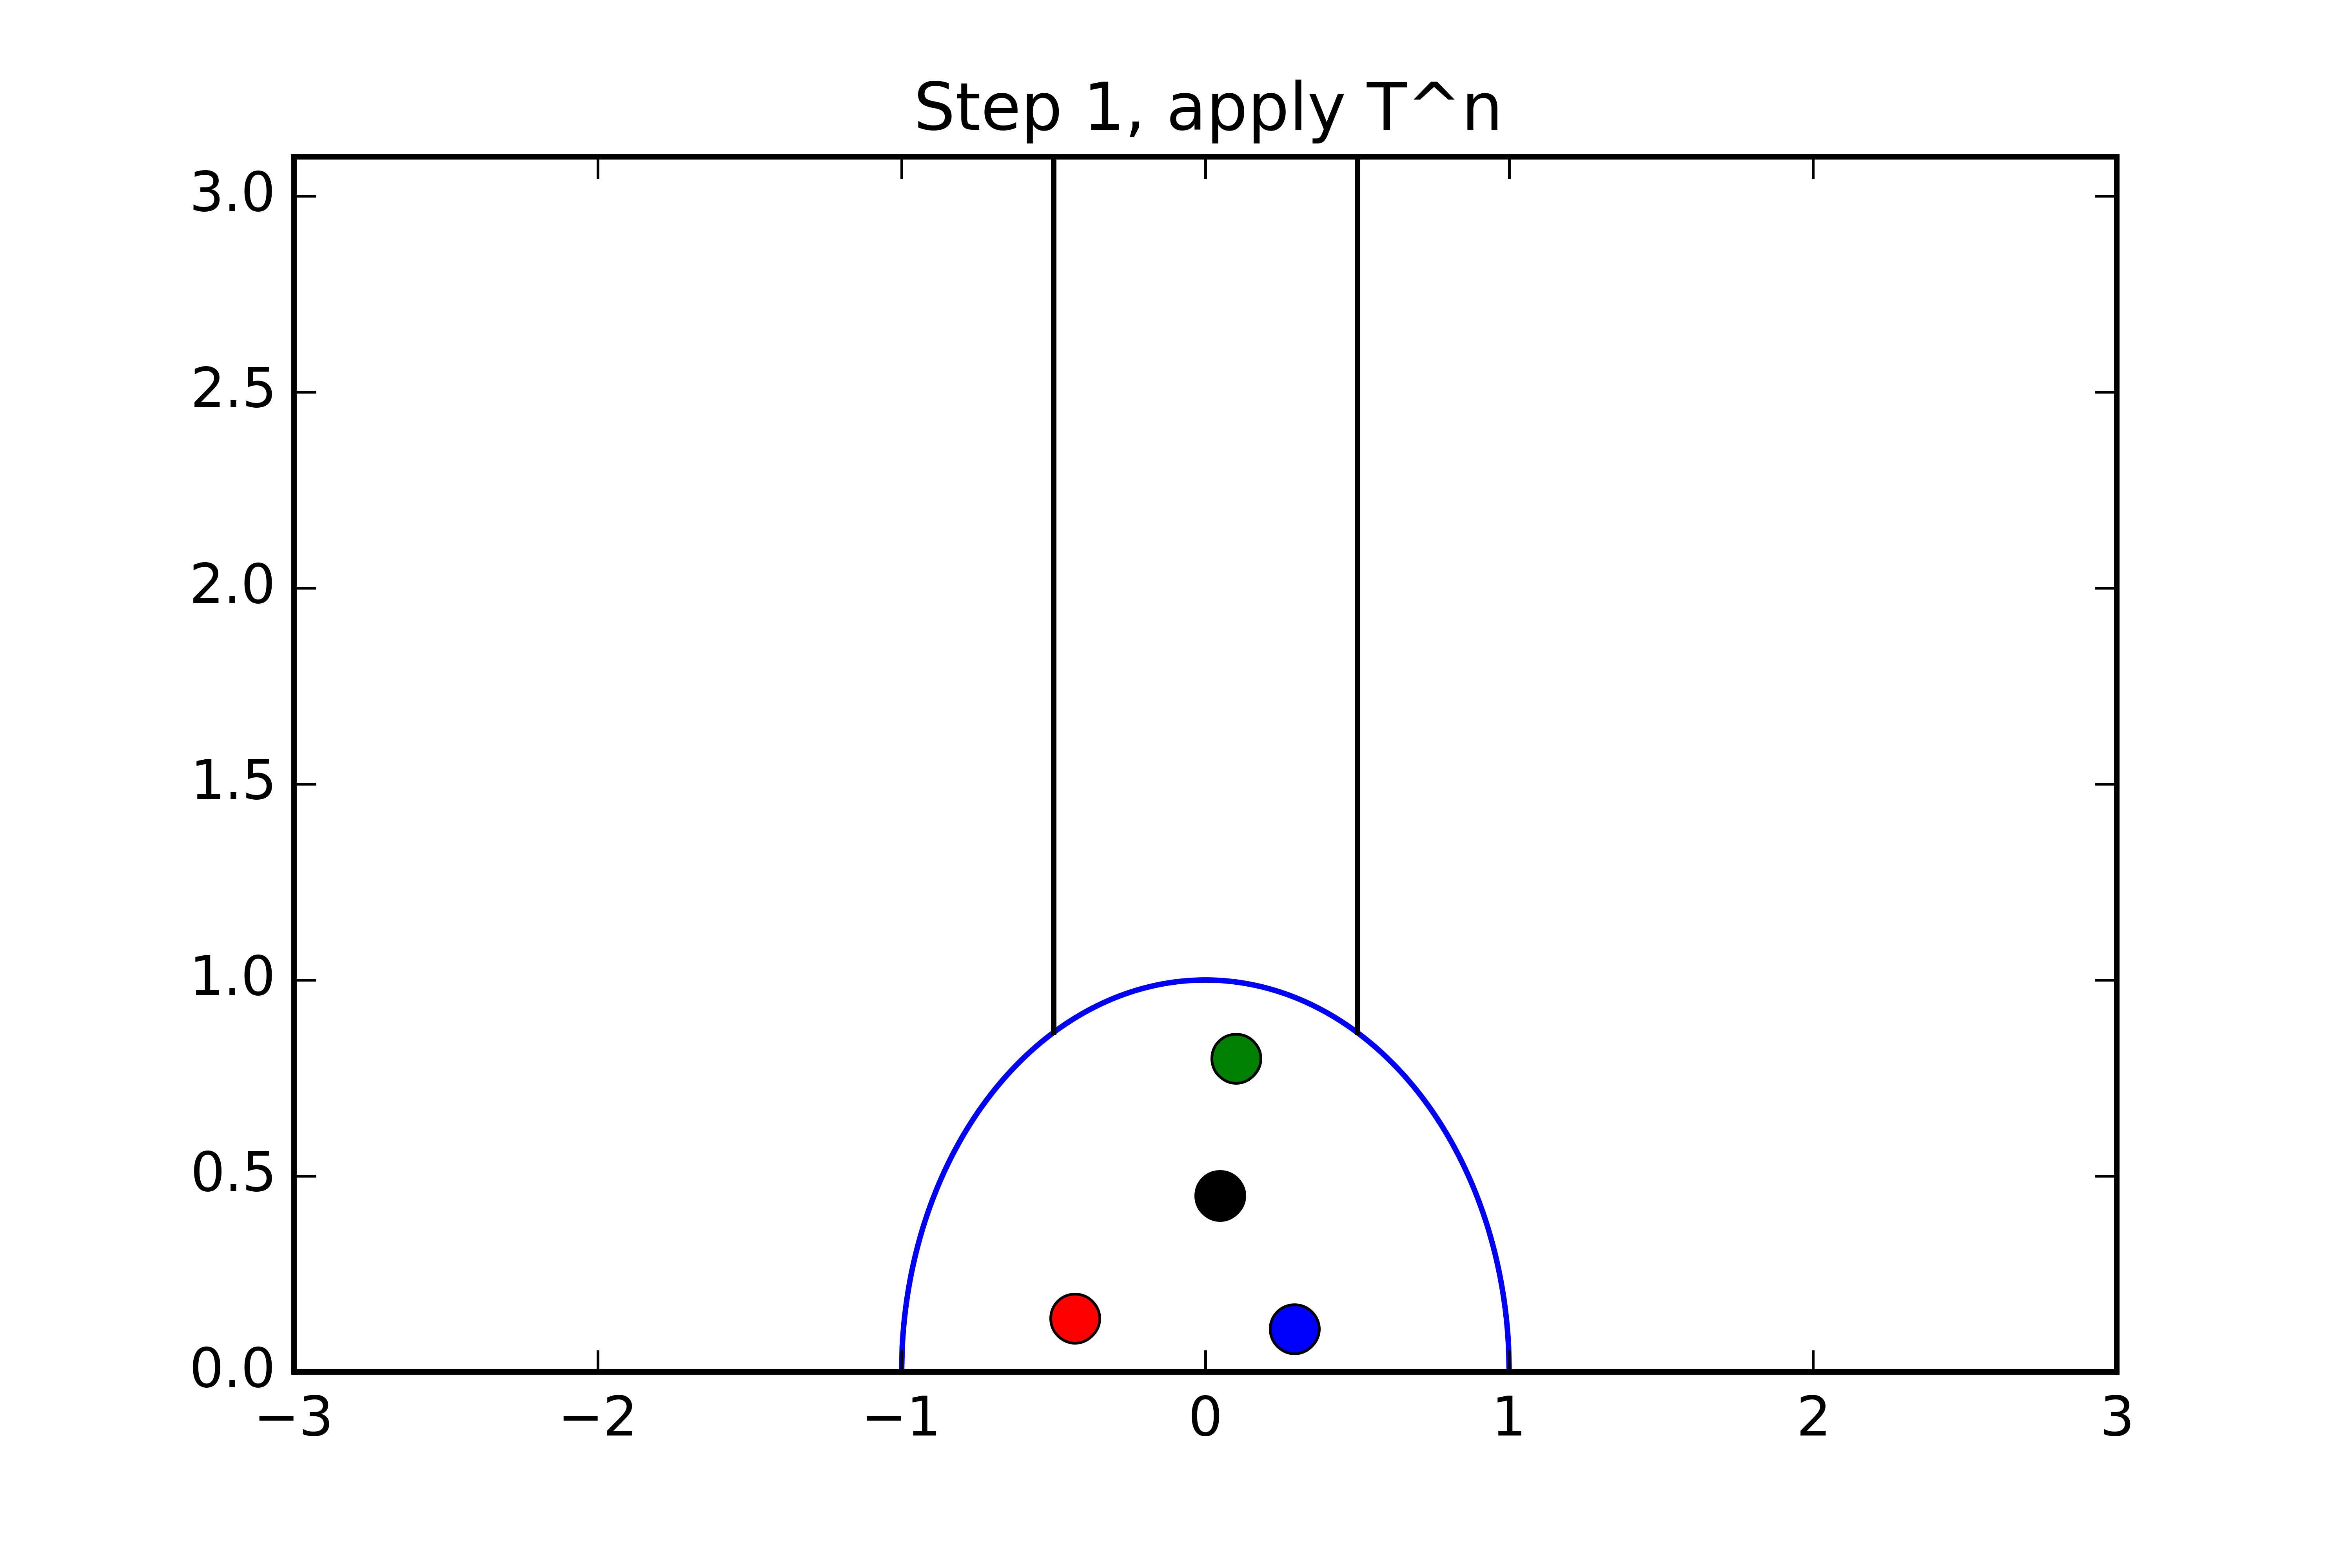
\includegraphics[width=65mm]{FundDomain-1} \\
(a) Initial & (b) Apply $T^n$ \\[6pt]
 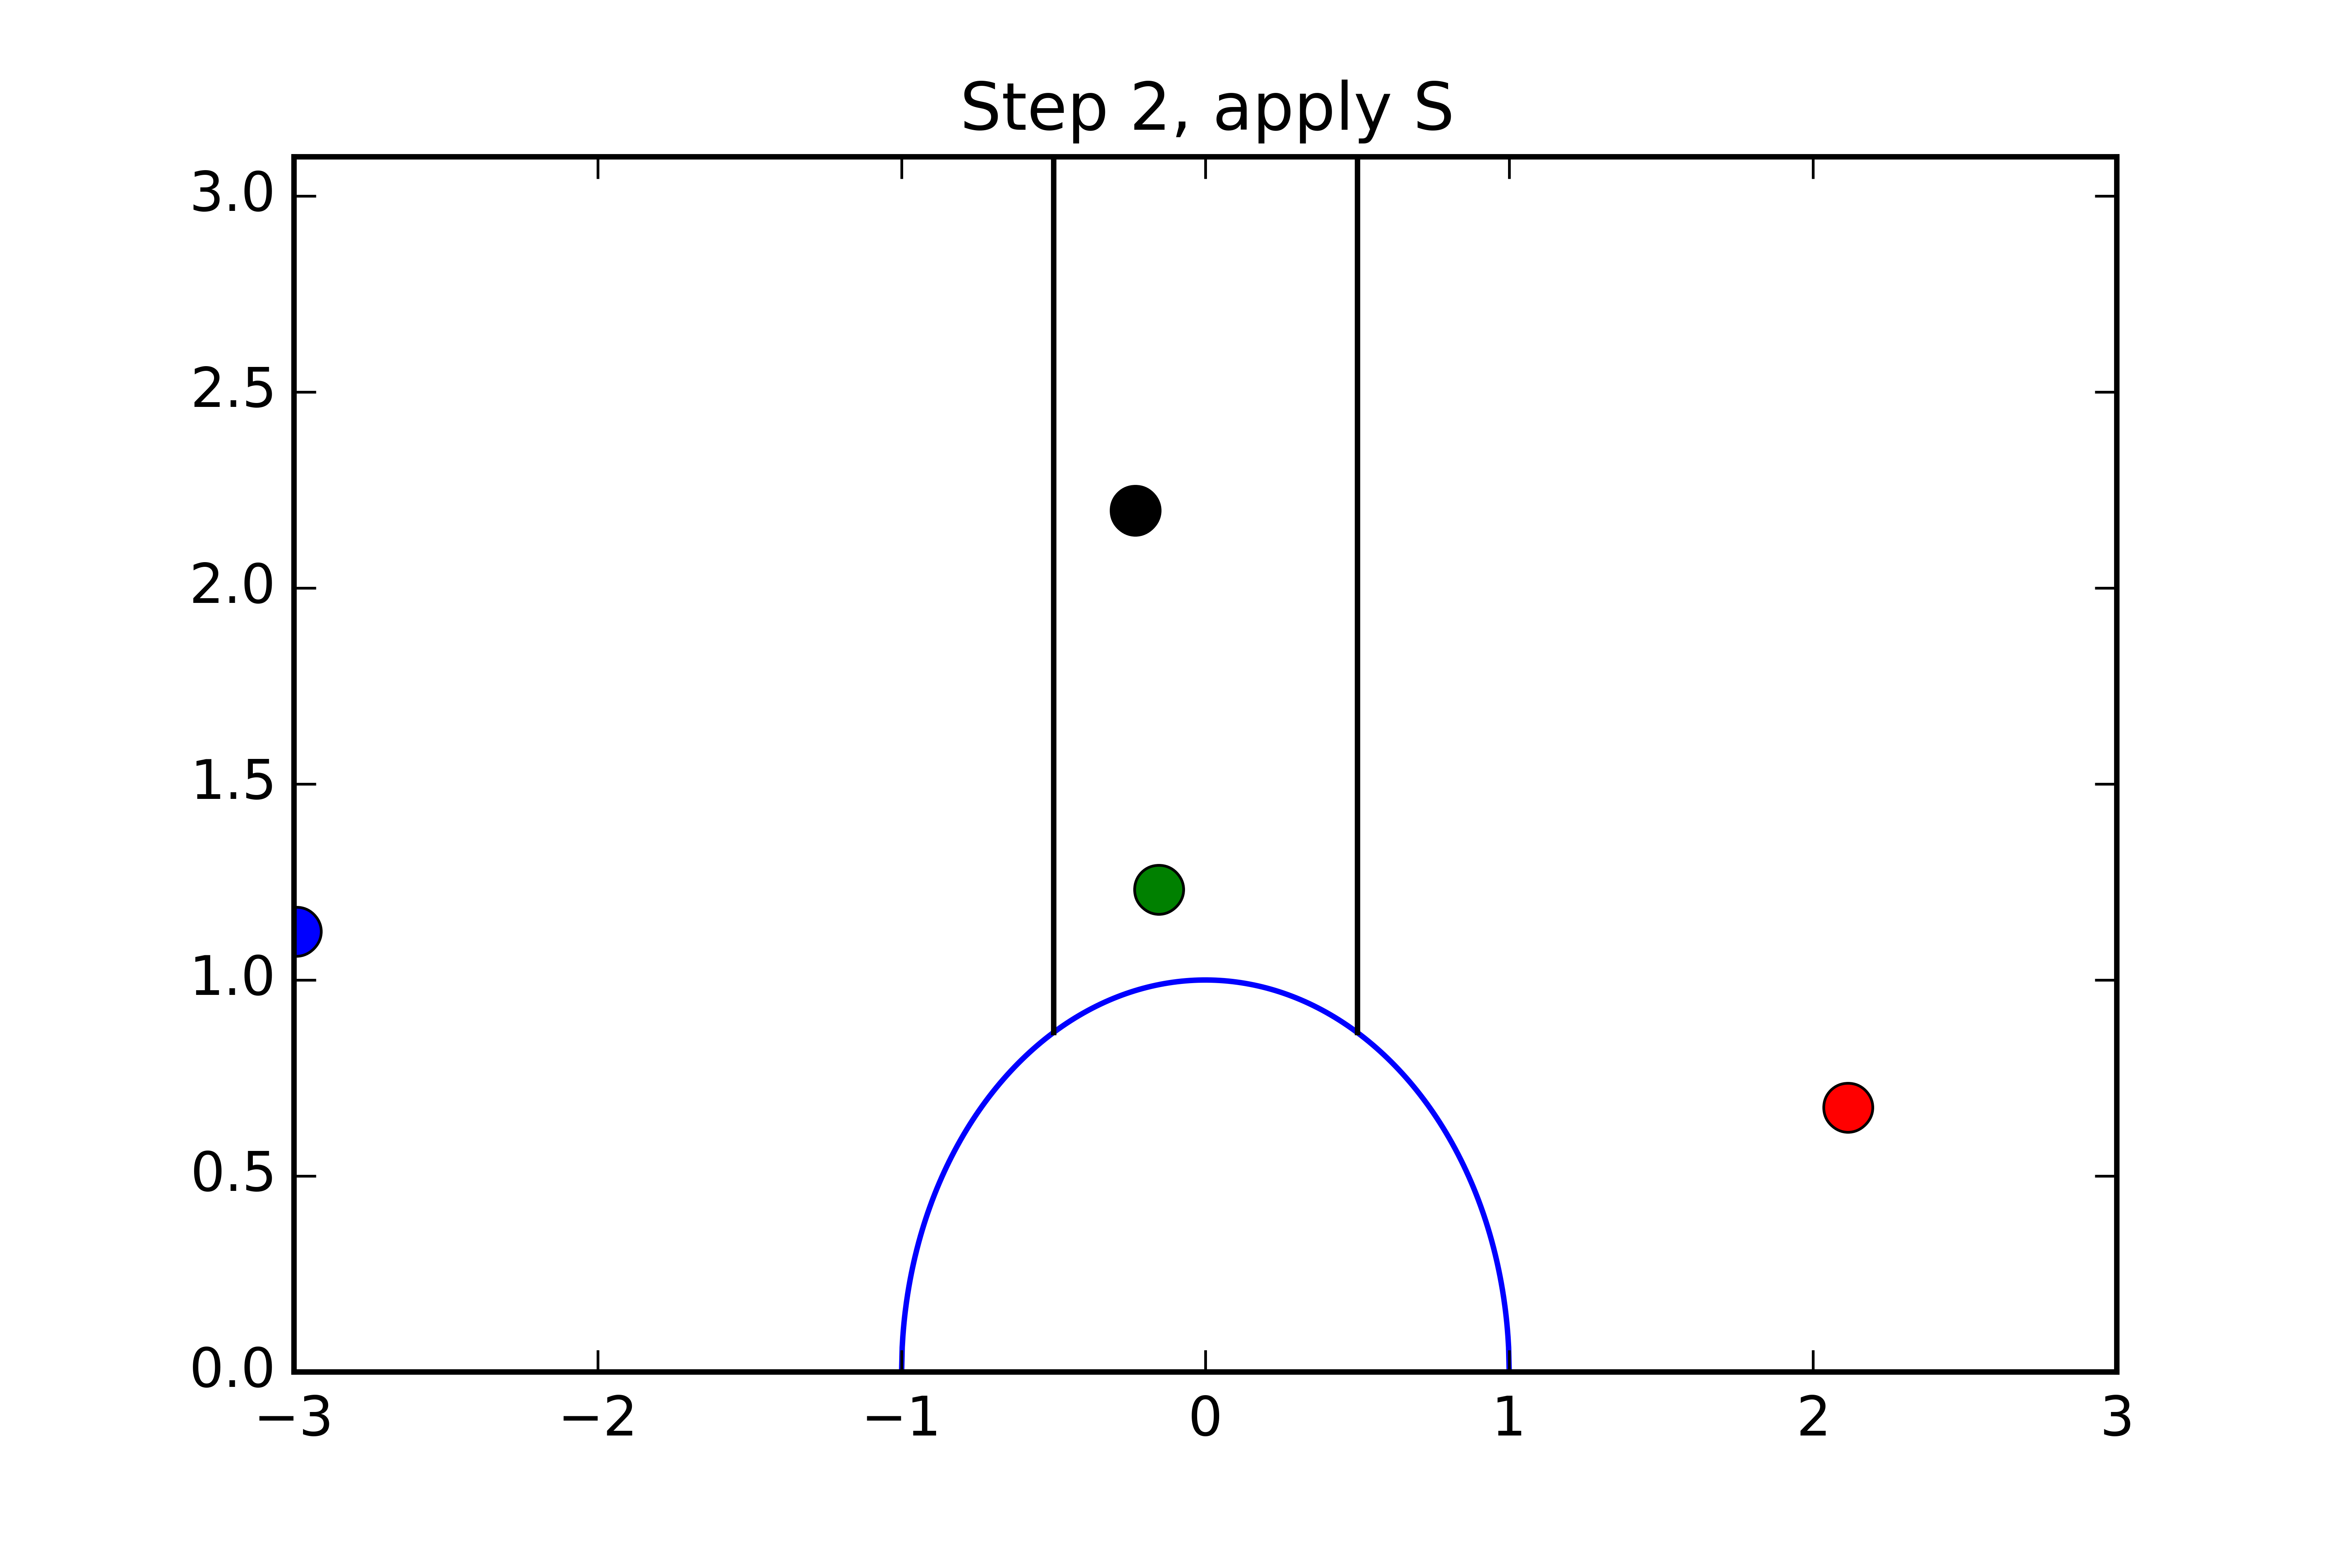
\includegraphics[width=65mm]{FundDomain-2} &   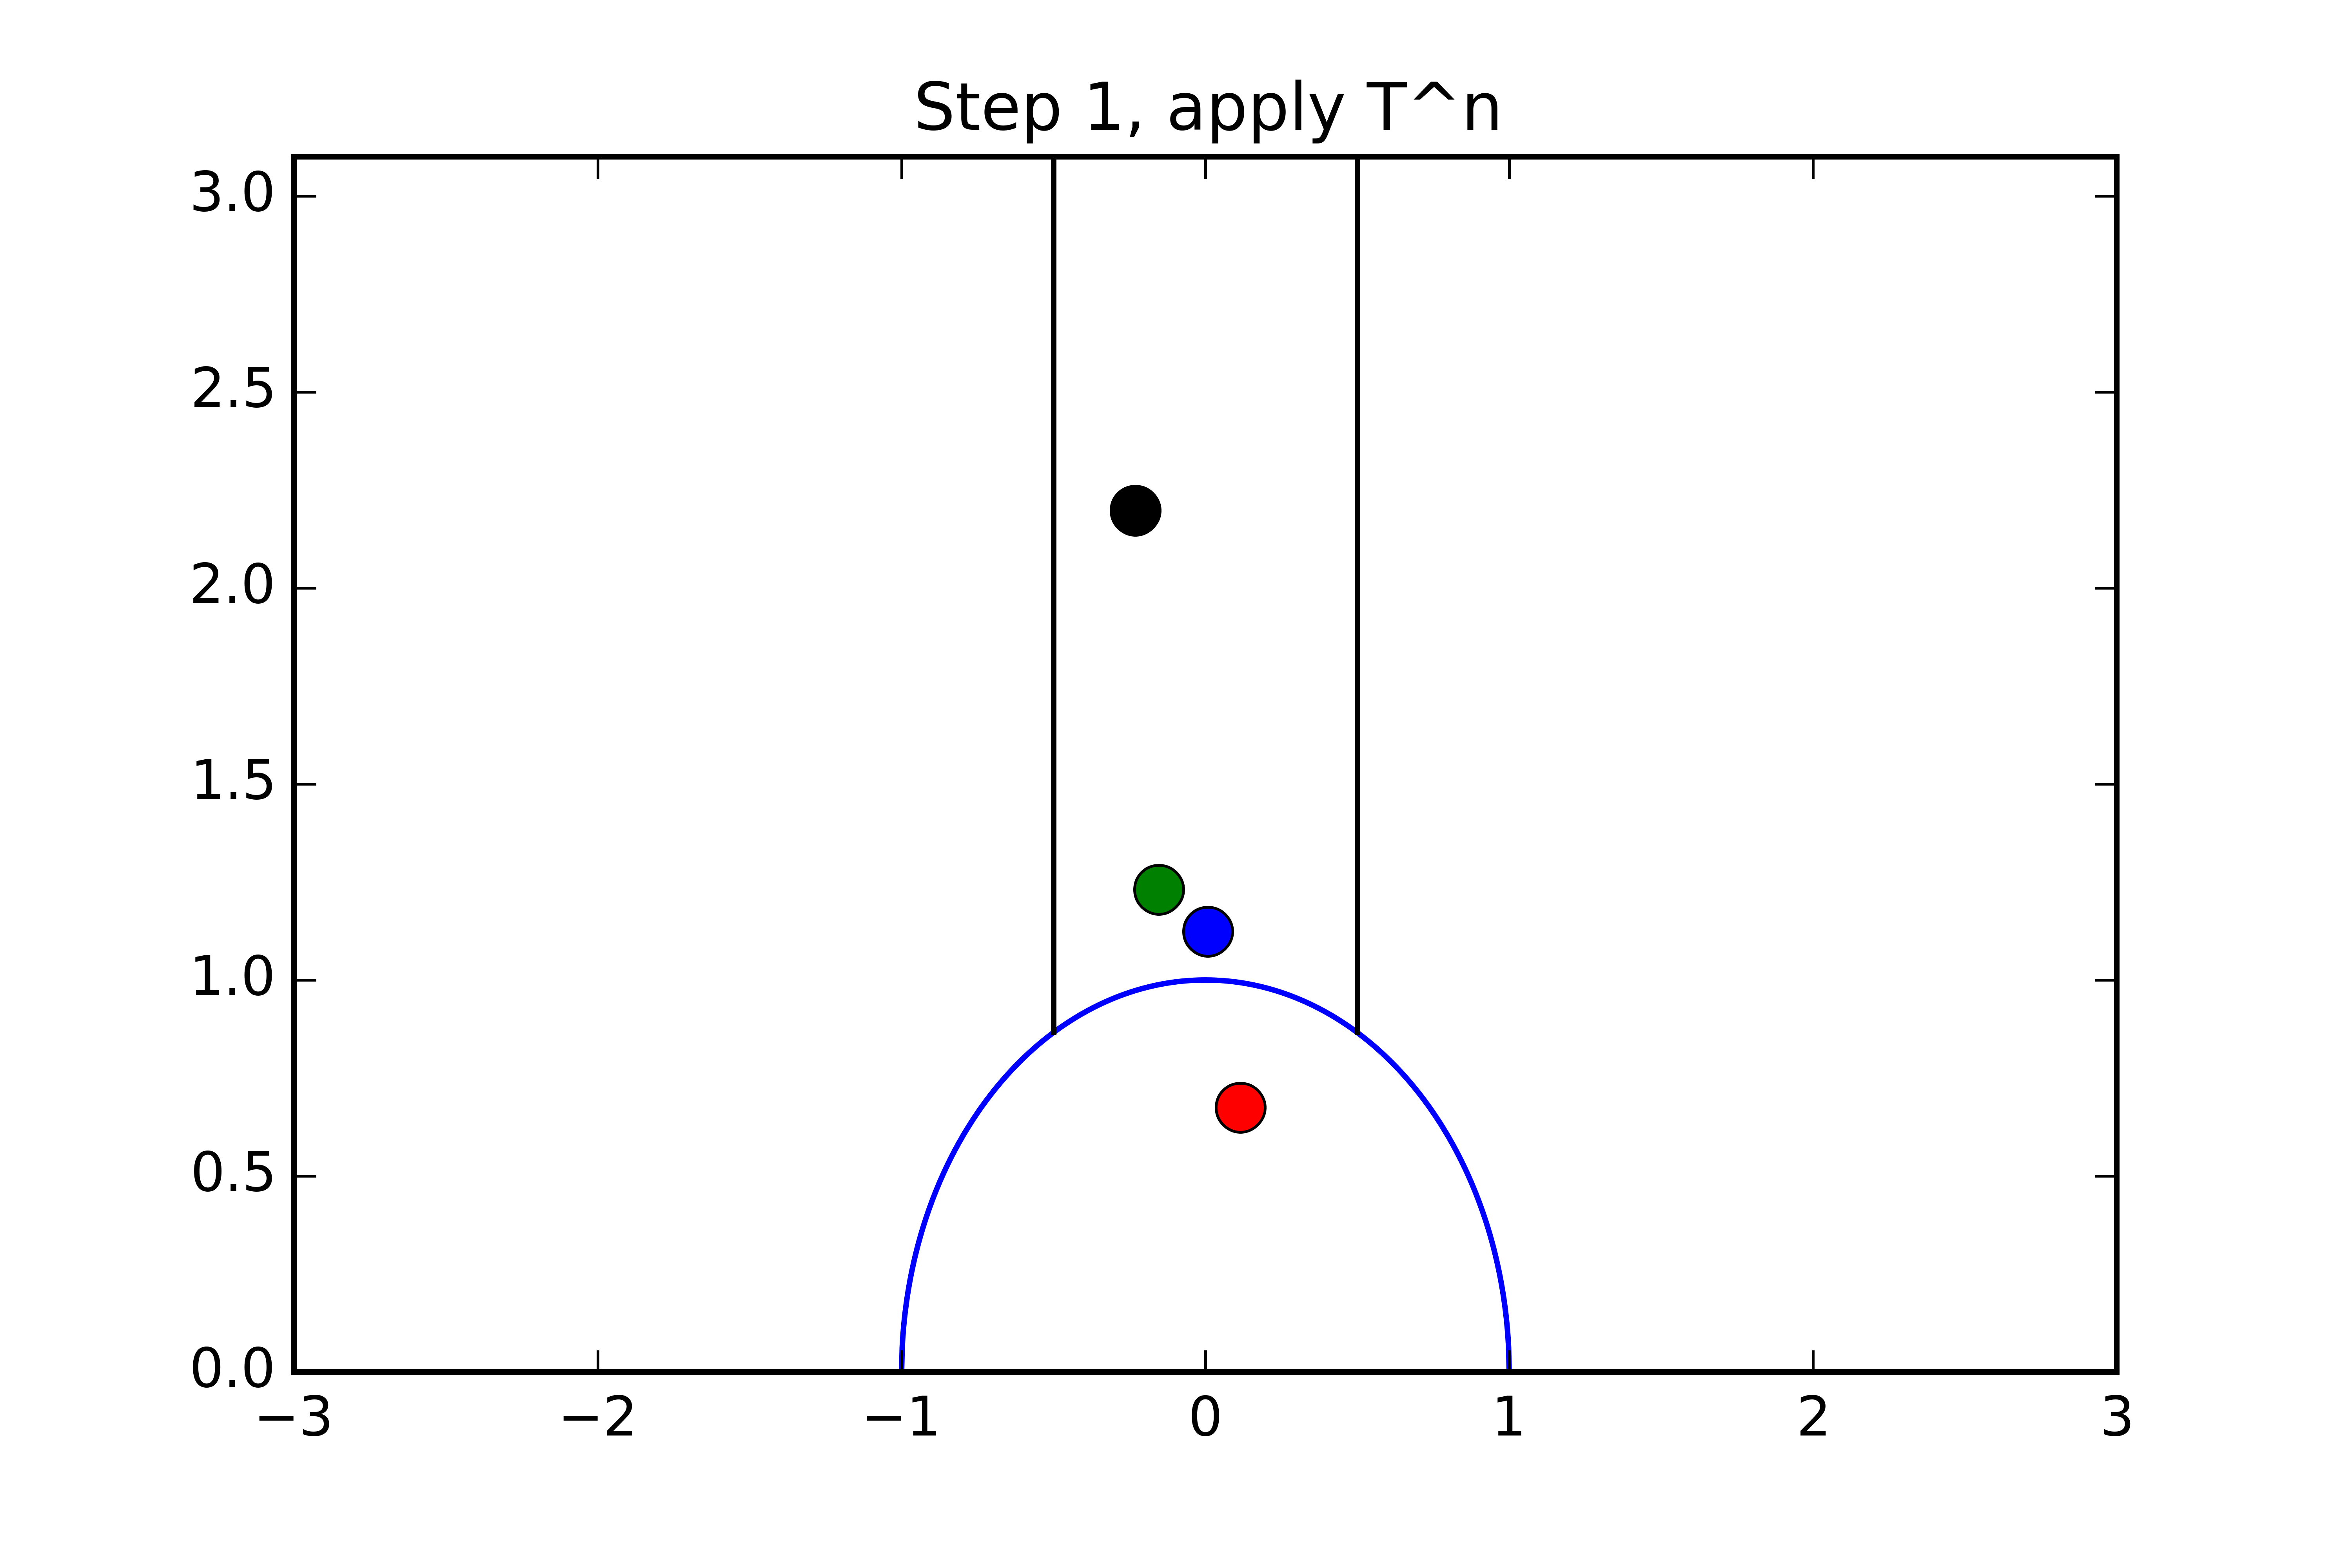
\includegraphics[width=65mm]{FundDomain-3} \\
(c) Apply S & (d) Apply $T^n$  \\[6pt]
\multicolumn{2}{c}{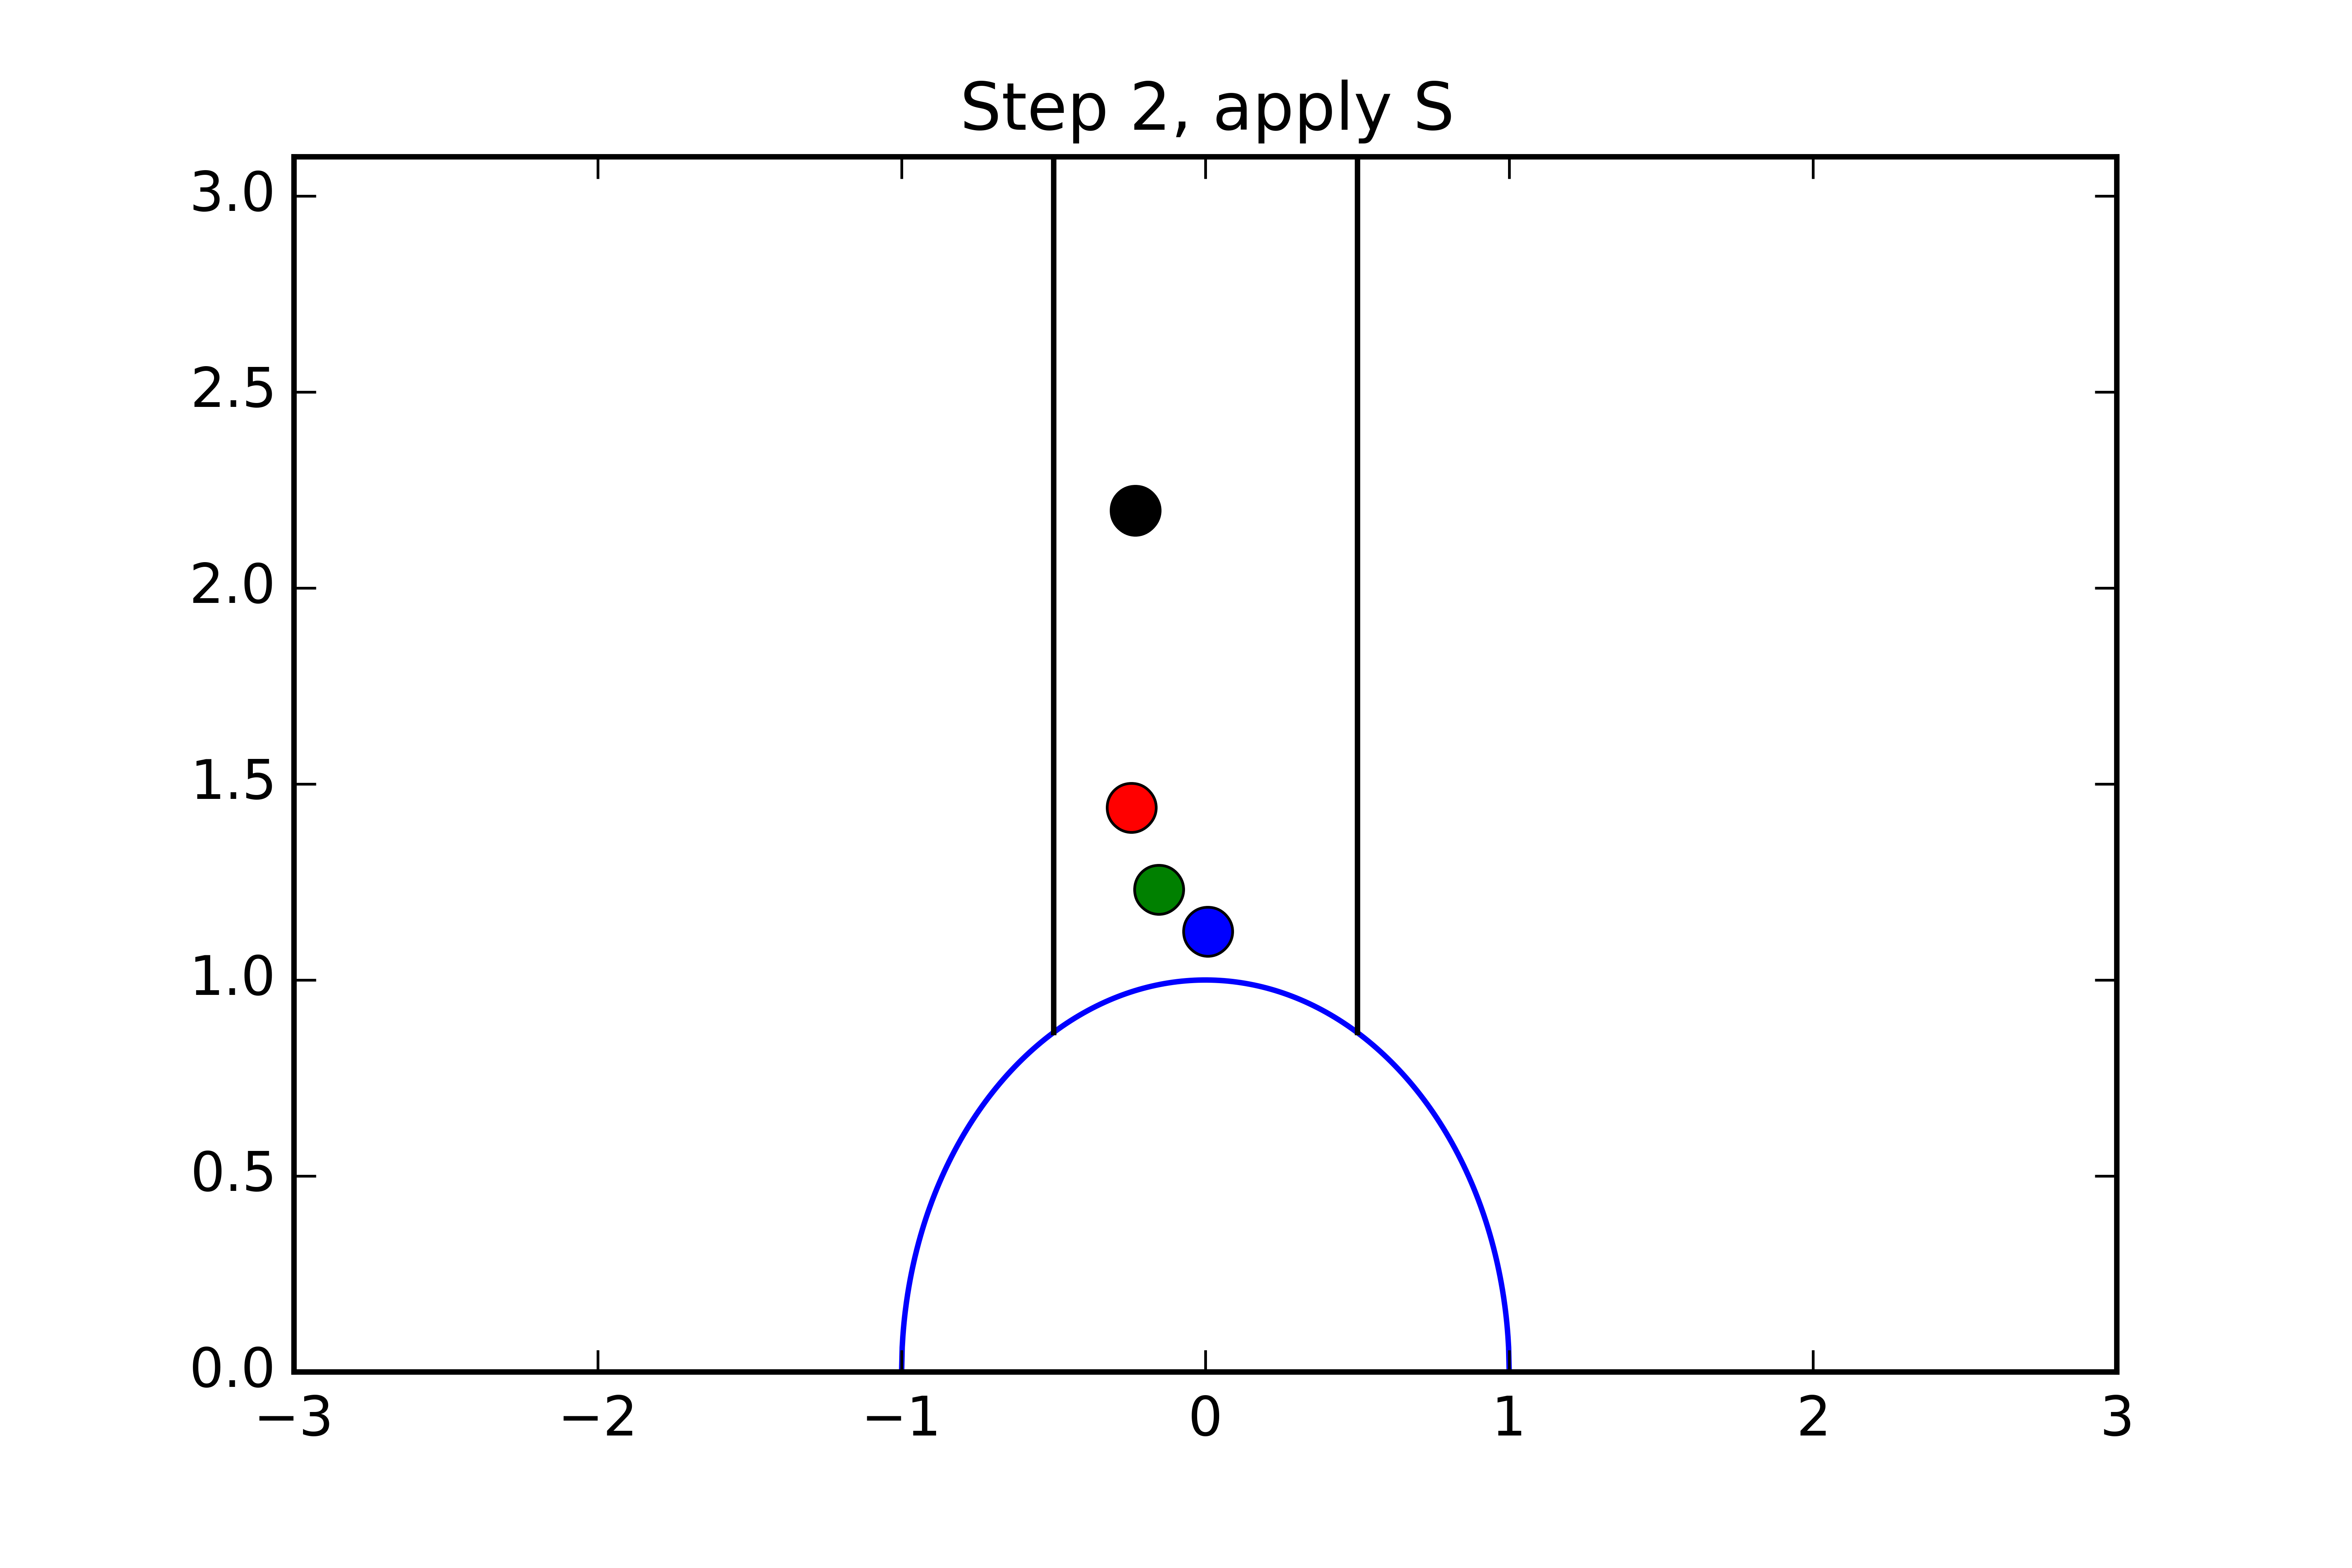
\includegraphics[width=65mm]{FundDomain-4} }\\
\multicolumn{2}{c}{(e) Apply $S$}
\end{tabular}
\caption{Example of procedure given in Lemma \ref{lem:gorbitfund} . }
\label{fig:procedure}

\end{figure}

\begin{lemma}\label{lem:noDistinctInteriorEquiv}
No two distinct points in the interior of $\mathcal{F}$ are $\Gamma$-equivalent
\end{lemma}

\begin{proof}

Suppose we have two distinct points $z_1, z_2 \in \mathcal{F}$ and there exists a $\gamma  = \abcd \in \Gamma$ such that $\gamma z_1 = z_2$. I.e $ -1/2 \leq Re(z_1), Re(z_2) \leq 1/2$ and $|z_1|, |z_2| \geq 1$.  We will show that both the points must lie on the boundary of $\mathcal{F}$. \\
Assume without loss of generality that $Im(z_1) \leq Im(z_2)$($\star$). \\
Writing out $Im(z_2)$ explicitly using \ref{eqn:imaginaryMobius}, 
\begin{align}
Im(z_2) = Im(\gamma z_1) &= \frac{Im(z_1)}{{|cz_1 +d |}^2} \overset{(\star)}{\geq} Im(z_1) \nonumber\\
& \implies |cz_1 + d | \leq 1 \label{eqn:boundCZD}
\end{align}
We will now investigate the possible values for $c,d$ based on the bound $|cz_1 +d | \leq 1$. The values we find for $c,d$ along with the condition on the determinant $ad -bc$ = 1 will allow us to determine all the possible matrices $\gamma$.\\
\\
If $|c| \geq 2$ then $Im(cz_1) \geq 2Im(z_1) \overset{Im(z_1) \geq 1}{\geq} \sqrt{3}$ and so $Im(cz_1 +d) > 1$. The imaginary part of $cz_1 +d$ thus lies outside the unit circle, it follows that the point $cz_1 +d$ lies outside the unit circle and so $|cz_1 +d| > 1$, which is a contradiction to \ref{eqn:boundCZD}. \\
The simplifies the possible $c,d$ pairs greatly since we must have $c \in  \{-1,0, 1\}$. \\
We consider the following cases separately, 
\begin{enumerate}[(i)]
\item $c = 0$: \\
Here the condition on the determinant means $ad = 1$ and so $a = d = \pm 1$. Thus $\gamma = \pm \left(\begin{array}{ c c } 1 & \pm b \\ 0 & 1 \end{array} \right)$, and so $\gamma = \pm T^{\pm b}$. \\
If $b = 0$ then $\gamma \pm I_2$ and so $\gamma z_1 = z_1$, which is a contradiction. \\
If $b \neq 0$, then $|Re(\gamma z_1)| = |Re(z_1) \pm b| \geq |Re(z_1) \pm 1| \geq  1/2$. So $\gamma z_1$ is only in $\mathcal{F}$ if $|Re(\gamma z_1)| = 1/2$, i.e only if $b = \pm 1$ and $\gamma = \pm T^{\pm 1}$. So $z_2 = z_1 \pm 1$, therefore they both lie on the boundary. 

\item $c = \pm 1$, $d = 0$: \\
The condition on the determinant gives $-bc = 1$ and so $c = -b = \pm 1$. Then $\gamma = \pm \left(\begin{array}{ c c } \pm a &  -1 \\ 1 & 0 \end{array} \right)$ thus it is of the form $\gamma = \pm T^{\pm a}S$. \\

The inequality \ref{eqn:boundCZD} gives $|\pm z_1 | = |z_1| \leq 1$, so $z_1$ since $z_1 \in \mathcal{F}$ we have $|z_1| = 1$. So $|Sz_1| = |-1/z_1| =1$. We are thus in the situation of (i) where we consider $-1/z_1$ instead of $z_1$, and $a$ in place of $b$. It follows that if $a = 0$, that $-1/z_1 = z_1$ and so $z_1^2 = -1$, the only solution in $\mathcal{H}$ is $z_1 = i$ and so $z_1= z_2$ and lies on the boundary of $\mathcal{H}$. \\
If $a \neq 0$ it follows from (i) that the only solution is $a = \pm 1$, and $-1/z_1 \pm 1 = z_1$. So the two possibilities are $z_1 = z_2 = \frac{1}{2} + i \frac{\sqrt{3}}{2}$ where $\gamma = \pm TS$ or $z_1 = z_2 = -\frac{1}{2} + i \frac{\sqrt{3}}{2}$ where $\gamma = \pm T^{-1}S$. These are the two points that lie both on the unit circle and one of the lines $Re(z)= \pm 1/2$. 

\item $c = \pm 1$, $d \neq 0$: \\
The inequality \ref{eqn:boundCZD} gives the condition $ |\pm z_1 +d | \leq 1$. But since $\mathcal{F}$ is symmetric this is equivalent to $|z_1 + d |\leq 1$. We can write it out fully as $|z_1 + d| = \sqrt{(x +d)^2 + y^2}$ where $z = x + iy$, firstly it's clear $|z_1 + d| \geq   \sqrt{(x +d)^2} = |(x +d)|$, since $y^2 > 0$. Suppose $|d| \geq 2$, then use $ -1/2 \leq x \leq 1/2$ to get $|x+d| \geq -1/2 +d$. Therefore $|\pm z_1 + d| \geq 3/2 > 1$ for $|d| \geq 2$, which is a contradiction. \\
So the only other possibility is $d = \pm 1$, We can repeat the above but include that the minimum value for $y$ is $\frac{\sqrt{3}}{2}$ and use the fact that $(x \pm 1)^2 \geq 1/4$ , so $|z_1 \pm 1| =\sqrt{(x \pm 1)^2 + y^2} \geq \sqrt{1/4 + 3/4} = 1$. Thus we must have 
$$|\pm z_1 \pm 1| = 1.$$
From this we go through all the possibilities: \\
Let $\omega^+ = \frac{1}{2} + i \frac{\sqrt{3}}{2}, \omega^- = -\frac{1}{2} + i \frac{\sqrt{3}}{2}$.
\begin{itemize}

\item Case, $c = d = 1$ : \\
Then $ |z_1 + 1| =1 \implies  z_1 = \omega^- $. The determinant of $\gamma$ is $a -b  =1 \implies a = b +1$. This means $\gamma =  \left(\begin{array}{ c c } b+1 &  b \\ 1 & 1 \end{array} \right)= T^{b+1}ST$, note $ST(z_1) = z_1$. \\
If $b = 0$, then $\gamma = \left(\begin{array}{ c c } 1 &  0 \\ 1 & 1 \end{array} \right) = TST$ and $\gamma z_1 =\omega^+$.\\
If $b = -1$ then $\gamma = \left(\begin{array}{ c c } 0 & -1 \\ 1 & 1 \end{array} \right) = ST$, $\gamma z_1 = z_1$.\\
For any other value of $b$ then $\gamma z_1$ will not lie in the fundamental domain.

\item Case, $c = -d = 1$ : \\
Then $|z_1 -1 | = 1 \implies z_1 = \omega^+$. The determinant of $\gamma$ is $ -a -b =1 \implies a = 1-b$. This means $\gamma =  \left(\begin{array}{ c c } 1-b &  b \\ 1 & -1 \end{array} \right) =  T^{-b}STS$, note $ STS(z_1) = \omega^-$. \\
If $b = 0$, then $\gamma = \left(\begin{array}{ c c } -1 &  0 \\ 1 & -1 \end{array} \right) = STS$ and $\gamma z_1 = \omega^-$.\\
If $b =-1$, then $\gamma = \left(\begin{array}{ c c } 0 &  -1 \\ 1 & 1 \end{array} \right) = (TS)^2$, and $\gamma z_1 = z_1$.\\
For any other value of $b$ then $\gamma z_1$ will not lie in the fundamental domain.

\item Case, $c = d = -1$ : \\
Then $|-z_1 - 1| = |z_1 +1| = 1  \implies z_1 = \omega^-$. The determinant of $\gamma$ is $-a + b =1 \implies a = b-1$. This means $\gamma =  \left(\begin{array}{ c c } b-1 &  b \\ -1 & -1 \end{array} \right) = -T^{-b}TST$, note $TST(z_1) = \omega^+$. \\
If $b = 0$, then $\gamma = \left(\begin{array}{ c c } -1 &  0 \\ -1 & -1 \end{array} \right) = -TST$, and $\gamma z_1 = \omega^+$. \\
If $b = 1$, the n $\gamma =  \left(\begin{array}{ c c } 0 &  1 \\ -1 & -1 \end{array} \right) = -ST$, and $\gamma z_1 = z_1$.

\item Case, $c = -d = -1$ : \\
Then $|-z_1 + 1| =1 \implies z_1 = \omega^+$. The determinant of $\gamma$ is $a +b =1 \implies a = 1-b$. This means $\gamma =  \left(\begin{array}{ c c } 1-b &  b \\ -1 & 1 \end{array} \right) = -T^{b}STS$, note $ STS(z_1) = \omega^-$. \\
If $ b = 0$, then $\gamma = \left(\begin{array}{ c c } 1 &  0 \\ -1 & 1 \end{array} \right) = STS$, and $\gamma z_1 = \omega^-$.\\
If $ b = 1$, then $\gamma = \left(\begin{array}{ c c } 0 &  1 \\ -1 & 1 \end{array} \right) = (TS)^2$, and $\gamma z_1 = z_1$

\end{itemize}

\end{enumerate}
\end{proof}

\begin{proposition}\label{prop:fundamentalDomain}
$\mathcal{F} = \{z \in \mathcal{H} \, | \, -1/2 \leq z \leq 1/2 \, |z| \geq 1  \}$ is a fundamental domain for $\Gamma$.
\end{proposition}
\begin{proof}
By applying Lemmas \ref{lem:gorbitfund} and \ref{lem:noDistinctInteriorEquiv} we see that $\mathcal{F}$ satisfies both parts of the definition for a fundamental domain. 
\end{proof}

\begin{figure}[!htbp]
  \begin{center}
    \leavevmode
    \ifpdf
      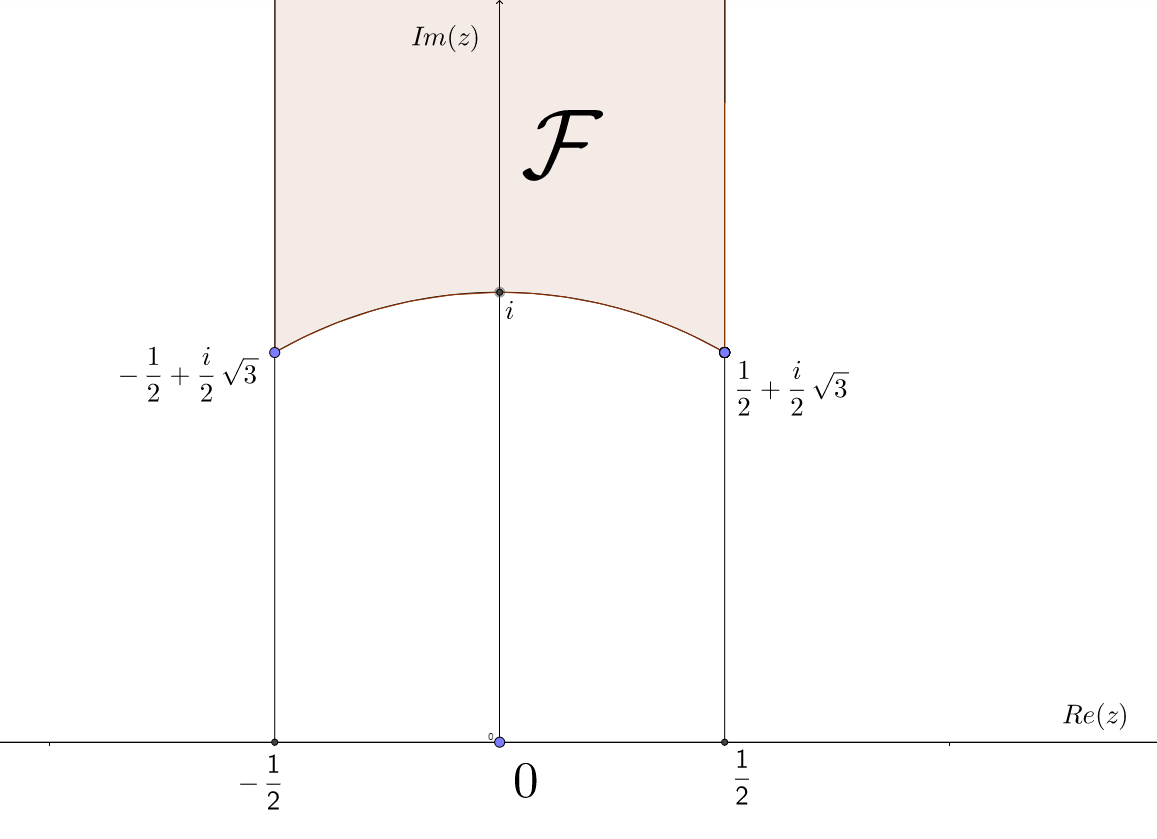
\includegraphics[height=3in]{FundamentalDomainGamma}
    \else
      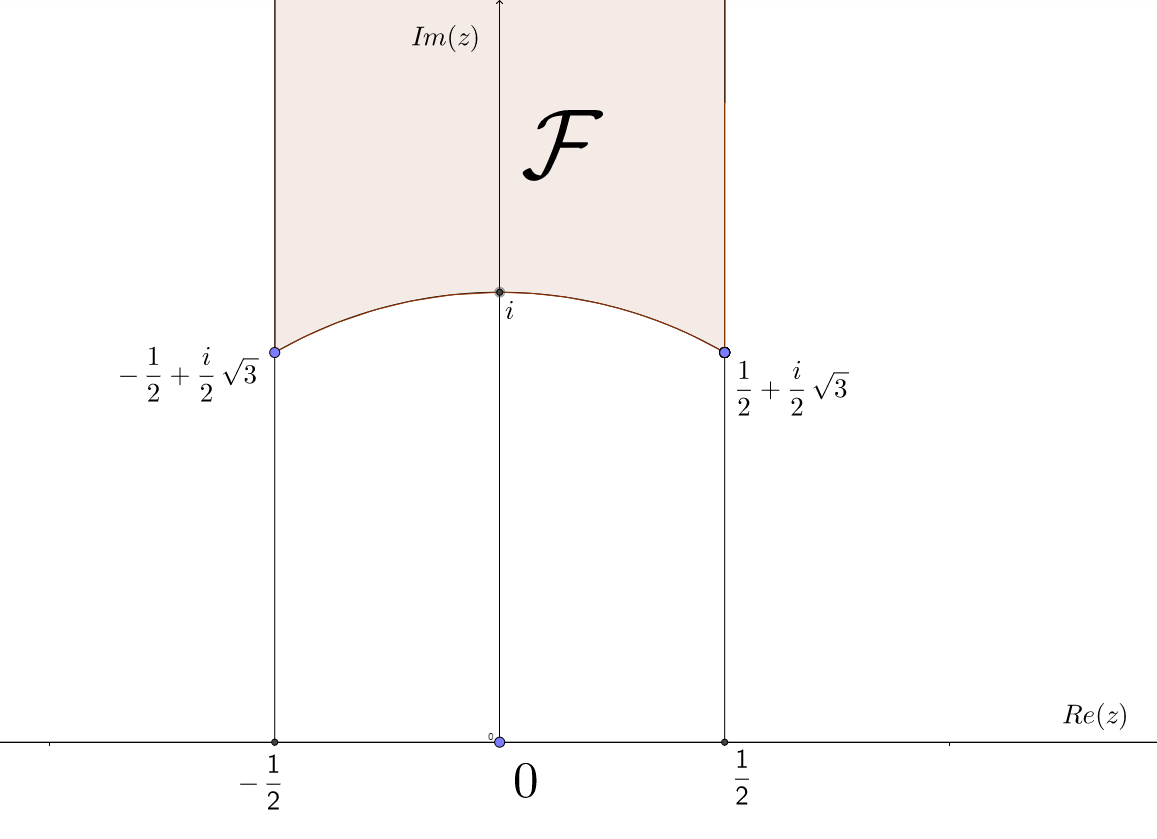
\includegraphics[bb = 92 86 545 742, height=6in]{FundamentalDomainGamma}
    \fi
    \caption{A fundamental domain $\mathcal{F}$ of $\Gamma$}
    \label{fig:fundDomainGamma}
  \end{center}
\end{figure}


See \ref{fig:kleinTessellation} for a tessellation of $\mathcal{H}$ by Klein \citep{klein}.

\begin{figure}[!htbp]
  \begin{center}
    \leavevmode
    \ifpdf
      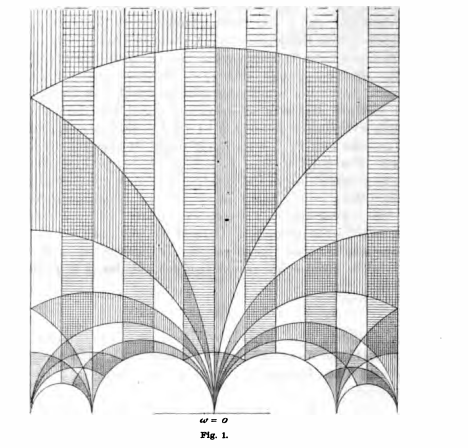
\includegraphics[height=3in]{KleinFundamentalDomain}
    \else
      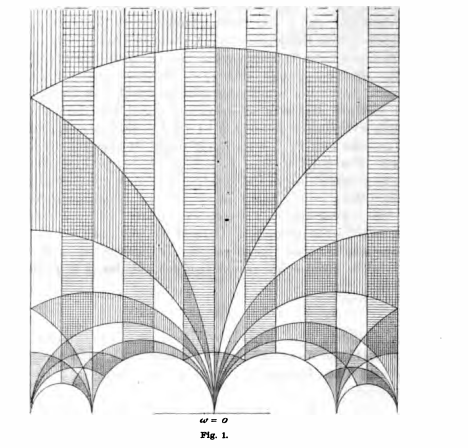
\includegraphics[bb = 92 86 545 742, height=6in]{KleinFundamentalDomain}
    \fi
    \caption{Tessellation of $\mathcal{H}$}
    \label{fig:kleinTessellation}
  \end{center}
\end{figure}


In the course of proving Lemma \ref{lem:noDistinctInteriorEquiv} we proved following two facts.
\begin{proposition}\label{prop:gammaEquivBoundary}
Two distinct points $z_1,z_2$ on the boundary of $\mathcal{F}$ are $\Gamma$-equivalent only if $Re(z_1) = \pm 1/2$ and $z_2 = z_1 \mp 1$ or $|z_1| =1$ and $z_2 = -1/{z_1}$
\end{proposition}

\begin{proposition}\label{prop:stabilizerGamma}
If $z \in \mathcal{F}$ then the stabilizer of $z$ in $\Gamma$, $\Gamma_z$, is $\{I,-I\}$, except in the following cases: \\
(i)   $\Gamma_z= \pm \{I,S\}$ if $z=i$\\
(ii)  $\Gamma_z= \pm \{I,ST, {(ST)}^2\}$ if $z=-1/2 + \frac{\sqrt{-3}}{2}$\\
(iii) $\Gamma_z= \pm \{I,TS, {(TS)}^2\}$ if $z=1/2 + \frac{\sqrt{-3}}{2}$\\
\end{proposition}


\begin{theorem}\label{thm:STGenerateSLTZGeometric}
The matrices $S,T$ generate $\Gamma$, i.e $\langle S, T \rangle =\sltz$.
\end{theorem}
\begin{proof}
Let $\gamma$ be an element of $\Gamma$, and let $z$ be a point in the interior of $\mathcal{F}$. Then consider the point $\gamma z \in \mathcal{H}$. In lemma \ref{lem:gorbitfund} we showed that there exists a $g \in \langle S, T \rangle$ such that $g \gamma z \in \mathcal{F}$. So the points $z$ and $g\gamma z$ are $\Gamma$ equivalent. 
But since $z$ is in the interior of $\mathcal{F}$ it follows from Propositions \ref{prop:fundamentalDomain} and \ref{prop:stabilizerGamma} that $g \gamma = \pm I_2$ and so $\gamma = g^{-1} \in \langle S, T \rangle$.
\end{proof}

The proof of Theorem \ref{thm:STGenerateSLTZGeometric} can be used to write an element $\gamma \in \Gamma$ as a word in $S, T$. Take a point in int($\mathcal{F}$), like $2i$, then consider the point $\gamma 2i$. We use the algorithm described the proof of Lemma \ref{lem:gorbitfund} to find $g \in \langle S, T \rangle$ such that $g \gamma 2i = 2i$ then $\gamma = g^{-1} \in \langle S, T \rangle$. 
\begin{example}
Consider the matrix $ \gamma = \left(\begin{array}{ c c }  1 & 1 \\ 1 & 2 \end{array} \right) \in \sltz$ and let $z = 2i \in \mathcal{F}$.
\\
Then $\gamma z = \frac{2i +1}{2i +2} = \frac{3}{4} + i\frac{1}{4}$.
\\
This lies outside the interval so we translate, $T^{-1}\gamma z = \frac{-1}{4} + i\frac{1}{4}$. However this is inside the unit circle so we invert to get $ST^{-1}\gamma z = 2 + 2i$. Again we do not lie in the interval so we need to translate. The translation by $T^2$ gives, 
$$T^{-2}ST^{-1}\gamma (2i) = 2i \text{ and so } \gamma = \left(\begin{array}{ c c }  1 & 1 \\ 1 & 2 \end{array} \right) = {(T^{-2}ST^{-1})}^{-1} = TST^2$$
\end{example}


\section{Algebraic approach to $\sltz$}

\subsection{Algebraic proof that $S,T$ generate $\sltz$ }
\label{subsect:proofAlgebraicSTGenerate}
It is possible to prove that $S, T$ generate $\sltz$ in a more direct way. We take a matrix in $\sltz$, and reduce it via the action of $S,T$ to the identity. Recall their action, 
$$S\abcd = \left(\begin{array}{ c c }  -c & -d \\ a & b \end{array} \right)\,,\quad 
T^n\abcd = \left(\begin{array}{ c c }  \pm a +cn & b+dn \\ c & d \end{array} \right).$$
Note also for any $n \in \mathbb{Z}$ that we can construct a matrix in $\sltz$ with lower left entry $n$, ex $A = \left(\begin{array}{ c c }  1 & 0 \\ n & 1 \end{array} \right) \in \sltz$.\\

\begin{proof}{(Algebraic)}\\
Let $A$ be a matrix in $\sltz$. \\
If $A$ has lower left entry 0, then it is of the form $ \left(\begin{array}{ c c } \pm 1 & m \\ 0 & \pm 1 \end{array} \right) = \pm T^m$ where $m \in \mathbb{Z}$. We know that $S^2 = -I_2$ so $A \in \langle S, T\rangle$. \\
We proceed by induction on the size of the lower left entry.
\\
The base case lower left entry equals 0 has been covered above.
\\
Let us assume that all matrices in $\sltz$ with lower left entry less in absolute value than $n+1$ are also in $\langle S, T\rangle$:
\\ 
Now suppose we have a matrix $A = \abcd$ with $\vert c \vert  = n +1$.\\
Case (i) : If $\vert a \vert < \vert c \vert$, then $SA  = \left(\begin{array}{ c c }  -c & -d \\ a & b \end{array} \right)$ has lower left entry $a$, with $\vert a \vert < n+1$ so by induction hypothesis $SA \in \langle S, T \rangle$ which implies $A \in \langle S, T \rangle$.\\
Case (ii) : If $\vert a \vert \geq \vert c \vert $, then use the division algorithm to write $a = cq + r$ where $ 0 \leq r < \vert c\vert$. Then 
$$T^{-q}A = T^n\abcd = \left(\begin{array}{ c c }  \pm a -cq & b-dq \\ c & d \end{array} \right) = T^n\abcd = \left(\begin{array}{ c c }  \pm r & b-dq \\ c & d \end{array} \right)$$.
$T^{-q}A$ has upper left entry $r$ where $\vert r \vert < \vert c \vert$, so we can use case (i) to conclude $T^{-q}A \in \langle S, T \rangle$ and so $A \in \langle S , T \rangle$.
\end{proof}

\begin{example}
We can carry out an example of the algebraic proof by hand. Let $A = \left(\begin{array}{ c c } 13 & 37 \\ 7 & 20 \end{array} \right)$. First observe $13 = 7\cdot 1 + 6$, so subtract the bottom row from the top, multiplying by $T^{-1}$,
$$T^{-1}A = \left(\begin{array}{ c c } 6 & 17 \\ 7 & 20 \end{array} \right).$$
Now $6>7$ so we interchange rows, multiplying by $S$, 
$$ST^{-1}A = \left(\begin{array}{ c c } 7 & 20 \\ -6 & -17  \end{array} \right).$$
And now we can write $7 = -6\cdot -1 +1$, so we add the second row to the first, with $T$
$$TST^{-1}A = \left(\begin{array}{ c c } 1 & 3 \\ -6 & -17  \end{array} \right).$$
We see that $|-6| > |1|$ so we invert with $S$,
$$STST^{-1}A = \left(\begin{array}{ c c } -6 & -17 \\ -1 & -3  \end{array} \right).$$
We can at last reduce the upper left entry to $0$, write $-6 = -1\cdot 6 + 0$, multiply by $T^{-6}$,
$$T^{-6}STST^{-1}A = \left(\begin{array}{ c c } 0 & 1 \\ -1 & -3  \end{array} \right).$$
And to switch this into correct from, swap rows using $S$ and get,
$$ST^{-6}STST^{-1}A = \left(\begin{array}{ c c } -1 & -3 \\ 0 & -1  \end{array} \right) = -T^3.$$
Rearrange this to get 
$$A = \left(\begin{array}{ c c } 13 & 37 \\ 7 & 20 \end{array} \right) = -TST^{-1}ST^6ST^3$$
While working through this example or reexamining the proof one might notice that this algorithm is not the only way to get a decomposition of $A$ in terms of $S,T$. For example in the first step we could multiply $A$ by $T^{-2}$ instead, and get,
$$T^{-2}A =  \left(\begin{array}{ c c } -1 & -3 \\ 7 & 20 \end{array} \right)$$
An advantage being we arrive at upper left entry with absolute value 1 in less steps, and so lower left entry 0 in less steps. Continuing the algorithm as normal from here we get the decomposition,
$$A =\left(\begin{array}{ c c } 13 & 37 \\ 7 & 20 \end{array} \right) = T^2ST^7ST^3$$
\end{example}

\begin{corollary}\label{cor:genFiniteOrderSST}
The group $\sltz$ is generated by two matrices of finite order. In particular $\sltz = \langle S, ST \rangle$
\end{corollary}
\begin{proof}
We have $\sltz = \langle S, T \rangle$. So $\langle S, ST \rangle \subset \sltz$. But also $S \in \langle S, ST \rangle$ and $T = S^3(ST) \in \langle S, ST\rangle$. So $ \sltz = \langle S, T \rangle =  \langle S, ST\rangle$. The matrix $S = \sm$ has order 4 and $ST = \left(\begin{array}{ c c } 0 & -1 \\ 1 & 1 \end{array} \right)$ has order 4.
\end{proof}

\begin{corollary}\label{cor:genInfiniteOrderUT}
The group $\sltz$ is generated by two matrices of infinite order. In particular $\sltz = \langle T, U \rangle $, where $T = \tm$ and $U = \left(\begin{array}{ c c } 1 & 0 \\ 1 & 1 \end{array} \right)$.
\end{corollary}
\begin{proof}
Both $T$ and $U$ are in $\sltz$, so $\langle T, U \rangle \subset \sltz$. Conversely, since $S = T^{-1}UT^{-1}$, $\langle T, U \rangle \supset \langle S, T \rangle = \sltz$.
\end{proof}
\numberwithin{equation}{section}

\externaldocument{chapter1}

\chapter{Congruence subgroups of $\sltz$}

\section{The principal congruence subgroup $\Gamma(N)$}
Recall the notation $\sltz = \Gamma$. 
\begin{definition} The group denoted $\Gamma(N)$,  $N \in \mathbb{N^+}$, is called the principal congruence subgroup of level $N$, defined to be
$$\Gamma(N) := \Big  \lbrace  A= \left(\begin{array}{ c c } a & b \\ c & d \end{array} \right) \in \Gamma \, \Big \vert \, A \equiv   \left(\begin{array}{ c c } 1 & 0 \\ 0 & 1 \end{array} \right) \mod N \Big  \rbrace$$
We define $\Gamma(1)  := \Gamma$.
\end{definition}
This subgroup $\Gamma(N)$ is actually a normal subgroup in $\Gamma$ since it is the kernel of the group homomorphism from $\sltz \rightarrow \sltznz$ obtained by reducing entries modulo $N$. Notice that $a \equiv x \mod Nt \implies a \equiv x \mod N$ so for any multiple $Nt$ we get $\Gamma(Nt) \subset \Gamma(N)$.
\\
We will make use of the following elementary lemma in several proofs.
\begin{lemma}\label{lem:elementaryCoprime}
Given integers $c \neq 0,\, d,\, N  \in \mathbb{Z}$. The set $\{t \, \vert \, (d + tN, c) = 1 \}$ is non-empty, and this set is infinite if there exists a prime dividing $c$ but not $d$. (I.e $\gcd(c,d) \neq c \text{ or }  d$).
\end{lemma}
\begin{proof}
Let $d' = d+ tN$. Our goal is to find appropriate values for $t$.
\\ 
We begin by splitting the prime divisors of $c$ into two groups, 
\\ 
$$\{p_1,p_2,\dots,p_s \colon \, p_i \mid c \,,\, p_i \mid d\} \text{ and } \{q_1,q_2,\dots, q_r \colon q_j \mid c\, ,\, q_j \nmid d\}$$

If $\gcd(c,d) \neq c \text{ or } d$ : then the set of $q_j$ is non empty.\\
Define $k = \prod{q_j} = \prod_{p\mid c,p\nmid d}p$, and $d' = d + tN$, where $t = k^m$. Where $m$ any positive integer.\\
Suppose $p$ is a prime divisor of $c$ and $d'$. \\
Suppose also $p \mid d$, then $p \mid (d' -d)  = tN$ and $p \nmid t$. This implies $p \mid N$, which is a contradiction, since $\gcd(c,dN) =1$. \\
Otherwise if $p \nmid d$, then $p \nmid (d' -d) = tN$ and $p \mid t$. These two results contradict.  \\
So there are no common prime divisors of $c,d'$ and so $gcd(c,d' = d + k^m) = 1$, for all $m \in \mathbb{N}$.\\
\\
In the other case, if $\gcd(c,d) = c \text{ or } d$, define $d' = d+ N$. Now $\gcd(c,d') =1$ since $\gcd(c,d,N) =1$.
\end{proof}

\begin{theorem}\label{thm:surjective}
The natural map $\sltz \rightarrow \sltznz$ is surjective.
\end{theorem}

\begin{proof}
Let $\gamma = \left( \begin{array}{ c c } \bar{a} & \bar{b}  \\ \bar{c} & \bar{d} \end{array} \right) \in \sltznz$ be given. A lift of $A \in \sltznz$ to  $M_2(\mathbb{Z})$ is an element in the inverse image of $A$ by the reduction homomorphism. Let $\tilde{\gamma} = \left(
  \begin{array}{ c c }
     a & b \\
     c & d
  \end{array} \right) \in M_2(\mathbb{Z})$, such that $\tilde{\gamma} \equiv \gamma \mod N$.
We show it's possible to modify $\tilde{\gamma}$ such that it's still congruent to $\gamma$ but has unit determinant.\\
\\
First note that $ad -bc \equiv 1 \mod N$. So $ad - bc +Nk = 1$ for some $k \in \mathbb{Z}$, so $\gcd(c,d,N) = 1$.\\
We suppose $c \neq 0$ for now. We can apply Lemma \ref{lem:elementaryCoprime} to find a $d'$ such that $\gcd(c,d') =1$, and $d' \equiv d \mod N$. Define $\tilde{\gamma_1} = \left( \begin{array}{ c c } a & b \\ c & d' \end{array} \right) \equiv \gamma$.\\
We can now consider lifts of $\gamma$ of form $ \tilde{\gamma_2} = \left(
    \begin{array}{cc}
        a+kN & b+lN  \\
        c    & d'
    \end{array} \right)$, $k,l \in \mathbb{Z}$. The determinant is $\det(\tilde{\gamma_2}) = (a+kN)d' - (b+lN)c = ad' - bc +N(kd'-lc)$.\\  From the definition of $\gamma_1$ we have $ad' - bc = 1 + qN$ for some $q\in \mathbb{Z}$. By substitution, $\det(\tilde{\gamma_2}) = 1 + N(q + kd' - lc) = 1$.\\
Now the fact that $\gcd(c,d') = 1$ allows us to solve $q = lc - kd'$ for $k,l 
\in \mathbb{Z}$. We obtain the lift,
$$\left(
    \begin{array}{cc}
        a +kN & b +lN  \\
        c    & d'
    \end{array} \right) \in \sltz \equiv \gamma \mod N$$
The case $c = 0$ is not much different. The condition $\det(\gamma) =1$ gives that $d \neq 0$, and we proceed similarly to above. We have $\gcd(a,d,N) =1$, and we set $d' = d + tN$ where $t = \prod_{p\mid a,p\nmid d}p$. This gives $gcd(d',a) =1$. Then we compute $q$ from $ad = 1+qN$. Finally we solve $ax + yd' = -q$ for integers $x, \,y$. Our desired lift is then $\left(
    \begin{array}{cc}
        a+yN & b  \\
        0    & d' + xN
    \end{array} \right)$
\end{proof}


\begin{theorem} \label{thm:-IT2U2genGamma2}
The group $\Gamma(2)$ is generated by the matrices $-I,T^2$ and $U^2$, where $T = \tm,U = \um$ as before, so $T^2 = \left(\begin{array}{ c c } 1 & 2 \\ 0 & 1 \end{array} \right)$ and $U^2 = \left(\begin{array}{ c c } 1 & 0 \\ 2 & 1 \end{array} \right)$. 
\end{theorem}
\begin{proof}
We have that $-I,T^2,U^2 \in \Gamma(2)$  so $\langle -I,T^2,U^2 \rangle \subset \Gamma(2)$. For the reverse inclusion we adapt the algebraic proof that $\langle S,T\rangle = \sltz$. We will use the modified division theorem, that is, given $a,b \in \mathbb{Z}$ we can write $a = bq + r$ where $ |r| \leq |b|/2$.\\
So we pick any $A  =  \left(\begin{array}{ c c } a & b \\ c & d \end{array} \right) \in \Gamma(2)$, the definition gives that $a,d$ are odd and $b,c$ are even. \\
If $c=0$, then $ad-bc = ad = 1$ implies that $a=d = \pm 1$, also $b$ is even so can write as $b = 2k$ so $A =  \left(\begin{array}{ c c } \pm 1 & 2k \\ 0 & \pm 1 \end{array} \right) \in \Gamma(2)$. This is of the form $ \pm T^{2k} = \pm {T^2}^k \in \langle -I, T^2 \rangle$.\\
What we wish to show is that every matrix in $\Gamma(2)$ can be reduced to a matrix with lower left entry 0 by an element of $-I,T^2,U^2$.
We can proceed by induction on the size of $c$, the lower left entry. If $c=0$ we are done by the above.\\
Suppose every matrix in $\Gamma(2)$ with lower left entry,$c$ , such that $|c| < n$, can be reduced to a matrix with lower left entry 0 by an element of $-I,T^2,U^2$. \\
Now suppose we have a matrix $\left(\begin{array}{ c c } a & b \\ c & d \end{array} \right) \in \Gamma(2) $ with $ |c| = n$. From the definition of $\Gamma(2)$ we see that $a$ and $c$ have different parity, so $|a| \neq |c|$, there are two possibilities.
If $|a| < |c|$, use the modified division theorem to write $c = (2a)q + r$, where $|r| \leq |2a|/2 =|a|$. Then 
$$U^{-2q}A =  \left(\begin{array}{ c c } 1 & 0 \\ -2 & 1 \end{array} \right)\left(\begin{array}{ c c } a & b \\ c & d \end{array} \right) = \left(\begin{array}{ c c } a & b \\ c-2qa & d-2qb \end{array} \right) = \left(\begin{array}{ c c } a & b \\ r & d-2qb \end{array} \right)$$.
Now the matrix $U^{-2q}A$ has lower left entry $r$, and $|r| < |c|$, i.e lower left entry less in absolute value than before, so we can conclude by the induction hypothesis.
If $|a| > |c|$, then use the modified division theorem to write $a = (2c)q + r$, where $|r| \leq |2c|/2 = |c|$. Then 
$$T^{-2q}A = \left(\begin{array}{ c c } 1 & -2 \\ 0 & 1 \end{array} \right)\left(\begin{array}{ c c } a & b \\ c & d \end{array} \right) =  \left(\begin{array}{ c c } a-2qc & b-2qd \\ c & d \end{array} \right) = \left(\begin{array}{ c c } r & b-2qd \\ c & d \end{array} \right)$$ 
Now the upper left entry $r$ is less in absolute value than the lower left entry so we can apply the first case and then conclude by induction.
\\
This shows we can find $g \in  \langle -I, T^2, U^2 \rangle$, such that $gA$ has lower left entry 0. This is of the form $gA = \pm T^{2k} \in \langle -I, T^2 \rangle \implies A = \pm g^{-1} T^{2k} \in \langle -I, T^2, U^2 \rangle$.

\end{proof}




\begin{lemma}\label{lem:orderofslznzpe}
The order of $\sltznz[p^e] $ is $p^{3e}( 1- 1/p^2)$ when $p$ is prime and $e \in \mathbb{N}$. 
\end{lemma}
\begin{proof}
 The case $e=1$ can be computed by considering two subcases and counting the number of possible $A =  \left(\begin{array}{ c c }  a& b \\ c & d \end{array} \right) \in \sltznz[p] $. The definition of $\sltznz[p]  $ gives us that $A \in \sltznz[p]  $ if and only if $ det(A) = ad -bc \equiv 1 \mod p$. The number of solutions to this equation in $\mathbb{Z}/p\mathbb{Z}$ is equal to the number of possible $A$. A key fact we will use is that $(\mathbb{Z}/p\mathbb{Z})^* = \znz[p] \setminus \{\bar{0}\}$, so each non-zero element in $\znz$ has a unique multiplicative inverse ($\star$).\\
 
    Case $a\equiv0$ : $A =  \left(\begin{array}{ c c }  0 & b \\ c & d \end{array} \right)$, and $\det(A) = -bc \equiv 1\mod p$. We can apply $(\star)$ to say there are $p-1$ solutions in $b,c$ to this congruence. Also $d$ can take any of $p$ values in $\znz$. The total gives $p\cdot(p-1) = p(p-1)$ solutions to $ad -bc \equiv 1 \mod p$ for $a \equiv 0,b,c,d  \in \znz[p]$. \\
    
    Case $a\not \equiv 0$ : We can rearrange the equation to $ad \equiv 1+bc \mod p$. There are $p-1$ possible values for $a \not \equiv 0$, and $p$ possible values for each $b$ and $c$. From these the value for $d$ is determined uniquely by $(\star)$. In total there are $(p-1)\cdot p \cdot p \cdot 1 = (p-1)p^2$ in solutions to $ad -bc \equiv 1 \mod p$ for $a \not \equiv 0, b,c,d \in \znz[p]$.
\\    
    Totaling from both cases we have $p(p-1) + (p-1)p^2 = p^3 - p$ solutions to the equation for determinant. So the order of $\sltznz[p]$  is $p^3 - p$.\\
    The case  $e>1$ is more complex since then for $a\not\equiv 0$ the relation $ad \equiv 1+bc \mod p^e$ is not always solvable so we would have to separately consider further subcases $a$ invertible and not invertible $\mod p$. \\ 
We can proceed by induction on $e$.  We have shown $\sltznz[p^e] \vert = p^{3e}(1 - 1/p^2)$ for $e =1$. \\
Suppose that the result holds for $e = k$, i.e
$$\vert \sltznz[p^k] \vert = p^{3k}(1 - 1/p^2).$$ 
Consider the reduction homomorphism 
$$f: \sltznz[p^{k+1}] \to \sltznz[p^k] $$
$$f(\left(\begin{array}{ c c }  a& b \\ c & d \end{array} \right) = \left(\begin{array}{ c c }  a & b \\ c & d \end{array} \right) \mod p^k$$
The kernel of $f$ is, $$\Big \lbrace A \in \sltznz[p^{k+1}]  \Big \vert A = \left(
      \begin{array}{ c c }
         1+a'p^k & b'p^k \\
         c'p^k &  1+d'p^k 
      \end{array} \right) \text{ and } 0 \leq a',b',c',d' < p \in \mathbb{Z}/p^{k+1}\mathbb{Z} \Big \rbrace $$
Again we can count the number of possible matrices by counting the number of solutions to the determinant equation.
\begin{align*}
A\in ker(f) &\iff \det(A) \equiv 1 \mod p^{k+1}\\
			 & \iff  ( 1+a'p^k)( 1+d'p^k ) - (b'p^k)(c'p^k) \equiv 1 \mod p^{k+1}\\
             & \iff  1 + a'p^k + d'p^k + a'd'p^{2k} - b'c'p^k \equiv 1 \mod p^{k+1}\\
             & \iff   a'p^k + d'p^k  \equiv 0\mod p^{k+1}\\
             & \iff a' \equiv -d' \mod p
\end{align*}
So we if we let $d' = np -a'$ for some $n \in \znz[p]$, we can rewrite,
\begin{align*}
\lbrace A \in \sltznz[p^{k+1}]  \Big \vert A = \left(
      \begin{array}{ c c }
         1+a'p^k & b'p^k \\
         c'p^k &  1+(np- a')p^k 
      \end{array} \right) \\
       \text{ and } 0 \leq a',b',c', (np -a') < p\,, n\, \in \mathbb{Z}/p^{k+1}\mathbb{Z} \Big \rbrace
\end{align*}  
The restriction $0\leq a',(np - a') < p$ means we must have $n =1$. A matrix in $ker(f)$ is thus determined uniquely by the values $0 \leq a',b',c' < p$. The order of $ker(f)$ is thus the product of the number of possibilities for each value, ie $ker(f) = p^3$.\\ 
The reduction map $f$ is also surjective, this is because the reduction map from $\sltz \rightarrow \sltznz[p^k] $ is surjective and it can be decomposed into two maps $\sltz \rightarrow \sltznz[p^{k+1}]   \overset{f}{\rightarrow} \sltznz[p^k] $, so both the intermediate maps must be surjective.\\ 
We can apply the first isomorphism theorem to obtain $\sltznz[p^{k+1}] /ker(f) \cong \sltznz[p^k] $, and so
$$\vert \sltznz[p^{k+1}] \vert  = p^3 \vert \sltznz[p^k] \vert  \stackrel{\text{induction}}{=} p^{3(k+1)}(1 - 1/p^2)$$
\end{proof}

\begin{proposition} \label{prop:chineseRemainderTheorem}
Let $N\in \mathbb{Z}$, then, 
$$ \sltznz \cong \prod_{i=1}^k \sltznz[p_{i}^{r_i}]$$
Where $N = p_{1}^{r_1}\cdot\dots\cdot p_{k}^{r_k}$ is the prime factorization.
\end{proposition}
\begin{proof}
If we write $N$ as it's prime factorization $N = p_{1}^{r_1}
    \cdot\dots\cdot p_{k}^{r_k}$.
Define the homomorphism,
    $$f \, : \, \sltznz \to \prod_{i=1}^k \sltznz[p_{i}^{r_i}]$$
    $$\left(
      \begin{array}{ c c }
         a & b \\
         c & d
      \end{array} \right) \mapsto \Big( \left(
      \begin{array}{ c c }
         a & b \\
         c & d
      \end{array} \right) \mod p_{1}^{r_1} ,\dots, \left( \begin{array}{ c c }
         a & b \\
         c & d
      \end{array} \right) \mod p_{k}^{r_k} \Big)$$
      The function $f$ is well-defined, let $x\in \mathbb{Z}$, 
\begin{eqnarray*}
x \equiv x' \mod N \iff  N \mid (x-x') & \iff  & p_{1}^{r_1} \dots p_{k}^{r_k} \mid (x-x') \\
& \implies & p_i^{r_i} \mid (x-x') \iff x \equiv x' \mod  p_i^{r_i}
\end{eqnarray*}
\\
      To show $f$ is surjective, suppose we have  $\Big( \left(
      \begin{array}{ c c }
         a_1 & b_1 \\
         c_1 & d_1
      \end{array} \right) \in \sltznz[p_{1}^{r_1}],\dots, \left( \begin{array}{ c c }
         a_k & b_k \\
         c_k & d_k
      \end{array} \right) \in \sltznz[p_{k}^{r_k}]  \Big)$ 
      then we can find a matrix $A = \abcd \in M_2(\znz)$ by solving the corresponding system of congruences for each entry using the Chinese Remainder Theorem. For example, we take $a$ as the solution to the system \big($a \equiv a_1 \mod p_1^{r_1}\, ,\dots,a \equiv a_k \mod p_k^{r_k}$\big). We also must check $A$ does indeed lie in $\sltznz$, i.e $\det(A) \equiv 1 \mod N$. 
\\ 
For each $\left(\begin{array}{ c c }
         a_i & b_i \\
         c_i & d_i
      \end{array} \right) \in \sltznz[p_{i}^{r_i}]$ we have $a_i d_i - b_i c_i \equiv 1 \mod p_{i}^{r_i}$. Then $ad -bc \equiv 1 \mod p_{i}^{r_i}$ by definition of $a,b,c,d$. From this we see $p_{i}^{r_i} \mid (ad -bc ) -1$ for each prime power $p_{i}^{r_i}$, it follows that $ N = \prod_{i=1}^k p_{i}^{r_i} \mid (ad -bc) -1$. So $ ad -bc \equiv 1 \mod N$ and $A \in \sltz$.
\\
      To show injectivity suppose,
      $$f\big( \left(
      \begin{array}{ c c }
         a & b \\
         c & d
      \end{array} \right) \big) = f\big( \left(
      \begin{array}{ c c }
         a' & b' \\
         c' & d'
      \end{array} \right) \big)$$
      Then $a \equiv a' \mod p_i^{r_i}$ so by the Chinese Remainder Theorem $a \equiv a' \mod  p_{1}^{r_1} \dots p_{k}^{r_k} = N$, similarly we get $b\equiv b' \mod $, $c\equiv c' \mod N$,$d\equiv d' \mod N$.
\end{proof}


\begin{corollary} \label{cor:ordersltznz}
The order of $\sltznz$ is $N^3\prod_{p \mid N}(1 - 1/p^2)$.
\end{corollary}

\begin{proof}
From Proposition \ref{prop:chineseRemainderTheorem} we have $ \sltznz \cong \prod_{i=1}^k \sltznz[p_{i}^{r_i}]$.
So $$\vert \sltznz \vert = \prod_{p^e \mid N}\vert \sltznz[p^e]\vert = \prod_{p^e \mid N}p^{3e}(1 - 1/p^2)  = N^3\prod_{p \mid N}(1 - 1/p^2) $$
\end{proof}


\begin{corollary}\label{cor:generateordern}
The finite group $\sltznz$ is generated by two elements of order $N$. 
\end{corollary}

\begin{proof}
Every element of $\sltznz$ has a lift in $\sltz$. In Corollary \ref{cor:genInfiniteOrderUT} we showed $\langle T, U \rangle = \sltz$, where $T = \left(\begin{array}{ c c }  0& 1 \\ 1 & 1 \end{array} \right)\,,\, U = \left(\begin{array}{ c c }  1& 1 \\ 0 & 1 \end{array} \right)$. So this lift can be written as an element of $\langle T, U \rangle$. So reducing the lift modulo $N$ we get it as a product $T,U$ modulo $N$, i.e 
$$\sltznz = \langle \, T \mod N, U \mod N \, \rangle.$$ 
Also $T^n = \tm[n], U^n = \um[n]$ for all $n \in \mathbb{Z}$, so both have order $N$.
\end{proof}


\begin{corollary}\label{cor:reductionIsomorphism}
For any integer $N > 1$, 
$$\sltznz \cong \sltz / \Gamma(N) \text{ and } [\Gamma \, : \,  \Gamma(N)] =  N^3  \prod_{p\mid N}(1 - 1/p^2)$$
\end{corollary}

\begin{proof}
We have shown in Theorem \ref{thm:surjective} that the natural reduction map $\sltz \rightarrow \sltznz$ is onto and has kernel $\Gamma(N)$. The result follows from the first isomorphism theorem for groups. The index of $\Gamma(N)$ is exactly the order of $\sltznz$ which was computed Corollary \ref{cor:ordersltznz}.
\end{proof}
\section{General congruence subgroups}
We can define a more general notion of congruence subgroup than $\Gamma(n)$.
\begin{definition}
A subgroup of $\Gamma$ is called a congruence subgroup of level $N$ if it contains $\Gamma(N)$ and $N$ is the least such integer.
\end{definition}
The isomorphism in Corollary \ref{cor:reductionIsomorphism} is central to the study of congruence subgroups. It allows us to carry over properties of $\sltznz$ to $\sltz$ and vice versa. In particular we use the Third Isomorphism Theorem and the Correspondence Theorem in group theory to do so.


\begin{corollary}\label{cor:index3}
In $\sltz$ the subgroup $\langle S, T^2 \rangle$ has index $3$.
\end{corollary}

\begin{proof}
We begin by showing that $\Gamma(2) \subset \langle S, T^2 \rangle$. It is enough to show the generators $-I_2,T^2,U^2$ from theorem \ref{thm:-IT2U2genGamma2} are each in $\langle S, T^2 \rangle$. We have $-I_2 = S^2, T^2 = T^2$ and $ U^2 = ST^{-2}S^{-1}$. Now because $\Gamma(2)$ is a normal subgroup, when computing the index of $\langle S, T^2 \rangle$ it is equivalent to work modulo $\Gamma(2)$, i.e $[\sltz : \langle S, T^2 \rangle] = [\sltz / \Gamma(2) : \langle S, T^2 \rangle  / \Gamma(2)]$. This follows from the correspondence theorem. \\
The image of $\langle S, T^2 \rangle$ in $\sltz / \Gamma(2) \cong \sltznz[2] $ is $\{ \bar{I}, \bar{S} \}$, so $\langle S, T^2 \rangle  / \Gamma(2) \cong \{ \bar{I}, \bar{S} \}$. So finally we get
$$ [\sltz : \langle S, T^2 \rangle] = [\sltz / \Gamma(2) : \langle S, T^2 \rangle  / \Gamma(2)] = [ \sltznz[2]) : \{\bar{I}, \bar{S} \}] = 6/2 = 3 $$
\end{proof}

If we replace $\langle S , T^2 \rangle$ with $\langle S, T^m \rangle$ for $m >2$ there is no analog of corollary \ref{cor:index3} since $\langle S, T^m \rangle$ does not have finite index in $\sltz$ for $m >2$. The proof is omitted here but it sketched out in Conrad's expository paper on $\sltz$ \citep{conrad}.
\\
\\
The meaning of the terminology \textit{congruence} subgroup is that they can be described by a finite set of congruence conditions.

\begin{example}
It was shown in the proof of \ref{cor:index3} that $\Gamma(2) \subset \langle S, T^2 \rangle$ so $\langle S, T^2 \rangle$ is a congruence subgroup of level 2. We also showed that $\langle S, T^2 \rangle  / \Gamma(2) \cong \{ \bar{I}, \bar{S} \}$, and so we can represent $\langle S, T^2 \rangle$ by a set of congruence relations modulo 2, 
$$\langle S, T^2 \rangle = \Big  \lbrace  A \in \sltz  \, \Big \vert \, A \equiv \left(\begin{array}{ c c } 1 & 0 \\ 0 & 1 \end{array} \right) \text{ or } A \equiv \left(\begin{array}{ c c } 0 & 1 \\ 1 & 0 \end{array} \right) \mod 2 \Big  \rbrace $$
\end{example}


An equivalent definition of congruence subgroup is a subgroup that is the inverse image under reduction modulo $N$ of some subgroup of $\sltznz$. (Can verify easily, Let $\Gamma(N) \subset G$ be a subgroup of $\Gamma$. Then the image of $G$ is a subgroup of $\sltznz$. Conversely if $G$ is the inverse image of some subgroup of $\sltznz$. Then $G$ contains the inverse image of $\{\bar{I}\}$ so $\Gamma(N) \subset G$.)\\
Every $\Gamma(N)$ has finite index in $\Gamma$ so every congruence subgroup will have finite index also. \\
\\
\begin{remark}
In the previous example we began with a congruence subgroup containing $\Gamma(2)$. The group was represented by a set of generators and we then found the subgroup of $\sltznz[2]$ that it was the inverse image of. \\
It is natural to then ask the converse, given a subgroup $\bar{G}$ of $\sltznz[2]$, how do we find a set of elements in $\sltz$ that generate the inverse image, $G$,  of $\bar{G}$? \\

It is a well known fact, referred to as Schreier's lemma, that every finite index subgroup of a finitely generated group is also finitely generated. This means we can find a set of generators for all the subgroups $\Gamma(N)$ since they have finite index. Below is a method to do so for them, but more general algorithms are known \citep{seressPermutation}
\\
Given $\bar{G} = \{\bar{A_0}, \bar{A_1}, \ldots, \bar{A_k}\} \leq \sltznz$. We can form a finite set $\mathcal{S} = \{A_0, A_1, \ldots , A_k\}$ with each $A_i \equiv \bar{A_i}$. Define $C$ as the union of this set and the set of generators for $\Gamma(n)$. We claim that $\langle C \rangle$ equals the inverse image, $G$, of $\bar{G}$. \\
The group $\langle C \rangle$ contains all the generators for $\Gamma(n)$ by definition. Now by the same reasoning as in the proof of Corollary \ref{cor:index3} we can consider the image of $\langle S \rangle$ in $\sltz / \Gamma(N)$, the image is $\bar{G}$. So we get $\langle C \rangle / \Gamma(N) \cong \bar{G}$, and so $G = \langle C \rangle$, since $\Gamma(N) \subset G$.\\
Note: The set $C$ is not necessarily a minimal generating set. We can reduce the size of $C$ by excluding the generators of $\Gamma(N)$ that can be generated from the $\langle \mathcal{S} \rangle$. Note also that the set of generators will not be unique.
\end{remark}

\begin{example}
Consider the subgroup $\bar{G}$ of $\sltznz[2]$, where 
$$\bar{G}  = \{ \xoverline[0.5]{\left(\begin{array}{ c c } 1 & 0 \\ 0 & 1 \end{array} \right)} \,,\, \xoverline[0.5]{\left(\begin{array}{ c c } 0 & 1 \\ 1 & 1 \end{array} \right)} \,,\, \xoverline[0.5]{\left(\begin{array}{ c c } 1 & 1 \\ 1 & 0 \end{array} \right)} \}.$$
By inspection we can find a set $\mathcal{S}$ such that, 
$$\mathcal{S} = \{ I_2 \equiv \left(\begin{array}{ c c } 1 & 0 \\ 0 & 1 \end{array} \right) , ST \equiv \left(\begin{array}{ c c } 0 & 1 \\ 1 & 1 \end{array} \right)  , TS \equiv \left(\begin{array}{ c c } 1 & 1 \\ 1 & 0 \end{array} \right) \}$$ \\
Now from the remark above,

\begin{eqnarray*}
& \langle I_2, ST, TS, -I_2, T^2, U^2 \rangle = \\
&= G = \Big  \lbrace  A \in \sltz  \, \Big \vert \, A \equiv \left(\begin{array}{ c c } 1 & 0 \\ 0 & 1 \end{array} \right) \text{ or } A \equiv \left(\begin{array}{ c c } 0 & 1 \\ 1 & 1 \end{array} \right) \text{ or } A \equiv \left(\begin{array}{ c c } 1 & 1 \\ 1 & 0 \end{array} \right)  \mod 2 \Big  \rbrace
\end{eqnarray*}
We can reduce the size of $\mathcal{S}$, without changing the group it generates, by noticing that: $I_2 = (ST)^0$, $-I_2 = (TS)(ST)(T^{-2})$, and $U^2 = (ST)T^(-2)(ST)^{-1}$. So we get $G = \langle ST, TS, T^2 \rangle$, (or also $G = \langle -I_2, ST, TS \rangle$). \\
\end{example}

\begin{example}
We can repeat this procedure for each of the two other proper subgroups of $\sltznz[2]$. \\
A set of generators for each congruence subgroup containing $\Gamma(2)$ is collected below:

\begin{eqnarray*}
 \langle -I_2, T^2, U^2 \rangle = \Gamma(2) & = & \Big  \lbrace  A \in \sltz  \, \Big \vert \, A \equiv \left(\begin{array}{ c c } 1 & 0 \\ 0 & 1 \end{array} \right) \mod 2 \Big  \rbrace 
\\
 \langle -I_2, T, U^2 \rangle = \Gamma_0(2) & = & \Big  \lbrace  A \in \sltz  \, \Big \vert \, A \equiv \left(\begin{array}{ c c } 1 & 0 \\ 0 & 1 \end{array} \right) \text{ or } A \equiv \left(\begin{array}{ c c } 1 & 1 \\ 0 & 1 \end{array} \right) \mod 2 \Big  \rbrace 
\\
\langle S, T^2 \rangle & = & \Big  \lbrace  A \in \sltz  \, \Big \vert \, A \equiv \left(\begin{array}{ c c } 1 & 0 \\ 0 & 1 \end{array} \right) \text{ or } A \equiv \left(\begin{array}{ c c } 0 & 1 \\ 1 & 0 \end{array} \right) \mod 2 \Big  \rbrace
\\
\langle T^{-1}ST, U^2, T^2 \rangle & = & \Big  \lbrace  A \in \sltz  \, \Big \vert \, A \equiv \left(\begin{array}{ c c } 1 & 0 \\ 0 & 1 \end{array} \right) \text{ or } A \equiv \left(\begin{array}{ c c } 1 & 1 \\ 1 & 0 \end{array} \right) \mod 2 \Big  \rbrace
\\
\langle ST, TS, T^2 \rangle &=&  \Big  \lbrace  A \in \sltz  \, \Big \vert \, A \equiv \left(\begin{array}{ c c } 1 & 0 \\ 0 & 1 \end{array} \right) \text{ or } A \equiv \left(\begin{array}{ c c } 0 & 1 \\ 1 & 1 \end{array} \right) \text{ or } A \equiv \left(\begin{array}{ c c } 1 & 1 \\ 1 & 0 \end{array} \right)  \mod 2 \Big  \rbrace 
\end{eqnarray*}
\end{example}

\subsection{The congruence subgroups $\Gamma_0(N)$ and $\Gamma_1(N)$}

Other than $\Gamma(N)$ the two other most important congruence subgroups are the inverse images of the $\sltznz$ subgroups,
\begin{align*}
G_1 = &  \lbrace \left(\begin{array}{ c c } 1 & \star \\ 0 & 1 \end{array} \right) \in \sltznz \Big  \rbrace \\
G_0 = &  \lbrace \left(\begin{array}{ c c } \star & \star \\ 0 & \star \end{array} \right) \in \sltznz \Big  \rbrace
\end{align*}
The star indicates no restriction on the entry, except $\det =1$. (It is a short exercise to check that these are indeed subgroups).\\
Specifically we define these congruence subgroups as follows,
\begin{definition}
\begin{align}
\Gamma_1(N)  = & \Big  \lbrace  A \in \sltz  \, \Big \vert \, A \equiv \left(\begin{array}{ c c } 1 & \star \\ 0 & 1 \end{array} \right) \mod N \Big  \rbrace \\
\Gamma_0(N)  = &  \Big  \lbrace  A \in \sltz  \, \Big \vert \, A \equiv \left(\begin{array}{ c c } \star & \star \\ 0 & \star \end{array} \right) \mod N \Big  \rbrace
\end{align}
\end{definition}
These subgroups have many applications to the theory of modular functions \citep{koblitz}. 

Thus for any positive integer $N$ we have the chain of containments 
$$\Gamma(N) \subset \Gamma_1(N) \subset \Gamma_0(N) \subset \Gamma$$


\begin{lemma} \label{lem:surjectiveHomsGamma}
The following maps are surjective homomorphisms,
\begin{enumerate}[(a)]
\item $g_1 : \Gamma_1(N) \rightarrow \znz \, , \quad \left(
      \begin{array}{ c c }
         a & b \\
         c & d
      \end{array} \right) \mapsto b \pmod N \, , \quad ker(g_1) = \Gamma(N)$
\item $g_0 : \Gamma_0(N) \rightarrow {(\znz)}^\star \, , \quad \left(
      \begin{array}{ c c }
         a & b \\
         c & d
      \end{array} \right) \mapsto d \pmod N \, , \quad ker(g_0) = \Gamma_1(N)$
\end{enumerate}
\end{lemma}
\begin{proof}
\begin{enumerate}[(a)]
\item Let $b \in \znz$, then $g_1( \left(
      \begin{array}{ c c }
         1 & b \\
         0 & 1
      \end{array} \right) ) = b$. \\
      The map $g_1$ is surjective since  $\left(
      \begin{array}{ c c }
         1 & b \\
         0 & 1
      \end{array} \right) \in \Gamma_1(N)$.\\
      Let  $A_1 = \left(\begin{array}{ c c } a_1 & b_1 \\ c_1 & d_1\end{array} \right)\, , \, A_2 =  \left(\begin{array}{ c c } a_2 & b_2 \\ c_2 & d_2\end{array} \right) \in \Gamma_1(N)$. Then $$g_1(A_1A_2) = g_1(\left(
      \begin{array}{ c c }
          \star & a_1b_2 + b_1d_2 \\
          \star & \star
      \end{array} \right) = a_1b_2 + b_1d_2 \overset{a_1, d_2 \equiv 1}{\equiv} b_1 +  b_2 \pmod N$$
      So $g_1$ is a homomorphism.\\
      The identity of $\znz$ is $0$ so the kernel of $g_1$ are matrices with upper left entry congruent to 0. \\
      If $A \in  \Gamma(N) \implies b \equiv 0 \mod N \implies g_1(A) = 0$, so $\Gamma(N) \subset ker(g_1)$.\\
      For the reverse inclusion, $ ker(g_1) \subset \Gamma(N)$: let $A  =\left(
      \begin{array}{ c c }
         a & b \\
         d & d
      \end{array} \right)  \in ker(g_1)$ then by definition of $\Gamma_1(N)$ and $ker(g_1)$ we have $A \equiv \left(
      \begin{array}{ c c }
         1 & 0 \\
         0 & 1
      \end{array} \right) \mod N )$. 
\item 
Let $d \in (\znz)^\star$, so $d$ is invertible mod $N$. Let $a$ be the solution of $ad =1 \mod N$. Then $ad = 1 + Nk, \, k \in \mathbb{Z}$. The matrix $A  =\left(
      \begin{array}{ c c }
         a & 1 \\
         Nk & d
      \end{array} \right) )$ is thus in $\Gamma_0(N)$ and $g_0(A) = d$. So the map is surjective. 
\\
Let  $A_1 = \left(\begin{array}{ c c } a_1 & b_1 \\ c_1 & d_1\end{array} \right)\, , \, A_2 =  \left(\begin{array}{ c c } a_2 & b_2 \\ c_2 & d_2\end{array} \right) \in \Gamma_0(N)$. Then
$$g_0(A_1A_2) = g_1(\left(
      \begin{array}{ c c }
          \star & \star \\
           \star & c_1b_2 + d_1d_2 
      \end{array} \right)) =c_1b_2 + d_1d_2  \overset{c_1 \equiv 0}{\equiv} d_1 d_2\pmod N$$
So $g_0$ is a homomorphism.\\
The identity of $(\znz)^\star$ is $1$ so the kernel of $g_0$ is the set of matrices with lower right entry congruent to 1. \\
If $A \in  \Gamma_1(N) \implies d \equiv 1 \mod N \implies g_0(A) = 1$, so $\Gamma_1(N) \subset ker(g_0)$.\\
For the reverse inclusion, $ ker(g_1) \subset \Gamma(N)$: let $A  =\left(
      \begin{array}{ c c }
         a & b \\
         d & d
      \end{array} \right)  \in ker(g_0)$ then by definition of $\Gamma_0(N)$ and $ker(g_0)$ we have $A \equiv \left(
      \begin{array}{ c c }
         a & b \\
         0 & 1
      \end{array} \right) \mod N )$. So we must have $a\cdot 1 - b\cdot 0 = a \equiv 1 \mod N$. Then $A \in \Gamma_1(N)$.
\end{enumerate}
\end{proof}

\begin{corollary}\label{cor:gammaiso}
The following isomorphisms hold,
\begin{enumerate}[(a)]
\item  $\Gamma(N) \lhd \Gamma_1(N)\,,\, \Gamma_1(N) /\Gamma(N) \cong \znz $
\item $\Gamma_1(N) \lhd \Gamma_0(N) \, , \, \Gamma_0(N) /\Gamma_1(N) \cong (\znz )^\star$
\end{enumerate}
\end{corollary}
\begin{proof}
Parts (a), (b) follow from their respective parts in Lemma \ref{lem:surjectiveHomsGamma}. We use the fact that the kernel of homomorphisms is a normal subgroup. The First Isomorphism Theorem gives the isomorphisms,
\end{proof} 


\begin{corollary}\label{cor:indexListChain}
The following is a list of formulas for each index in the chain $\Gamma(N) \subset \Gamma_1(N) \subset \Gamma_0(N) \subset \Gamma$.
\begin{align*}
& \vert \Gamma \,:\,  \Gamma_0(N) \vert = N \prod_{p\mid N}(1 + \frac{1}{p}) \quad & & \quad
  \vert \Gamma \,:\,  \Gamma_1(N)\vert =  N^2 \prod_{p\mid N}(1 - \frac{1}{p^2})
  \\
& \vert\Gamma  \,:\,  \Gamma(N)\vert =  N^3  \prod_{p\mid N}(1 - \frac{1}{p^2}) \quad & & \quad
 \vert \Gamma_0(N) \,:\, \Gamma_1(N) \vert = \varphi(N)
 \\
& \vert \Gamma_0(N) \, : \, \Gamma(N)\vert =  N\varphi(N) \quad & & \quad
 \vert \Gamma_1(N) \,:\, \Gamma(N) \vert = N \\
\end{align*}

\end{corollary}

\begin{proof}
The indexes $[\Gamma_1(N) \,:\, \Gamma(N) ] = N $ and $[\Gamma_0(N) \,:\, \Gamma_1(N) ] = \varphi(N)$ can be obtained from the isomorphisms in Proposition \ref{cor:gammaiso} and the observation that $\vert \znz \vert = N, \vert (\znz )^\star \vert = \phi(N)$.\\ 
The index $[\Gamma: \Gamma_(N)] =  N^3  \prod_{p\mid N}(1 - 1/p^2)$ was determined in Corollary \ref{cor:reductionIsomorphism}.\\
To compute the other index's we make use of the multiplicative property of indexes. \\
\begin{align*}
[\Gamma_0(N) \, : \, \Gamma(N)] & = [\Gamma_0(N) \, : \, \Gamma_1(N)][\Gamma_1(N) \, : \, \Gamma(N)] = N\varphi(N)
\end{align*} 
\begin{align*}
[\Gamma \, : \, \Gamma(N)] & = & [\Gamma  \,:\,  \Gamma_0(N)][\Gamma_0(N) \,:\, \Gamma(N)]\\
                           & = & [\Gamma  \,:\,  \Gamma_0(N)]N\varphi(N) \\
\implies   [\Gamma : \Gamma_0(N)]  & = &  \frac{1}{N\varphi(N)}N^3  \prod_{p\mid N}(1 - 1/p^2)
\end{align*}
We then can then use Euler's product formula $\varphi(N) = N \prod_{p\mid N}(1 - 1/p)$ to simplify the expression, 
$$[\Gamma: \Gamma_0(N)] = N \prod_{p\mid N}(1 + \frac{1}{p})$$

For the final index we get 
\begin{align*}
&[\Gamma \,:\,  \Gamma(N)] & \quad = \quad & [\Gamma \,:\,  \Gamma_1(N)][\Gamma_1(N) \,:\,  \Gamma(N)]  \\
&\implies \frac{[\Gamma \,:\,  \Gamma_(N)]}{[\Gamma_1(N) \,:\,  \Gamma(N)] } & \quad = \quad &   [\Gamma \,:\,  \Gamma_1(N)]\\
&\implies      \frac{1}{N} N^3  \prod_{p\mid N}(1 - 1/p^2)            & \quad = \quad &  [\Gamma \,:\,  \Gamma_1(N)]\\
& \implies                           N^2 \prod_{p\mid N}(1 - 1/p^2)   & \quad = \quad &  [\Gamma \,:\,  \Gamma_1(N)]
\end{align*}
\end{proof}

\begin{proposition}\label{prop:gammaisoIntersection}
The subgroups $\Gamma(N), \Gamma_0(N), \Gamma_1(N)$ satisfy the relation
$$\Gamma(N) \cong \Gamma_1(N) \cap \Gamma_0(N^2), \text{ for all } N \in \mathbb{Z}$$
\end{proposition}

\begin{proof}
See Excersise III.I Q8 in \citep{koblitz}.
\end{proof}

\begin{example}
In particular notice $\Gamma_0(4) \subset \Gamma_1(2)$, 
Let $ A= \left(\begin{array}{ c c } a & b \\ c & d \end{array} \right) \in \Gamma_0(4)$. Then we have $ad-bc =1$ and $c\equiv 0 \mod 4$. So $c \equiv 0 \mod 2$. Also $ad \equiv 1 \mod 2 \implies a \equiv d \equiv 1 \mod 2$. Finally we get $A \equiv \left(\begin{array}{ c c } 1 & b \\ 0 & \star \end{array} \right) \pmod 2$. So Proposition \ref{prop:gammaisoIntersection} we get $\Gamma(2) \cong \Gamma_1(2) \cap \Gamma_0(4) =\Gamma_0(4)$. 
\end{example}




\section{Fundamental domains for congruence subgroups}
Recall in Proposition \ref{prop:fundamentalDomain}, we found a fundamental domain for $\sltz$, to be $\mathcal{F} = \{z \in \mathcal{H} \, | \, -1/2 \leq z \leq 1/2 \, |z| \geq 1  \}$. We can ask the question of what the fundamental domain might be for some subgroup of $\sltz$. For example if we consider the subgroup generated by $T = \tm$, if follows from example \ref{ex:fundamentalDomainT} that the set $\{ z \in \mathcal{H} \, \vert \, 1/2 \leq Re(z) \leq 1/2 \}$ is a fundamental domain for the infinite-index subgroup  $\langle T \rangle$. Example \ref{ex:fundamentalDomainS} showed that, $\{ z \, \vert \, \vert z\vert \leq 1 \}$ is a fundamental domain for the infinite-index subgroup $\langle S \rangle$. \\

In this section we discuss how to find fundamental domains for finite index subgroups and give examples for congruence subgroups.\\

\begin{remark} The set $\cup_{i=1}^n\alpha_i^{-1}\mathcal{F}$ is the union of the hyperbolic triangles $\{\alpha_2^{-1}\mathcal{F}, \ldots , \alpha_n^{-1}\mathcal{F}\}$, they are images of the fundamental domain.\\
\end{remark}



\begin{proposition}\label{prop:fundDomainCosetReps}
Suppose we have a finite index subgroup $\Gamma'$ of $\Gamma$, $ [ \Gamma \, , \, \Gamma'] =n$. Let $\{\alpha_1, \alpha_2, \ldots, \alpha_n \}$ be a set of coset representatives for $\Gamma'$, where $\Gamma = \coprod_{i =1}^n \alpha_i\Gamma'$ is the disjoint union of left cosets of $\Gamma'$.($\coprod$ denotes disjoint union.)
Then,
$$\mathcal{F}' = \cup{i=1}^n \alpha_i^{-1}\mathcal{F},$$
is a fundamental domain for $\Gamma'$.

\end{proposition}

\begin{proof}
First we verify every point $z \in \mathcal{H}$ contains a point in $F'$ in it's $\Gamma'$-orbit.\\
Let $z \in \mathcal{H}$, the set $\mathcal{F}$ is a fundamental domain for $\Gamma$, there exists a $\gamma \in \Gamma$ such that $\gamma (z) \in \mathcal{F}$. Recall that $\Gamma = \cup_{i =1}^n \alpha_i \Gamma'$, so we can find a coset representative $\alpha_i \in \Gamma$ and $\gamma' \in \Gamma'$ such that $\gamma = \alpha_i \gamma'$. By substitution we get $\gamma( z) = \alpha_i \gamma'(z) \in \mathcal{F}$, and so $\gamma'(z) \in \alpha_i^{-1} \mathcal{F} \subset \mathcal{F}'$. \\
\\
(The following part of the proof was derived from Theorem 3.1.2 in \citep{katok})\\
We must also check no $\Gamma'$-orbit of any point in $\mathcal{H}$ two distinct points in the interior of $\mathcal{F}'$, (denoted $\mathring{\mathcal{F}}'$): \\
Suppose we have $f_1', f_2' \in  \mathring{\mathcal{F}}'$ and there exists $\gamma' \in \Gamma'$ such that $\gamma' (f_1') =f_2'$. \\


The notation $\mathring{A}$ is used to denote the interior of a set.

We make use of the fact that $f_1'$ is in the interior of $\mathcal{F}'$ to construct a ball of size $\epsilon$ around $f_1'$, such that $B_\epsilon(f_1') \subset \mathring{\mathcal{F}'}$. This ball will intersect with $\alpha_i^{-1} \mathring{\mathcal{F}}$ for some $i$, but it could also intersect with more of $\alpha_j^{-1}$ images of $\mathring{\mathcal{F}}$. Let $\alpha_{t_1}^{-1}\mathring{\mathcal{F}}, \ldots , \alpha_{t_k}^{-1}\mathring{\mathcal{F}}$ be exactly the $k$ images it intersects with. 
\\

We have that $B_\epsilon(\gamma'(f_1')) = \gamma'(B_\epsilon(f_1'))$ since $\gamma'$ is an isometry. This ball must intersect with some $\alpha_m^{-1}\mathring{\mathcal{F}}$, where $1 \leq m \leq n$.
\\

It follows that $B_\epsilon(f_1')$ has a non-empty intersection with $ (\gamma')^{-1} \alpha_m^{-1}\mathring{\mathcal{F}}$. Now this means $\alpha_{t_l}^{-1}\mathring{\mathcal{F}}$ intersects with $(\gamma')^{-1} \alpha_m^{-1}\mathring{\mathcal{F}}$ for some $1 \leq l \leq k$. So for some $z_1, z_2 \in \mathring{\mathcal{F}}$ we have $\alpha_{t_l}^{-1}z_1 = (\gamma')^{-1} \alpha_m^{-1}z_2$ which is equivalent to $\alpha_m(\gamma')\alpha_{t_l}^{-1}z_1 = (\gamma')^{-1} z_2$, now since $\mathcal{F}$ is a fundamental domain, we must have $\alpha_{t_l}^{-1} = (\gamma')^{-1} \alpha_m^{-1}$.
\\

Hence, 
$$\alpha_m \Gamma' \stackrel{\gamma' \in \Gamma'}{=} \alpha_m \gamma' \Gamma' = \alpha_{t_l}\Gamma'$$
So we must have $\alpha_m = \alpha_{t_l}$, and so $\gamma' = Id$. Hence, $f_1' = f_2'$.

\end{proof}





\begin{remark}
In Proposition \ref{prop:fundDomainCosetReps} we showed that we could construct a fundamental domain for a finite index subgroup of $\Gamma$ given coset representatives. In particular we can use this to construct a fundamental domain for any principle congruence subgroup $\Gamma(N)$.
\\
Recall in Corollary \ref{cor:reductionIsomorphism} we showed $\sltz/\Gamma(N) \cong \sltznz$, where the reduction map $\phi : \sltz \rightarrow \sltznz$ is surjective with kernel $\Gamma(N)$. If we take an element from the inverse image of each element in $\sltznz$ then we get a set of coset representatives. 
\\
Proof of claim:
\\
Write $SL_2(\mathbb{Z}/{N\mathbb{Z}}) = \{a_1,a_2,\dots,a_t\}$, and consider corresponding $A_1,A_2,\dots,A_t \in SL_2(\mathbb{Z})$ such that $\phi(A_i) = a_i$. The uniqueness of the $a_i$'s implies $\phi(A_j) \neq \phi(A_i)$ for $ i \neq j$.
$$\phi(A) = \phi(B)  \iff \phi(A^{-1}B) = I \iff  A^{-1}B \in \Gamma(N)  \iff  A\Gamma(N) = B\Gamma(N)$$
So $A_j\Gamma(N) \neq A_i\Gamma(N)$. Now the isomorphism gives $ \vert SL_2(\mathbb{Z})/\Gamma(N) \vert = \vert  SL_2(\mathbb{Z}/{N\mathbb{Z}})\vert$, hence $\{A_1,A_2,\dots,A_t\}$ is a complete list of coset representatives.
\end{remark}

\begin{example}
We can use the above remark to find a fundamental domain for $\Gamma(2)$. \\
We have $\sltz /\Gamma(2) \cong \sltznz[2]$, where
$$\sltznz = \{ \left(\begin{array}{ c c }  1 & 0 \\ 0 & 1 \end{array} \right),  \left(\begin{array}{ c c }  1 & 1 \\ 0 & 1 \end{array} \right),  \left(\begin{array}{ c c }  1 & 0 \\ 1 & 0 \end{array} \right),  \left(\begin{array}{ c c }  1 & 1 \\ 1 & 0 \end{array} \right),  \left(\begin{array}{ c c }  0 & 1 \\ 1 & 0 \end{array} \right),  \left(\begin{array}{ c c }  0 & 1 \\ 1 & 1 \end{array} \right) \}  $$
In Theorem \ref{thm:surjective} a method for finding lift's to $\sltz$ of matrices in $\sltznz$. With $\sltznz[2]$ it is simple enough to be done by inspection or the following method. For each $a \in \sltznz$, $\det(a) \equiv \mod 2 \implies \det(a) = \pm 1$, and each entry is just one or zero, finding a lift will involve just a sign change of one entry. One natural set of lifts(by the above) is, 
$$\{\left(\begin{array}{ c c }  1 & 0 \\ 0 & 1 \end{array} \right),  \left(\begin{array}{ c c }  1 & 1 \\ 0 & 1 \end{array} \right),  \left(\begin{array}{ c c }  1 & 0 \\ 1 & 1 \end{array} \right),  \left(\begin{array}{ c c }  1 & -1 \\ 1 & 0 \end{array} \right),  \left(\begin{array}{ c c }  0 & -1 \\ 1 & 0 \end{array} \right),  \left(\begin{array}{ c c }  0 & -1 \\ 1 & 1 \end{array} \right) \} $$
Finding the boundaries of the corresponding fundamental domain directly can be made easier by writing the coset representatives as a product of $S,T$. The above set can be written(in same order) as 
$$  \{I, T, TST, TS, S, ST\}$$
Now finding the boundaries just corresponds to repeated inversion and translation. In general it is common to choose the coset representatives such that they can be expressed in as few $S,T$ as possible while having a symmetrical \& connected fundamental domain. One such set of coset representatives is, 
$$I = \left(\begin{array}{ c c }  1 & 0 \\ 0 & 1 \end{array} \right), T =  \left(\begin{array}{ c c }  1 & 1 \\ 0 & 1 \end{array} \right), S = \left(\begin{array}{ c c }  0 & -1 \\ 1 & 0 \end{array} \right), TS = \left(\begin{array}{ c c }  1 & -1 \\ 1 & 0 \end{array} \right)$$
$$ ST = \left(\begin{array}{ c c }  0 & -1 \\ 1 & 1 \end{array} \right), T^{-1}ST = \left(\begin{array}{ c c }  -1 & -2 \\ 1 & 1 \end{array} \right)$$
Applying these transformations to the boundary lines of the fundamental domain for $\sltz$, we obtain the fundamental domain shown in figure \ref{fig:funDomainGammaTwo}.
\begin{figure}[!htbp]
  \begin{center}
    \leavevmode
    \ifpdf
      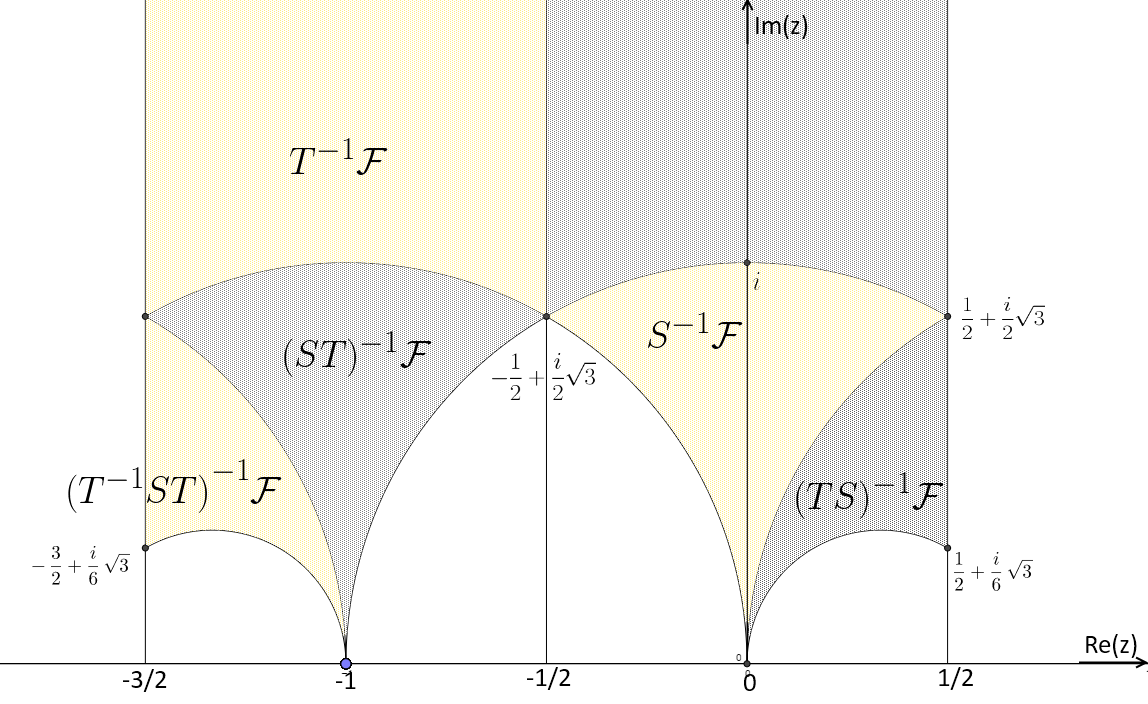
\includegraphics[height=3in]{FundamentalDomainGamma2}
    \else
      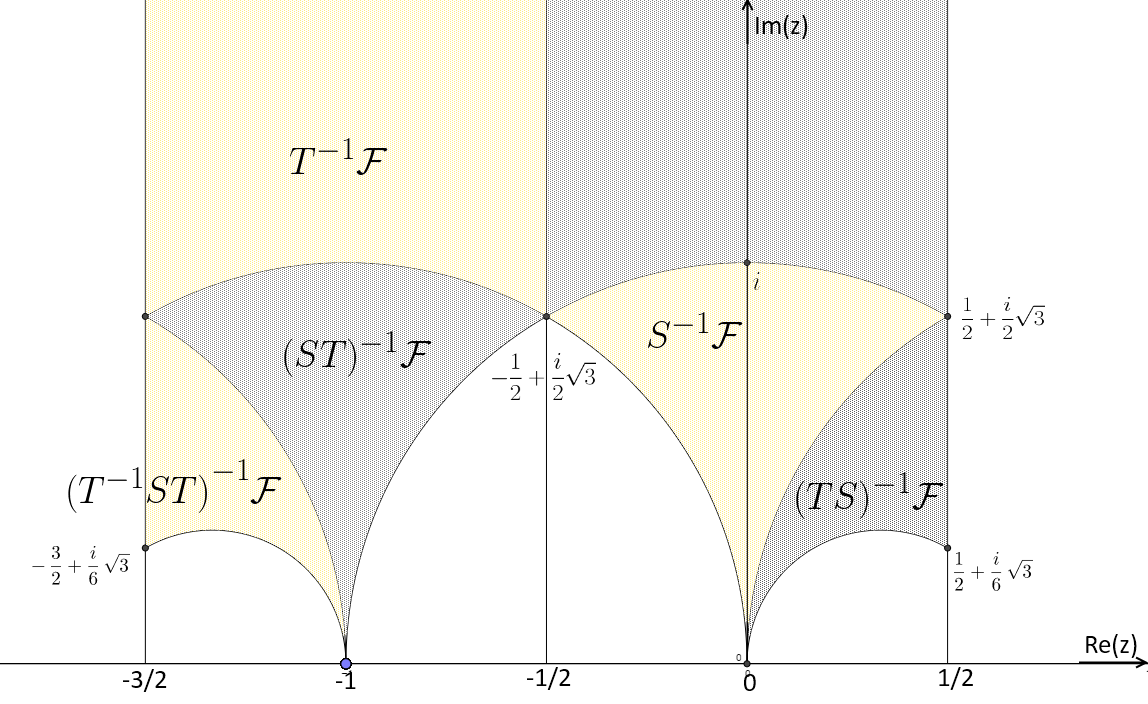
\includegraphics[bb = 92 86 545 742, height=6in]{FundamentalDomainGamma2}
    \fi
    \caption{Example: A Fundamental domain for $\Gamma(2)$}
    \label{fig:funDomainGammaTwo}
  \end{center}
\end{figure}


\end{example}

\begin{remark}
In \citep{verrill} an algorithm is described to construct fundamental domain's for certain congruence subgroups, like $\Gamma(N)$ and $\Gamma_0(N)$, so that the fundamental domain is connected and so that the triangles are "large" when drawn. The Java tool for drawing fundamental domains described in the paper is available at  http://www.math.lsu.edu/~verrill/fundomain/index2.html.
\end{remark}











\numberwithin{equation}{section}
\externaldocument{chapter1}
\externaldocument{chapter2}


\chapter{Non-congruence subgroups of $\sltz$}

\begin{definition}
A non-congruence subgroup $\sltz$ is a finite index subgroup that does not contain $\Gamma(n)$ for any $n$.
\end{definition}

\begin{lemma}\label{lem:compositionFactorsSeries}
Let $G$ be a group with normal series $G = G_0 \geq G_1 \geq \cdots \geq G_r = {1}$, $G_i \trianglelefteq G$. Then the composition factors of $G$ are precisely the union of the composition factors $G / G_1 , G_1 / G_2, \ldots, G_{r-1}/G_r , G_r$.    
\end{lemma}
\begin{proof}
The case $n=0$, $G = G_0 = {1}$ is trivial. We can proceed by induction on $n$. \\
Suppose we have the normal series $G = G_0 \geq G_1 \geq \cdots \geq G_{k+1} = \{1\}$ and that the lemma holds for $n = k$. \\
One can derive the normal series $G_0 \geq G_1 \geq ... \geq G_{k-1} \geq G_{k+1}=\{1\}$ of length $k$ by removing the term $G_k$. So by induction hypothesis, the composition factors of $G_{k+1}$ are the union of the composition factors $G / G_1 , G_1 / G_2, \ldots, G_{k-1}/G_{k+1} , G_{k+1}$. 


We need only show the composition factors for $G_{k-1}$ are the union of the composition factors for $G_k$ and $G_{k-1}/ G_{k}$.\\ 
Consider the refinement 
$$G_{k-1} = A_0 \trianglelefteq \cdots \trianglelefteq A_q = G_k= B_0 \trianglelefteq \cdots \trianglelefteq B_t = G_{k+1 },$$
where the compositions factors $A_{m}/A_{m+1}$ and $B_{j}/B_{j+1}$ are simple. \\
Then since $G_k \triangleleft G_i$ the Third isomorphism theorem gives the normal series $G_{k-1} / G_k = A_0 / G_k\trianglelefteq \cdots \trianglelefteq A_q / G_k = \{e\}$, the factor of a factor part of the theorem gives us that $(A_{m}/H)/(A_{m+1}/H) \cong A_{m}/A_{m+1}$, so the factors are simple and the series is a composition series. The composition factors of $G_{k-1} / H$ are thus equal to (upto isomorphism) the composition factors $A_{m}/A_{m+1}$ of $G_{k-1}/G_{k+1}$  \\
\\
Similarly we can show the composition factors for $G_k/ G_{k+1}$ are the composition factors $B_{j}/B_{j+1}$ of $G_{k-1}/G_{k+1}$.
So the composition factors for $G_{k-1}/G_{k+1}$ are the same as the composition factors for $G_{k-1} / g_k$ and $G_k / G_{k+1}$. \\
We have shown the lemma to be true for $n = k+1$ if it is true for $n = k$, so we can conclude it holds for all $n \in \mathbb{N}$ by induction.
\end{proof}


\begin{remark}

If we have the internal direct product $G = H_1 \times \cdots \times H_n$, then rewriting the element $h_1 \cdots h_n$ as $(h_1, \ldots, h_n )$ we can construct the external direct product which is isomorphic to $G$ under the map $(h_1, \ldots h_n ) \mapsto h_1 \cdots h_n$.
\\
Conversely if $G$ is the external direct product $H_1 \times \cdots \times H_n$ we can define $G_i$ to be the set of all n-tuples of $G$ containing all 1s except (possibly) in $i$th position. Then $G_i \cong H_i$ and $G$ is the internal direct product of $G_1, \ldots , G_n$. 
For these reasons many authors do not distinguish between usage of external and internal direct product.
\end{remark}

\begin{remark}\label{rem:normalDirectProd}
Suppose we have the groups $G_1, G_2, \ldots,  G_n$, and the direct product $G : G_1 \times G_2 \times \cdots \times G_n$. Then we can define the maps 
\begin{eqnarray*}
& \pi_{!G_i} : G \rightarrow G_1 \times \cdots \times G_{i-1} \times  G_{i+1} \times \cdots \times G_n \\
& \pi_{!G_i}(g_1,\ldots g_n) \mapsto (g_1,\ldots, g_{i-1}, g_{i+1},\ldots,g_n)
\end{eqnarray*}
Then we can see that the maps are surjective homomorphisms, and have kernel $\{e\} \times \cdots \times \{e\} \times G_i \times \{e\} \times \cdots \times \{e\} \cong G_i$. \\
This shows each $G_i$ is normal in $G$. 
\\
We can also define the maps $$\pi_{G_i} : G \rightarrow G_i \quad , \quad  \pi_{G_i}((g_1,\ldots, g_i,\ldots,g_n)) \mapsto g_i$$
These are also surjective homomorphisms, and have kernel $G_1 \times \cdots \times G_{i-1} \times \{e\} \times G_{i+1} \times \cdots \times G_1$. We then get the isomorphism 
$$G / (G_1 \times \cdots \times G_{i-1} \times \{e\} \times G_{i+1} \times \cdots \times G_1) \cong G_i$$
\end{remark}


\begin{lemma} \label{lem:compositionFactorDirectProd}
If $G_1, \ldots , G_n$ are non-trivial finite groups then the composition factors of the direct product $G = G_1 \times \cdots \times G_n$ are precisely the union of composition factors of each $G_1, \ldots , G_1$.
\end{lemma}
\begin{proof}
We can use the above remark to get a normal series for $G$, 
$$\{e\} \times \cdots \times \{e\} \vartriangleleft G_1 \times \{e\} \times \cdots \{e\} \vartriangleleft \cdots \vartriangleleft G_1 \times G_2 \times \cdots \times G_m$$
We can apply lemma \ref{lem:compositionFactorsSeries} to conclude that the composition factors for $G$ are the union of composition factors for $(G_1\times \cdots \times G_n)/(\{G_1\} \times \cdots G_{n-1} \cdots \{e\})$, $(G_1 \times \cdots \times G_{n-1} \times \{e\})/(\{G_1\} \times \cdots G_{n-2} \cdots \{e\} \times \{e\})$, \ldots $(G_1 \times \{e\} \cdots \times \{e\})/(\{e\} \times \cdots \times \{e\})$. The above remark also gives that these are isomorphic to $G_n, G_{n-1}, \ldots, G_1 $ respectively. \myqed

\end{proof}  

\begin{lemma}\label{lem:notQuotientDirectProd}
If $S$ is a finite simple group $S$, and $G_1, \ldots , G_n$ are non-trivial finite groups, such that $S$ is not a composition factor of any $G_i$. Then $S$ it is not a composition factor of $G := G_1 \times \cdots \times G_n$. In particular $S$ is not a quotient group of $G_1 \times \cdots G_n$. 
\end{lemma}
\begin{proof}
The Jordan Holder Theorem gives that any two composition series are isomorphic, so if $S$ was a composition factor of $G$ it must be a composition factor of some $G_i$ by lemma \ref{lem:compositionFactorDirectProd}, which it is not by hypotheses so we get a contradiction.\\
If $G$ had a quotient group isomorphic to $S$, then there would be a normal series $\{e\} \times \cdots \{e\} \trianglelefteq N \trianglelefteq G$ with $G/ N \cong S$. This normal series could be extended to a composition series with $S$ as the top composition factor (There are non in-between since $S \cong G/N$ is simple). This is a contradiction to the above. \\
\end{proof}



\begin{theorem}\label{thm:annotquotientsltznz}
For $n \geq 6$ the alternating group $A_n$ is not (isomorphic to) a quotient group of $\sltznz$. for any $N \geq 2$.
\end{theorem}
\begin{proof}
Write $N = p_1^{r_1} \cdots p_m^{r_m}$, so we can apply Proposition \ref{prop:chineseRemainderTheorem} to get 
$$ \sltznz \cong \prod_{i=1}^m \sltznz[p_i^{r_i}].$$
So by lemma \ref{lem:notQuotientDirectProd} it suffices to show that $A_n$ for $n \geq 6$ is not a composition factor of $\sltznz[p^r]$ for any prime power $p^r$.\\
In the proof lemma \ref{lem:orderofslznzpe} we showed that the reduction map $\sltznz[p^r] \rightarrow \sltznz[p]$ is onto. Let $K$ be it's kernel, so we have the normal series, 
$$\{ I_2 \mod p^r \} \trianglelefteq K \trianglelefteq \sltznz[p^r]$$
Then we can apply lemma \ref{lem:compositionFactorsSeries} to say the composition factors of $\sltznz[p^r]$ are the composition factors of $K$ and those of $sltznz / K \cong \sltznz[p]$(By first isomorphism theorem).\\
We begin by considering composition factors of $K$: We have shown in lemma \ref{lem:orderofslznzpe} that the order of $\sltznz[p^r] = p^{3r}(1 - 1/p^2)$, we can use this to compute the order of $K$.
$$\vert K \vert  = \vert \sltznz[p^r] \vert / \vert \sltznz  \vert = \frac{p^{3r}(1 - 1/p^2)}{p^{3}(1 - 1/p^2)} = p^{3(e-1)}$$
This tells us that $K$ is a p-group, and so it's subgroups are p-groups and thus it's composition factors are p-groups so $A_n$ is not a composition factor for $n \geq 6$ since it is not a p-group. \\
Now we can consider the composition factors of $\sltznz[p]$: We use without proof the known fact that $PSL_2(\mathbb{Z}/p\mathbb{Z})$ is simple for $p \geq 5$. The simplicity gives us the composition series $\{I_2\} \vartriangleleft \{\pm I_2 \} \vartriangleleft \sltznz[p]$, recall $ PSL_2(\mathbb{Z}/p\mathbb{Z}) / \{\pm I_2\} \cong \sltznz[p]$. So we get the composition factors $\znz[2]$ and $PSL_2(\mathbb{Z}/p\mathbb{Z})$ for $p \geq 5$. In the case $p =2$, we have $\sltznz[2] = GL_2(\mathbb{Z}/2\mathbb{Z}) \cong S_3$, and in the case $p = 3$ we have $\sltznz[3] /\{\pm I_2\} \cong A_4$, the composition factors of these groups are cyclic ( of order 2 or 3).
\\
We have shown that the only case where $A_n$ could possibly be a composition factor of $\sltznz[p^r]$ is if $A_n \cong \psltznz[p]$ and $p\geq5$. We can show this never occurs by comparing the sizes of the two groups. \\
The group $\psltznz[p]$ has order $\vert \sltznz[p] \vert /2 = (p^2 -1)p/2$,  and the group $A_n$ has order $n!/2$, we seek
$$(p-1)p(p+1) = n!$$
If $n < p$ then $n!$ is not divisible by $p$ and we have a contradiction. If $n = p$ when we obtain the equation $p+1 = (p-2)!$, we can check the only solution is $p = n =5$. If $n = p+1$ then dividing both sides by $(p-1)p(p+1)$ we get $1 = (p-2)!$ so $p = 3$ or $p =2$, but we need $p \geq 5$. The final case where $n \geq p +2$ then $n! > (p-1)p(p+1)$. \\
The only solution we found was $n = p =5$( and indeed it can be shown $\psltznz[5] \cong A_5$), for $n \geq 6$ the group $A_n$ is not a quotient group of $\sltznz$ for any $N \geq 2$. 

\end{proof}


\begin{theorem}\label{thm:anquotientsltz}
For $n \geq 9$, $A_n$ is a quotient of $\sltz$.
\end{theorem}

\begin{proof}
We will actually get $A_n \cong \psltz / K$, but since $\psltz = \sltz / \{\pm I_2\}$ we can use the correspondence theorem to say $K = N / \{\pm I_2\}$ for some $N \lhd \sltz$. Which by the factor of a factor theorem means we get $ \sltz / N \cong A_n$, and so $A_n$ is a quotient of $\sltz$.\\
We use two principal facts to prove this result: $A_n$ (for $n\geq 9$) is generated by two elements of order 2 and 3, and $\psltz$ is also freely generated by two elements of order 2 and 3. In 1901, G. A Miller first constructed generating elements of order 2 and 3 for $A_n$ \citep{miller}. \\
We showed in Theorem \ref{cor:genFiniteOrderSST} that $S, ST$ generate $\sltz$ and so every element in $\psltz$ can be written as a product of $x = \bar{S} = S/\pmi\, ,\, y= \bar{ST} = ST \pmi$ and these have order 2 and 3. We can then write any product of $x,y$ in "reduced" form,
$$ y^{i_0}xy^{i_1}x \cdots y^{i_{n-1}}xy^{i_n},$$
where the exponents $i_j$ are taken $\znz[3]$ and they are nonzero modulo 3 except possibly $i_0$ and $i_n$. Now since we have shown $\psltz$ to be freely generated it means each such representation is unique. \\
Following from this, suppose we have another group $G = \langle a ,b \rangle$ where $a,b$ have order 2 and 3. A map $f \, : \, \{x, y\} \rightarrow \{a , b\}$ where $f(x) = a, \, f(y) = b$ and $f' \, : \, \psltz \rightarrow G$ extends uniquely to a homorphism $f' \, : \psltz \rightarrow G$. I.e there is a unique homorphism $f'$ such that $f'(x) =a$ and $f'(y) = b$\\
The uniqueness is readily proven. Let $ s \in \psltz$, then we can write s as a word in in reduced form $x,y$, $s = y^{i_0}xy^{i_1}x \cdots y^{i_{n-1}}xy^{i_n}$,  
\begin{eqnarray*}
f'(y^{i_0}xy^{i_1}x \cdots y^{i_n-1}xy^{i_n}) &\stackrel{f'\text{ hom.}}{=}& f'(y)^{i_0}f'(x)f'(y)^{i_1}f'(x) \cdots f'(y)^{i_{n-1}}f'(x)f'(y)^{i_n} \\
&=& f(y)^{i_0}f(x)f(y)^{i_1}f(x) \cdots f(y)^{i_{n-1}}f(x)f(y)^{i_n}
\end{eqnarray*} 
Since $\psltz$ is freely generated by $x, y$ the representation for $s$ is unique and so there is no other possible value for $f'(s)$. \\
The homomorphism $f'$ is also surjective, given any element $c \in G$ we can write it in "reduced" form as a word in $a,b$, $c = a^{j_0}ba^{j_1}b\cdots a^{j_{k-1}}ba^{j_k}$. And then $f'(y^{j_0}xy^{j_1}x \cdots y^{j_{k-1}}xy^{i_k}) = c$.\\
The First Isomorphism theorem gives us that $\psltz / ker(f') \cong A_n$.
\end{proof}

\begin{example}
The group $A_9$ turns out to be generated by
$$(14)(29)(37)(56) \text{ and } (123)(456)(789),$$
so one surjective homorphism from $\sltz$ to $A_9$ is the composite map $\sltz \rightarrow \psltz \rightarrow A_9$ where the first map is reduction $\mod \pmi$ and the second is determined by $\bar{S} \mapsto (14)(29)(37)(56)$ and $\bar{ST} \mapsto (123)(456)(789)$. \\
Note this is not going to be the only homomorphism, for example $A_9$ will also be generated by $((14)(29)(37)(56))^{-1}$ and $(23)(456)(789)$ so we can define another composite map with $\bar{S} \mapsto ((14)(29)(37)(56))^{-1}$ instead. \\ 
\end{example}

\begin{corollary} \label{cor:annoncongruence}
Let $\phi \, : \, \sltz \rightarrow A_n$ be a surjective homomorphism. Then the kernel of $\phi$ is a non-congruence subgroup. 
\end{corollary}

\begin{proof}
Let $\phi \, : \, \sltz \rightarrow A_n$ be a surjective homomorphism, with kernel $K$. So we have $\sltz / K \cong A_n$. The kernel, $K$ will have finite index of order $\vert A_n \vert = n!/2$. Suppose we had $\Gamma(N) \subset K$. Recall kernels of homorphisms are normal subgroups so we get the normal series, $\{I_2\} \subset \Gamma(N) \subset K \subset \sltz$. We can apply the Factor of a Factor theorem to say $  (\sltz / \Gamma(N)) / (K / \Gamma(N)) \cong \sltz / K \cong A_n$. Then since $\sltz / \Gamma(N) \cong \sltznz$, we arrive at 
$$\sltznz / (K/ \Gamma(N) \cong A_n.$$
This implies $A_n$ is a quotient group of $\sltznz$ but this raises a contradiction by Theorem \ref{thm:annotquotientsltznz}. So the kernel $K$ is a finite index non-congruence subgroup of $\sltz$.
\end{proof}

\begin{remark}
We can construct matrices in the $\ker \phi$ non-congruence subgroup and also check if matrices are in it. For $n \geq 9$ pick two elements $x$ and $y$ in $A_n$ or respective orders 2 and 3 such that $A_n = \langle x , y\rangle$. To construct a matrix in the subgroup, take an element $a \in A_n$ such that it can be written as a "reduced" word in $x,y$ in two different ways, 
$$ a = y^{i_0}xy^{i_1}x \cdots y^{i_{n-1}}xy^{i_n} =  y^{j_0}xy^{j_1}x \cdots y^{j_{k-1}}xy^{j_k}$$
(This is possible since $A_n$ is not freely generated). The product of the first word and the inverse of the second will be the identity. 
$$I = y^{i_0}xy^{i_1}x \cdots y^{i_{n-1}}xy^{i_n}( y^{-j_k}xy^{-j_{k-1}} \cdots xy^{-j_1}xy^{-j_0} )$$
Now replace each $x,y$ by $S, ST$ respectively and you get matrix, $A$, in the kernel of the map $\phi$. I.e 
$$A = (ST)^{i_0}S(ST)^{i_1}S \cdots (ST)^{i_{n-1}}S(ST)^{i_n} \cdot (ST)^{-j_k}S(ST)^{-j_{k-1}} \cdots S(ST)^{-j_1}S(ST)^{-j_0}$$
The matrix will not be the identity matrix since $\psltz$ is freely generated.\\
In the reverse direction, take a matrix $A \in \sltz$ and write it (up to an overall sign) as a product of $S$ and $ST$. Turn that word in $S$ and $ST$ into a word in $x$ and $y$. The matrices whose corresponding word in $x$ and $y$ is trivial form a non-congruence subgroup of $\sltz$. \\

More general algorithms are known that could find the generators of $\ker \phi$ but are beyond the scope of this project. It would be an interesting exercise to try this in the future, perhaps with use of computer algebra systems like GAP. 
\end{remark}

\begin{remark}
The procedures used in the proofs of Theorems \ref{thm:annotquotientsltznz} \& \ref{thm:anquotientsltz} in order to construct a non congruence subgroup can be generalized in order to find other non-congruence subgroups.\\
The steps are the same, we must find a finite simple non-abelian group that is not a quotient of $\sltznz$ but is a quotient of $\sltz$, then by the same steps as in \ref{cor:annoncongruence}, this group is isomorphic to $\sltz /N $ where $N$ is a non-congruence subgroup.\\
In order to show a finite simple non-abelian group is not a quotient of $\sltznz$ we have shown it is sufficient to show it is not isomorphic to $\psltznz[p]$ for some prime $p \geq 5$ where $p \vert N$.\\
In order to show it is a quotient of $\sltz$ we have shown it to be sufficient that it is generated by a pair of elements with order 2 and 3. \\
\end{remark}

The above sufficient conditions in order to find a non-congruence subgroup are actually satisfied by most non-abelian finite simple groups. The classification of finite simple groups allows us to find many groups of this form.

\begin{remark}
The classification of finite simple groups gave a result that all non-abelian finite simple groups have rank 2. I.e they can all be generated by two elements. We desire that the groups are so called (2,3)-generated, I.e that they can be generated by an element of order 2 and 3. The results about (2,3)-generated groups are taken from the book Groups of Lie Type and Their Geometries\citep{kantorGenerated}.
We have already stated that the alternating groups $A_n$ for $n \geq 9$ are all (2,3)-generated.\\
In 1989 it was shown by Woldar that the non-abelian finite simple groups belonging to the family called Sporadic groups are all (2,3) generated with the exception of the groups denoted $M_{11},\, M_{22},\, M_{23},\, McL$. \\
In 1990 Malle showed that the Chevalley groups $G_2(q)$ and the twisted groups $^2G_2(q), ^3D_4(q)$ and $^2F_4(q)$ are (2,3)-generated.\\

Due to the classification of finite simple groups it is known that none of these are isomorphic to $\psltznz[p]$ for any prime $p \geq 5$ so none of them are quotients of $\sltznz$ where $ P \vert N$. \\
So for each of the groups $G$ above satisfying both conditions, we can construct a surjective homomorphism $\phi \, : \sltz \rightarrow G$ and the kernel of $\phi$ will be a finite-index non-congruence subgroup.

\end{remark}

The proof of the following Theorem was derived from Alperin \citep{alperinpsl}.
\begin{theorem}
The group $\psltz$ is freely generated by two elements of order two and three. I.e $\psltz \cong C_2 * C_3$.
\end{theorem}
\begin{proof}
We consider the action of $\psltz$ by linear fractional transformations on the extended complex plane, like discussed in Chapter 2. In particular it's action on the irrational numbers. Explicitly if $z$ is an irrational number and $\abcd \in \sltz$, we have the action 
$$ \abcd (z) = \frac{az + b}{cz +d}.$$
We use irrational numbers since unlike rational numbers the denominator will never be zero, since if it was zero then would have $cz +d = 0 \implies z = -d/c \mathbb{Q}$ which is a contradiction.\\
The action also preserves irrationality: Suppose for some irrational $z$ and some $\abcd \in \sltz$ we had $\frac{az + b}{cz +d} = m/n$ with $m/n \in \mathbb{Q}$ and $\gcd(m,n) =1$. Then we could rearrange to get 
$z(ay - cx) =  dx - by$. Now since $(x,y) = 1$, we get $ay-cx = 0 \iff a=x, c=y$. If then must also have $d=y,b=x$, so $ad -bc = xy - xy = 0$ which is a contradiction, so $ay - cx \neq 0$. This means we could write $z = \frac{dx -by}{ay -cx} \in \mathbb{Q}$ which is a contradiction.\\

We have shown in Corollary \ref{cor:genFiniteOrderSST} that $S, ST$ are matrices of order 2 and 3 (in $\psltz$) that generate $\psltz$, so we also have that $S = \left(\begin{array}{ c c } 0 & -1 \\ 1 & 0 \end{array} \right) \,,\, TS = \left(\begin{array}{ c c } 1 & -1 \\ 1 & 0 \end{array} \right)$ are matrices of order 2 and 3 that generate $\psltz$. Their action on the irrational numbers is, 
\begin{eqnarray*}
S(z) &=& \left(\begin{array}{ c c } 0 & -1 \\ 1 & 0 \end{array} \right)(z) = \frac{-1}{z} \\
TS(z) &=& \left(\begin{array}{ c c } 1 & -1 \\ 1 & 0 \end{array} \right)(z) = \frac{z-1}{z}\\
{(TS)}^{-1}(z) &=& \left(\begin{array}{ c c } 0 & 1 \\ -1 & 1 \end{array} \right)(z) = \frac{1}{1-z}
\end{eqnarray*}
Alternating word are of the form $S^{k_1}(TS)^{j_1}S^{k_2}(TS)^{j_1}\cdots S^{k_n}(TS)^{j_n}$, where $j_i, k_i \neq 0$.
In order to prove $\psltz$ is a free group we show that if we take a word in $\{S,TS,{(TS)}^{-1}\}$ that is alternating from $S$ to $(TS)^{\pm 1}$ then is not the identity. This is called the alternating word characterization and is equivalent to the definition a free group. (If we could find an alternating word that is the identity then the group would not be free. Conversely if the group was not free then we could find an element that can be written as two distinct alternating words, so the inverse of the first times the second is an alternating word representation for the identity).
\\ 
We make use of the following properties of the action of $S$ and ${(TS)}^{\pm 1}$. Let us denote $\mathcal{P}$ as the set of positive irrationals and $\mathcal{N}$ as the set of negative irrationals. We an observe that, 
$$ S(z) = -1/z \implies S(\mathcal{P}) \subset \mathcal{N}$$
and,
$$(TS)(z) = 1 - \frac{1}{z} \text{ and } {(TS)}^{-1}(z) = \frac{1}{1-z} \implies {(TS)}^{\pm 1}(\mathcal{N}) \subset \mathcal{P}.$$
suppose we have a word $w$ that is alternating from $\{S\}$ to $\{{(TS)}^{\pm 1}\}$. The core idea is that we can use the alternating effect to determine whether $w(\mathcal{P})$ or $w(\mathcal{N})$ are subsets of $\mathcal{P}$ or $\mathcal{N}$. For notation we use, $\alpha = S, \beta = TS$\\
\\
If the word has odd length, then it either begins and ends with $\alpha$ or begins and ends with ${\beta}^{-1}$. \\
In the first case we can consider $w(\mathcal{P}) = \alpha ({\beta}^{i_0}\alpha)\cdots ({\beta}^{i_k} \alpha) ( \mathcal{P})$. For each pair we have $({\beta}^{\pm 1} \alpha) (\mathcal{P}) \subset ({\beta}^{\pm 1})(\mathcal{N}) \subset \mathcal{P}$. So we are left with $\alpha(\mathcal{P}) \subset \mathcal{N}$, i.e $w(\mathcal{P}) \subset \mathcal{N}$.\\
In the second case we can consider $w(\mathcal{N}) = {\beta}^{i_0}(\alpha{\beta}^{i_1}) \cdots (\alpha{\beta}^{i_n})(\mathcal{N})$. For each pair we have $({\beta}^{\pm 1}\alpha)(\mathcal{N}) \subset \mathcal{N}$. So we are left with ${\beta}^{i_0}(\mathcal{N}) \subset \mathcal{P}$, i.e $w(\mathcal{N}) \subset \mathcal{P}$.\\
\\
If the word has even length, then it either begins with $\alpha$ and ends with ${\beta}^{\pm 1}$ or vice versa. If it begins with $\alpha$ we can take the conjugate by $\alpha$ so we need only consider the one case, we will reconcile this afterwords. \\
In the first case, $w = \beta \cdots \alpha $. We can use the same "pairing" reasoning as above to get $w(\mathcal{P}) \subset \beta (\mathcal{N})$ which by looking at the function $\beta$ we can see is the set of positive irrationals greater than one.\\
In the other case, $w = {\beta}^{-1} \cdots \alpha$, and similarly we get $W(\mathcal{P}) \subset {\beta}^{-1}(\mathcal{N})$, this is the set of positive irrationals less than one.\\
\\
We have shown that in all cases there will exist an irrational $z$ such that $w(z) \neq z$. (Example: if $w$ is an even length word beginning with $\beta$ and we take $z =\sqrt{2}$, we've shown $w(z) < 1$ but $\sqrt{2} >1$ so $w(z) \neq z$). \\
In conclusion we have shown for any word $w$ that is alternating from $\{S\}$ to $\{{(TS)}^{\pm 1}\}$ it is not the identity. (In the case of taking the conjugate, if ${\alpha}^{-1}w\alpha \neq I_2 \implies w \neq I_2$). So by the alternating word characterization we get $\psltz \cong C_2 * C_3$.
\end{proof}

\subsection{More examples of non congruence subgroups}
The following section is from Chapter 3 in the book  \textit{The congruence subgroup problem: an elementary approach aimed at applications} \citep{suryCongruence}.
\begin{example} \label{ex:noncongruenceEA}
It's possible to give a more explicit construction of a non-congruence subgroup.
\\
It is shown in \citep{suryCongruence} that the group $G$ generated by $A:=T^2 =\left(\begin{array}{ c c } 1 & 2 \\ 0 & 1 \end{array} \right) $ and $B:= U^2 = \left(\begin{array}{ c c } 1 & 0 \\ 2 & 1 \end{array} \right)$ is free and has index 2 in $\Gamma(2)$.\\
For any word $w$ in $ A, B$ we may define the $T^2$-exponent $E_A(w)\,: \, G \rightarrow \mathbb{Z}$ of $w$ to be the sum of the exponents of $A$ occurring in $w$. \\
We can show this defines a homomorphism from $G$ to $\mathbb{Z}$: For any $w \in G$ there is a unique representation, excluding trivial variations in $A,B$, since $G$ is a free group. The trivial variations, eg $ w = ABA = A(AA^{-1})BA$ cancel out and do not affect $E_A(w)$, this makes the map well defined. \\
Let $w_1, w_2 \in G$, then the product $W_1 w_2$ can simply be thought of as a concatenation of the two words and as a result we get $E_A(w_1 w_2) = E_A(w_1) + E_A(w_2)$. \\
\\
For any integer $l \geq 1$, let us define
$$\Gamma_{l}^A = \{ g \in G \, : \, E_A(g) \equiv 0 \mod l\} = Ker(G \rightarrow \mathbb{Z} \rightarrow \znz[l])$$
\begin{figure}
\centering

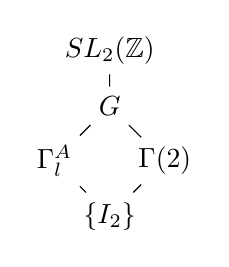
\begin{tikzpicture}[scale=.7]
  \node (sltz) at (0,2) {$\sltz$};
  \node (g) at (0,1) {$G$};
  \node (gl) at (-1,0) {$\Gamma_{l}^A$};
  \node (g2) at (1,0) {$\Gamma(2)$};
  \node (i) at (0,-1) {$\{I_2\}$};
  \draw  (sltz) -- (g) --(gl) -- (i) --(g2) -- (g);  % (a) -- (one) -- (b) -- (zero) -- (c) -- (one) -- (d) -- (zero);
\end{tikzpicture}
\caption{Hasse diagram} \label{fig:hasseDiagram}
\end{figure}

We claim that $\Gamma_{l}^A$ is a non-congruence subgroup if $l$ is not a power of 2.\\ 
Now since $\Gamma(lt) \subset \Gamma(t)$ it suffices to show $ \Gamma(tl) \not\subset \Gamma_l$ for any $t$. We can write $l = 2^q*k$ where $k >1$ odd. From this we can rewrite $ln = 2^q k t = 2^mkn$ with $n$ odd. For the sake of contradiction let us suppose $\Gamma(2^t kn) \subset \Gamma_{l}^A$ for some $m \geq 0$ and odd $n$. \\
The integers $2^m5kn$ and $5kn -4$ are comprime, $2$ is not a common divisor since $5kn -4$ is odd, and also if an odd prime $p \vert 2^m5kn \implies p\vert 5kn$ so it will not divide $5kn -4$. There exists an integer $s$ such that $s(5kn -4) \equiv 1 \mod 2^m5kn$, i.e $s(5kn -4) = 1 + (2^m5kn)h$ for some $h \in \mathbb{Z}$. If we consider this equation modulo 5, we get $s \equiv 1 \mod 5$. Let us write $s = 5r +1$. \\
The matrix $P = B^rABA^{kn-1} =  \left(\begin{array}{ c c } 5 & 2(5kn -4) \\ 2s & \delta \end{array} \right) \in G$ for some $\delta$. Note that the condition on the determinant $\det(P) = 1$ gives $\delta \equiv 1 \mod 2^mkn$, ($\star$). \\
We can also consider the matrix $Q = A^{5kn -4}B^s =  \left(\begin{array}{ c c } \alpha & 2(5kn -4) \\ 2s & 1 \end{array} \right) \in G$ for some $\alpha$. Again the condition on the determinant is $5\delta - 4s(5kn -4) =1$, now consider this modulo $2^m5kn$ and use $(\star)$, to get $5\delta \equiv 5 \mod 2^m5kn$. This implies that $\alpha \equiv 5 \mod 2^m5kn \implies \alpha \equiv 5 \mod 2^mkn$. 

Therefore we can see by considering each entry that $P \equiv Q \mod 2^mkn$. In other words, $PQ^{-1} \in \Gamma(2^mkn)$. But, $E_A(PQ^{-1}) = 1 + (kn-1) + 4 - 5kn = -4kn + 4 \equiv 4 \not \equiv 0 \mod k$.Hence $E_A(PQ^{-1}) \not\equiv 0 \mod l$. This contradicts our assumption that $\Gamma(2^mkn) \subset \Gamma_{l}^A$. Hence, $\Gamma_{l}^A$ cannot be a congruence subgroup.\\
\\
We can determine the index of $\Gamma_{l}^A$. From figure \ref{fig:hasseDiagram} we have, 
$$[\sltz \, : \,\Gamma_{l}^A]= [\sltz \, : \, G][G \, : \, \Gamma_{l}^A] =[\sltz \, : \, G]\cdot \vert \znz[l] \vert = [\sltz \, : \, G]\cdot l$$
Also,
$$ [\sltz \, : \, G] = \frac{[\sltz \, : \, \Gamma(2)]}{[G \, : \, \Gamma(2)]} = \frac{6}{2} =3.$$
So we have $[\sltz \, : \, \Gamma_{l}^A] = 3l$.
\end{example}

\subsection{Local versus index - a criterion}

\begin{theorem} {'Wohlfahrt's criterion'} \label{thm:criterion}\\
Let $G \leq \sltz$ be a subgroup of finite index. Suppose $n$ is a positive integer such that $G \supset \gamma \left(\begin{array}{ c c } 1 & n \\ 0 & 1 \end{array} \right) \gamma^{-1}$ for every $\gamma \in 
\sltz$. Then, $G$ is a congruence subgroup if, and only if, $G \geq \Gamma(n)$. (The notation $G \geq H$ means $H$ is a subgroup of $G$.)
\end{theorem}
\begin{proof}
If $G \geq \Gamma(n)$ then by definition it is a congruence subgroup. \\
For the reverse implication let us assume that $G$ is a congruence subgroup, $G \geq \Gamma(m)$ for some $m$, and that there is a $n$ such that $G \supset \gamma \left(\begin{array}{ c c } 1 & n \\ 0 & 1 \end{array} \right) \gamma^{-1}$ for every $\gamma \in sltz$. (Note in particular $\left(\begin{array}{ c c } 1 & n \\ 0 & 1 \end{array} \right) \in G$).
We wish to show that $G \geq \Gamma(n)$. \\
Let $g = \abcd \in \Gamma(n)$. From the determinant we get $\det(g) = ad -bc = 1 \implies (a,c) =1$ and also since $g \in \Gamma(n)$ we have $n \vert c$ so $(a,nc) =1$. From Lemma \ref{lem:elementaryCoprime} we can find $x \in \mathbb{Z}$ such that $(a + ncx,m) = 1$. Therefore, there exists $y$ such that $y(a + ncx) \equiv 1 \mod m$ $(\star)$. \\
Now let $g_1$ be the product, 
$$g_1 = \left(\begin{array}{ c c } 1 & nx \\ 0 & 1 \end{array} \right)g =  \left(\begin{array}{ c c } a + ncx & b+ndx \\ c & d \end{array} \right) \in \Gamma(n)$$
Moreover from the assumption about $G$, we have for any integer $z$, if we let,
$$g_2 := \left(\begin{array}{ c c } 1 +nz & -n \\ nz^2 & 1-nz \end{array} \right) = \left(\begin{array}{ c c } 1 & 0 \\ z & 1 \end{array} \right) \left(\begin{array}{ c c } 1 & -n \\ 0 & 1 \end{array} \right)\left(\begin{array}{ c c } 1 & 0 \\ -z & 1 \end{array} \right) $$
Then the matrix $g_2$ is in $G$ since it is the inverse of a matrix of the form $\gamma  \left(\begin{array}{ c c } 1 & n \\ 0 & 1 \end{array} \right) \gamma^{-1}$n and $g_2 \in \Gamma(n)$.\\
We have $g_2 g_1 = \left(\begin{array}{ c c } (1+nz)(a+ncx) -nc & \star \\  \star &  \star \end{array} \right)$.\\
If we choose $z = y(c(1-x) + \frac{1-a}{n})$, we get 
\begin{eqnarray*}
(1+nz)(a + ncx) -nc &=& (1 + ny(c(1-x) + \frac{1-a}{n})(a + ncx) - nc \\
&=& a+ncx + ny(a+ncx)(c(1-x) + \frac{1-a}{n} \\
\text{ use } (\star) &=& a + ncx + n(1 +mt)(c(1-x) + \frac{1-a}{n} \text{ for some } t \in \mathbb{Z} \\
&=& a + ncx + nc - ncx + 1 -a + nmt(c(1-x)) + mt(1-a) \\
& = & 1 + (1-a)mt + nmt(c(1-x)) \\
(a \equiv 1 \mod n) & \equiv & 1 \mod mn  
\end{eqnarray*}
Let
$$h = \left(\begin{array}{ c c } 1 +nz & -n \\ nz^2 & 1-nz \end{array} \right) = \left(\begin{array}{ c c } 1 & 0 \\ z & 1 \end{array} \right) \left(\begin{array}{ c c } 1 & -n \\ 0 & 1 \end{array} \right)\left(\begin{array}{ c c } 1 & 0 \\ -z & 1 \end{array} \right)\left(\begin{array}{ c c } 1 & nx \\ 0 & 1 \end{array} \right),\quad  z = y(c(1-x) + \frac{1-a}{n}).$$
Then by inspection we see $h \in G \cap \Gamma(N)$. Now consider $hg \in \Gamma(n)$.\\
The matrix $hg$ can be written in the form $\left(\begin{array}{ c c } \star & nu \\ nv & \star \end{array} \right)$ since $hg \in \Gamma(n)$.\\
From the work above we also have $hg \equiv \left(\begin{array}{ c c } 1 & \star \\ \star & \star \end{array} \right) \mod mn$. So we combine these to get $ hg  \equiv \gamma = \left(\begin{array}{ c c } 1 & nu \\ nv & \star \end{array} \right) \mod mn$.\\
The condition on the determinant gives $\gamma \equiv  \left(\begin{array}{ c c } 1 & nu \\ nv & 1 + n^2uv \end{array} \right) \mod mn$.
We may decompose this as 
\begin{align*}
\gamma &\equiv  \left(\begin{array}{ c c } 1 & 0 \\ nv & 1 \end{array} \right) \left(\begin{array}{ c c } 1 & nu \\ 0 & 1 \end{array} \right) \\
&\equiv \left(\begin{array}{ c c } 0 & 1 \\ v & 0 \end{array} \right) \left(\begin{array}{ c c } 1 & n \\ 0 & 1 \end{array} \right) {\left(\begin{array}{ c c } 0 & 1 \\ v & 0 \end{array} \right)}^{-1} \left(\begin{array}{ c c } u & 0 \\ 0 & 1 \end{array} \right)^{-1}\left(\begin{array}{ c c } 1 & n \\ 0 & 1 \end{array} \right) \left(\begin{array}{ c c } u & 0 \\ 0 & 1 \end{array} \right)
\end{align*}
So if consider $\gamma' =  \left(\begin{array}{ c c } 1 & nu \\ nv & 1 + n^2uv \end{array} \right) \equiv \gamma$ be an element in $\sltz$, then $\gamma' \in G$.\\
\\
We use, $\gamma^{-1}hg \equiv I_2 \mod mn$, to say $\gamma'^{-1}hg \in \Gamma(mn) \leq \Gamma(m) \leq G$. Finally since $\gamma',g \in G$ we can conclude $g \in G$ and so $\Gamma(n) \leq G$.
\end{proof}

\begin{example}
We can use the above criterion to obtain another example of a non-congruence subgroup. \\
Let us recall the homomorphism $E_A \, : \, w(A,B) \rightarrow \mathbb{Z}$ from Example \ref{ex:noncongruenceEA}, and define $E_B \, : \, w(A,B) \rightarrow \mathbb{Z}$ similarly, as the sum of the exponents of $B$ occurring in a word $w$. From these we can define a new homorphism, $E_{A,B} \, : \, w(A,B) \rightarrow \mathbb{Z} \times \mathbb{Z}$, where $E_{A,B}(w) = (E_A(w), E_B(w))$.\\ 
For a positive integer $l$ let us define 
\begin{eqnarray*}
\Gamma_{l}^{A,B} &=& \{g \in w(A,B) \, :\, E_A(g) \equiv E_B(g) \equiv 0 \mod l\} \\
\ker(w(A,B) & \rightarrow & \mathbb{Z} \times \mathbb{Z} \rightarrow \znz[l] \times \znz[l]
\end{eqnarray*} This group is a subgroup of the non-congruence subgroup, $\Gamma_{l}^A$ from example \ref{ex:noncongruenceEA}.\\

We claim: If $l$ is not a power of 2. then $\Gamma_l$ is not a congruence subgroup. \\
If it were a congruence subgroup, then $\Gamma_p \geq \Gamma_l$ would also be a congruence subgroup for any odd prime divisor $p$ of $l$.

Consider the matrix, $A^{2p} = \left(\begin{array}{ c c } 1 & 2p \\ 0 & 1 \end{array} \right) \in \Gamma_p$, then for any $\gamma \in \sltz$ we have $E_A(\gamma A^p \gamma^{-1}) = E_A(\gamma) + E_A(A^p)+ E_A(\gamma^{-1}) = E_A(\gamma) + E_A(A^p) - E_A(\gamma) = E_A(A^p) = p \equiv 0 \mod p$, and similarly $E_B(\gamma A^p \gamma^{-1}) = E_B(\gamma A^p) = 0 \equiv 0 \mod p$. So $\gamma A^p \gamma^{-1} \in \Gamma_p$ and the criterion in Theorem \ref{thm:criterion}, is satisfied for $n = 2p$, thus $ \Gamma_p \geq \Gamma(2p)$.
\\
Thus the index $[\sltz \, : \, \Gamma_p]$ divides $[\sltz \,: \, \Gamma(2p)]$. We will see that this gives a contradiction.
\\

We obtained an expression for index's of congruence subgroups in Corollary \ref{cor:indexListChain},
 $$[\sltz \,: \, \Gamma(2p)] = (2p)^3\prod_{p \mid 2p}(1 - 1/p^2) = 8p^3( 1 - 1/4)(1 - 1/p^2) = 6p(p^2 -1)$$
\\
From the presentation of $\Gamma_p$ as a kernel, we get that the index $[w(A,B) \, : \, \Gamma_p] = \vert \znz[p] \times \znz[p] \vert = p^2$. We computed in Example \ref{ex:noncongruenceEA}, that $[\sltz \, : \, w(A,B)] = 3$ so we can combine these two to get $[\sltz \, : \, \Gamma_p] = 3p^2$. 
\\
Suppose then that $[\sltz \, : \, \Gamma_p] \vert [\sltz \,: \, \Gamma(2p)]$, then $$3p^2 \vert 6p(p^2 -1) \implies p \vert 2(p^2 -1) \stackrel{\text{p odd}}{\implies} p \vert (p^2 -1) $$

This is a contradiction so $\Gamma_l$ cannot be a congruence subgroup if it contains an odd prime factor.
\end{example}

\section{Conclusion}
For another construction of non-congruence subgroups see \citep{hsu1996identifying}, in this a method, based on permutation representations of $\psltz$, of identifying congruence subgroups is detailed.\\
The question of determining whether or not finite-index subgroup of $\sltz$ that are not congruence subgroups exist, is more generally known as the Congruence Subgroup Problem. We have shown they do exist for $\sltz$ but it is easy to pose the problem similarly for $SL_n(\mathbb{Z})$. It was actually shown in \citep{bass1964} that for $n > 2$ every finite index subgroup of $SL_n(\mathbb{Z})$ are congruence subgroups. \\
Even further it is possible to define the notion of congruence for more general number fields $K$, a more general result about $SL_n(\mathcal{O}_K$ is proven in \citep{bassSolution}.\\
\\
Python code written for this project is available at https://github.com/MarcoForte/UndergradThesis
The code includes, the generating of the images, and implementations of algorithms like those described geometric and algebraic proof that $\langle S, T \rangle = \sltz$.
%\def\baselinestretch{1}
\chapter{My Conclusions ...}
\ifpdf
    \graphicspath{{Conclusions/ConclusionsFigs/PNG/}{Conclusions/ConclusionsFigs/PDF/}{Conclusions/ConclusionsFigs/}}
\else
    \graphicspath{{Conclusions/ConclusionsFigs/EPS/}{Conclusions/ConclusionsFigs/}}
\fi

\def\baselinestretch{1.66}

Here I put my conclusions ...

%%% ----------------------------------------------------------------------

% ------------------------------------------------------------------------

%%% Local Variables: 
%%% mode: latex
%%% TeX-master: "../thesis"
%%% End: 


\backmatter % book mode only
%\appendix
%\chapter{Appdx A}

and here I put a bit of postamble ...

% ------------------------------------------------------------------------

%%% Local Variables: 
%%% mode: latex
%%% TeX-master: "../thesis"
%%% End: 

%\chapter{Appdx B}

and here I put some more postamble ...

% ------------------------------------------------------------------------

%%% Local Variables: 
%%% mode: latex
%%% TeX-master: "../thesis"
%%% End: 


\bibliographystyle{plainnat}
%\bibliographystyle{Classes/CUEDbiblio}
%\bibliographystyle{Classes/jmb}
%\bibliographystyle{Classes/jmb} % bibliography style
\renewcommand{\bibname}{References} % changes default name Bibliography to References
\bibliography{References/references} % References file

\end{document}
